\chapter{Transition vers l'écoulement des fluides à seuil}

\label{chapter:yielding}

\subparagraph{}Dans le \autoref{chapter:introduction}, nous avons vu que la transition vers l'écoulement peut être comprise comme une transition de phase absorbante. Le paramètre de contrôle est alors la contrainte imposée au système $\Sigma$ et le paramètre d'ordre le taux de déformation $\dot{\gamma}$. Ce dernier est nul dans la phase absorbante pour $\Sigma < \Sigma_c$ et non-nul dans la phase active pour $\Sigma > \Sigma_c$. Proche de la transition, l'évolution de $\dot{\gamma}$, de sa variance $\langle\Delta\dot{\gamma}^2\rangle$ et de la longueur de corrélation $\xi$ sont dictées par les exposants critiques $\beta, \gamma^\prime$ et $\nu_\perp$ selon :

\begin{equation}
	\dot{\gamma} \sim \delta\Sigma^\beta,\quad \langle\Delta\dot{\gamma}^2\rangle \sim \delta\Sigma^{-\gamma^\prime}, \quad \xi \sim \delta\Sigma^{-\nu_\perp}, \quad \delta\Sigma = \frac{\Sigma-\Sigma_c}{\Sigma_c}
\end{equation}

\noindent avec la spécificité $\beta>1$ qui rend cette transition très différente de celle qui lui est souvent associée, la transition de dépiégeage, pour laquelle on trouve $\beta \leq 1$. La transition de dépiégeage étant elle-même associée à la criticalité LR-CDP, cette observation place la transition vers l'écoulement hors de ce cadre théorique. 

\subparagraph{}La spécificité de la transition vers l'écoulement et sa différence avec le cadre LR-CDP sont attribuées à la présence d'un bruit mécanique dans le système. Celui-ci, issu des interactions de signe alterné de Eshelby que nous avons évoquées au \autoref{chapter:introduction}, change l'appréhension du système en apportant un nouveau mécanisme de création de l'activité par diffusion et non par transport (voir \autoref{chapter:introduction}). Dans ce cadre, les modèles théoriques de Hébraud-Lequeux et ses généralisations que nous avons réutilisés pour l'interprétation de la transition de réversibilité au  \autoref{chapter:Susp} permettent d'expliquer la convexité de la transition vers l'écoulement. Toutefois, toutes les études réalisées dans le cadre de la transition vers l'écoulement se concentrent spécifiquement, et à raison, sur le cas d'une redistribution élastique de la contrainte, soit décroissant comme $\sim 1/r^\alpha$ avec $\alpha = 2$ en 2D. Afin de proposer une comparaison riche entre cette transition et la transition de réversibilité, il s'avère donc intéressant d'étudier de la même manière l'évolution de sa criticalité en fonction de la portée des interactions $\alpha$. Le but de ce chapitre est alors de réaliser une étude numérique similaire à celle du chapitre précédent afin de resituer la transition vers l'écoulement dans une image plus globale que celle proposée par les modèles champ moyen de type Hébraud-Lequeux. Cela nous permettra alors, au chapitre suivant, de disposer de plus d'éléments pour discuter des similarités et des différences entre la transition de réversibilité et la transition vers l'écoulement.

\subparagraph{}Pour ce faire, nous présenterons d'abord la méthode numérique élastoplastique utilisée pour simuler la transition vers l'écoulement. Ensuite nous mettrons en application cette méthode pour déterminer les exposants critiques associés dans le cas des interactions élastiques d'Eshelby pour lesquelles on a $\alpha=2$. Puis en modifiant la portée des interactions dans le modèle de base, nous caractériserons l'évolution de cette criticalité avec $\alpha$. Enfin, nous complèterons cette première caractérisation via l'évolution des autres propriétés critiques du système comme l'hyperuniformité et la dynamique d'avalanches.

\section{Étudier la transition vers l'écoulement des fluides à seuil}

\subparagraph{}La transition vers l'écoulement, même si non-systématiquement abordée en tant que transition de phase absorbante, reste un objet d'étude central en matière molle. Notamment, beaucoup se sont intéressé-es à la forme de la courbe d'écoulement associée $\dot{\gamma} = f(\Sigma)$ et de sa potentielle universalité. Un modèle phénoménologique communément utilisé pour la décrire est celui d'Herschel-Bulkley \cite{herschel_konsistenzmessungen_1926} :

\begin{equation}
	\dot{\gamma} = k(\Sigma-\Sigma_c)^{1/n},\quad k,n > 0
\end{equation}

\noindent Cette forme est alors tout à fait équivalente à la description en termes de phénomène critique, avec l'exposant $\beta$ relié à l'exposant d'Herschel-Bulkley par $\beta = 1/n$. Par la mesure de $n$ sur différents systèmes, les chercheur-euses ont alors questionné l'universalité de cette courbe. Cela revient donc à explorer un aspect de la criticalité de cette transition. Ces études peuvent alors nous guider sur la méthode la plus adaptée pour explorer plus largement et précisément cette criticalité.


\subsection{Expérimentalement}

\subparagraph{}Expérimentalement, l'exposant de Herschel-Bulkley a été mesuré dans de nombreux systèmes. Que ce soit dans les monocouches de mousse \cite{katgert_flow_2009}, les émulsions \cite{becu_yielding_2006, jop_microscale_2012}, les suspensions colloïdales \cite{ovarlez_rheopexy_2013} ou les verres de colloïdes \cite{besseling_three_dimensional_2007}, des exposants allant de $n\approx 0.4$ à $n\approx 0.7$ ont pu être mesurés. Même si les mesures se montrent souvent dépendantes de certaines propriétés du système, la grande majorité soulignent un caractère convexe de la courbe d'écoulement avec $n<1$ et donc $\beta>1$. Dans certains cas cependant, la propriété de fluide à seuil ou la monotonicité de la courbe d’écoulement peuvent être perdues par une faible modification des propriétés microscopiques du système \cite{becu_yielding_2006}. De plus, les mesures de la contrainte et du taux de déformation peuvent être grandement affectées par des effets parasites comme les glissements à l'interface \cite{bonn_yield_2017}.

\subparagraph{}Ainsi, si les expériences d'écoulement des fluides à seuil en laboratoire révèlent une certaine universalité via la relation d'Herschel-Bulkley, leur exécution peut être soumise à de nombreuses contraintes réelles et à l'interférence de mécanismes supplémentaires. Le but de notre étude étant de se focaliser sur le concept global du phénomène d’écoulement, il peut être avantageux de travailler dans des situations idéalisées pour une analyse précise et simplifiée.


\subsection{Numériquement}

\subparagraph{}L'outil numérique apparaît alors comme une évidence pour étendre cette étude. Via les méthodes de dynamique moléculaire, il est possible de simuler des écoulements amorphes à différents degrés de modélisation. Des comportements similaires aux expériences ont  alors pu être observés, même à de très petites échelles, souvent moins accessibles en laboratoire. Un problème soulevé par ces études est que, dans de tels systèmes, l'agitation thermique peut jouer un rôle essentiel sur la transition, modifiant de fait la courbe d'écoulement \cite{delbecq_rheological_2023} et donc toute la criticalité. Afin d'étudier le phénomène dans sa forme la plus simple possible, nous choisissons de nous limiter dans ce travail au cas athermique. Cela signifie que l'agitation thermique est considérée négligeable, sans impact sur le comportement critique. 

\subparagraph{}Cette simplification n'exclut cependant pas la modélisation de tous les systèmes à petites échelles car ces derniers peuvent s'avérer effectivement athermiques sous certaines conditions. Par exemple, un exposant $n\approx 0.5$ est retrouvé pour le régime athermique du silicone amorphe dans \cite{fusco_rheological_2014}. Les méthodes moléculaires permettent donc de retrouver les résultats expérimentaux dans des conditions plus contrôlées. 

\subparagraph{}Par contre, un problème de ces méthodes est leur fort coût numérique qui rend impossible l'étude de très grands systèmes. Or les phénomènes critiques étant décrits aux grandes échelles, cela représente un obstacle de taille pour la caractérisation de la transition vers l'écoulement des fluides à seuil athermiques. Un autre point plus fondamental qui rend ces modèles inadéquats pour notre caractérisation est que ceux-ci font intervenir un grand nombre de degrés de liberté (forme du potentiel d'interaction, ...) qui dépendent du système spécifique considéré. Dans le but de mettre en évidence une universalité dans le phénomène d'écoulement, il est plus adapté de se concenter sur des modélisations minimales.


\subsection{Théoriquement}

\subparagraph{}Une manière de répondre à cette difficulté est de s'appuyer sur une approche théorique générale, reposant sur la phénoménologie essentielle du phénomène.

\subsubsection{Groupe de renormalisation et difficultés}

\label{sec:TheoEPM}

\subparagraph{}Dans le cas des phénomènes critiques, ces approches théoriques se basent en général sur les théories de champs et les outils du groupe de renormalisation. Notamment, dans le cas de la transition de dépiégeage, les méthodes du groupe de renormalisation fonctionnel permettent de prédire l'équivalent de la courbe d'écoulement du système ($v(f_\text{ext})$, voir \autoref{chapter:introduction}) proche de la transition. Toutefois, même si des études ont tenté de décrire la transition vers l'écoulement dans le même formalisme que celui du dépiégeage \cite{tyukodi_depinning_2016}, une différence fondamentale bloque l'application de ces méthodes dans notre cas. En fait, là où le propagateur de redistribution dans le cas du dépiégeage est positif en tout point, dans le cas de la transition vers l'écoulement, celui-ci change de signe. En effet, comme nous l'avons vu au \autoref{chapter:introduction}, l'interaction de redistribution d'Eshelby, lors d'un réarrangement plastique, stabilise aussi bien qu'elle ne déstabilise le reste du matériau. Au contraire, dans le cas de la transition de dépiégeage, le dépiégage d'une zone entraîne nécessairement la déstabilisation des autres zones.

\subparagraph{}Cette différence physique a souvent été mise en avant pour expliquer les différences existantes entre transition de dépiégeage et transition vers l'écoulement. En effet, c'est elle qui est à l'origine de la compréhension des interactions de redistribution dans la transition vers l'écoulement comme un bruit mécanique. Pour conserver une approche théorique, il faut donc se baser sur de nouvelles méthodes de description. Une voie s'ouvre alors sur des approches de type champ moyen, dont l'une des plus célèbres est le modèle de Hébraud-Lequeux.

\subsubsection{Modèle de Hébraud-Lequeux et généralisation}

\rem{Parler de la généralisation à longue portée ici ?}

\label{sec:HL_def}

\subparagraph{}Le modèle de Hébraud-Lequeux \cite{hebraud_mode_coupling_1998} est un modèle qui permet de prédire certaines propriétés de la transition vers l'écoulement, notamment la forme de la courbe $\dot{\gamma} = f(\Sigma)$. Ce modèle se base en fait sur la phénoménologie présentée au \autoref{chapter:introduction}. Considérant le matériau comme un ensemble de régions distinctes portant chacune une contrainte $\sigma$ et soumises à un taux de cisaillement $\dot{\gamma}$, la distribution de probabilité $P(\sigma)$ se voit régie par l'évolution :

\begin{equation}
\begin{aligned}
	\partial_t P(\sigma, t) &= -\dot{\gamma}\partial_\sigma P(\sigma, t) + a\Gamma(t)\partial_\sigma^2P(\sigma, t) - \frac{\Theta (|\sigma|>\sigma_Y)}{\tau}P(\sigma, t) + \Gamma(t)\delta(\sigma)\\
	\Gamma(t) &= \frac{1}{\tau}\int_{|\sigma|>\sigma_Y}\mathrm{d}\sigma ~ P(\sigma, t)
\end{aligned}
\label{eq:HLchap4}
\end{equation}

\noindent avec $\tau$ un temps caractéristique de relaxation et $a$ un paramètre du modèle aussi appelé fluidité. Le premier terme du membre de droite de l'\autoref{eq:HLchap4} représente alors le chargement élastique du matériau. Le troisième et le dernier terme représentent le phénomène de relaxation locale lorsque la région dépasse sa contrainte seuil $\sigma_Y$ et opère un réarrangement plastique. Toute la physique capturée dans le modèle réside alors dans le second terme de diffusion. Celui-ci modélise l'influence des régions en réarrangement sur les autres régions via les interactions élastiques d'Eshelby. Cette interprétation vient du fait que ces interactions sont de signe alterné et donc, dans une certaine mesure, représentent une sorte de bruit mécanique dans le matériau. L'intensité de ce bruit dépend alors proportionnellement de la proportion de régions en réarrangement dans le système $\Gamma (t)$.

\subparagraph{}En résolvant ce système d'équations simples dans la limite stationnaire pour $a < \frac{\sigma_Y^2}{2}$, il est possible de déduire une relation entre la contrainte moyenne $\langle \sigma \rangle =  \int \mathrm{d}\sigma ~ P(\sigma)$ et le taux de cisaillement lorsque $\dot{\gamma}\rightarrow 0$ \cite{olivier_fluides_2011, bertin_stochastic_2022} :

\begin{equation}
	\dot{\gamma} \sim (\langle \sigma \rangle - \Sigma_c)^\beta, \quad \beta = 2
\end{equation}

\noindent On retrouve alors une forme de type Herschel-Bulkley avec $n=0.5$, prédiction proche des résultats expérimentaux et numériques. Ce modèle simple permet donc de rendre compte de la convexité de la transition vers l'écoulement. Il se démarque alors des approches classiques de théorie des champs comme celle associée à la classe CDP ou à la transition de dépiégeage en proposant une description statistique à l'échelle mésoscopique. 

\subparagraph{}Toutefois, ce modèle reste très simplificateur et ne permet pas de rendre compte de toutes les propriétés critiques associées à la transition. Des approches de généralisation de ce modèle ont été étudiées \cite{agoritsas_relevance_2015, bouchaud_spontaneous_2016}, notamment en complexifiant la forme du bruit mécanique afin de rendre compte de la spatialisation des interactions d'Eshleby \cite{lin_mean-field_2016, lin_microscopic_2018}, comme nous l'avons évoqué au chapitre précédent. Ces études sont intéressantes d'un point de vue champ moyen notamment car elles permettent une intepréatation de l'évolution des propriétés de la transition avec la portée des interactions. Cependant, elles ne permettent pas d'accéder à certaines quantités comme les fluctuations critiques et les corrélations spatiales proche de la contrainte seuil. Afin d'étudier pleinement cette transition en dimension finie et toute la richesse qui y est associée, il est donc nécessaire d'effectivement spatialiser ce type de description. 

\section{Les modèles élastoplastiques comme outils privilégiés}

\subparagraph{}L'approche idéale pour l'étude de la transition vers l'écoulement des fluides à seuil athermiques semble alors se situer entre une description microscopique réaliste et spatialisée, mais coûteuse, et une description phénoménologique macroscopique, mais trop simplificatrice. Les modèles élastoplastiques répondent alors parfaitement à ce besoin. Nous présentons la méthode utilisée dans ce travail pour caractériser la transition.

\subsection{Principe d'un modèle élastoplastique}

\subparagraph{}Comme expliqué dans le \autoref{chapter:introduction}, l'écoulement des fluides à seuil consiste en une succession d'évènements plastiques locaux, lesquels s'entre-déclenchent les uns les autres. Afin de modéliser ce comportement spécifique tout en conservant une efficacité de calcul satisfaisante et une modélisation très générique du phénomène, les modèles élastoplastiques se basent sur une description mésoscopique du matériau étudié \cite{nicolas_deformation_2018}. Conceptuellement, le matériau est découpé en une collection de sites représentant chacun un groupe de particules susceptible d'effectuer un réarrangement plastique (voir \autoref{fig:mesoscale}). En pratique ces sites peuvent donc représenter quelques constituants élémentaires, comme dans le cas des mousses \cite{schott_multiscale_2024}, ou quelques centaines d'entre eux, comme dans le cas des verres métalliques \cite{pan_experimental_2008}.

\subparagraph{}Dans la description élastoplastique, on associe à chacun de ces sites indexé par un indice $i$ une contrainte tensorielle locale $\bar{\bar{\sigma}}_i$. Afin de simplifier au maximum la modélisation du phénomène d'écoulement, nous considérons dans la suite de ce travail le cas simple d'un matériau bidimensionnel situé dans le plan $(\mathbf{e}_x, \mathbf{e}_y)$ et cisaillé dans la direction $\mathbf{e}_x$. Dans ce cas, il est d'usage de se concentrer sur une unique composante $\sigma_{xy}$ du tenseur afin de rendre la description scalaire et de considérer les réarrangements plastiques comme ayant tous la même symétrie que le forçage \cite{picard_slow_2005, liu_driving_2016, lin_scaling_2014, ferrero_criticality_2019}. Ainsi, chaque site $i$ porte une contrainte $\sigma_i\equiv\sigma_{xy,i}$ constituante de la contrainte globale imposée au système $\Sigma = \frac{1}{N}\sum_{i}\sigma_i$, avec $N$ le nombre de sites. En notant $\mu$ le module de cisaillement associé au matériau étudié, on peut associer de la même manière une déformation élastique $\epsilon_{\text{él},i}$ à chaque site selon $\epsilon_{\text{él},i} = \sigma_i/\mu$. 

\begin{figure}[h]
	\centering
	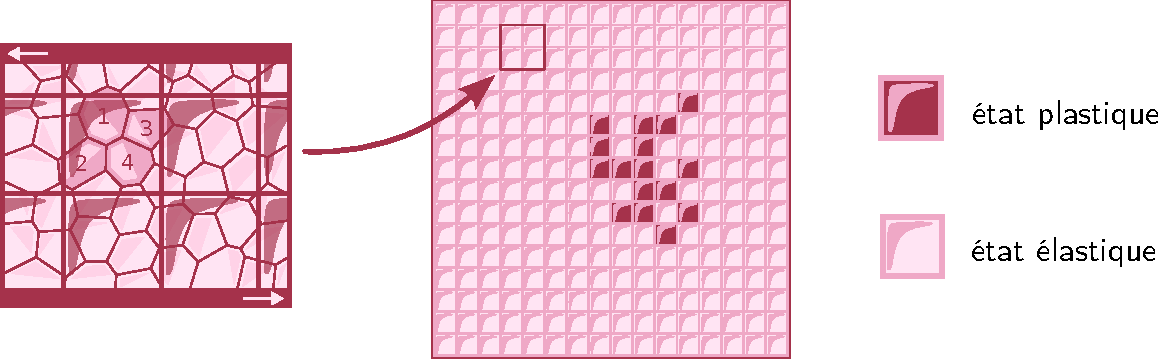
\includegraphics[width=0.8\textwidth]{Chapitre4/Figures/Methode/Mesoscaling.pdf}
	\caption{Représentation schématique du principe des modèles élastoplastiques. Chaque groupe de particules dans la vision microscopique est représenté par un site pouvant prendre deux états : élastique ou plastique.}
	\label{fig:mesoscale}
\end{figure}

\subparagraph{}Chaque site possède un seuil de contrainte microscopique local $\sigma_{Y,i}$ qu'il est capable de soutenir élastiquement. Mais dès lors que la contrainte locale excède ce seuil local ($\sigma_i > \sigma_{Y,i}$), le site devient à même d'opérer un réarrangement plastique. Ce processus intervient alors selon un temps caractéristique $\tau_{\text{pl}}$. Quand le réarrangement se produit, le site passe alors dans un état plastique ($n_i = 1$) et accumule une déformation plastique $\epsilon_{\text{pl},i}$ sur un temps caractéristique $\tau$. Cette déformation plastique permet alors une relaxation de la contrainte locale proportionnellement. La relaxation a lieu sur temps caractéristique $\tau_{\text{él}}$ après lequel le site retrouve son état élastique ($n_i = 0$).

\subparagraph{}Durant la relaxation, la contrainte accumulée par le site est redistribuée aux autres sites constituant le matériau via les interactions élastiques d'Eshelby, dont la forme est rappelée \autoref{fig:resultsimplem}-(a). Dans l'hypothèse que nous choisissons où les réarrangements plastiques présentent tous la même symétrie que le forçage, les propagateurs de Eshelby ont une orientation fixe, dans le sens du réseau. Cette redistribution va alors potentiellement permettre à d'autres sites de dépasser à leur tour leur seuil local et ainsi opérer un réarrangement. C'est cette interaction de redistribution et ces réarrangements en chaîne qui sont à l'origine du comportement collectif d'écoulement plastique du matériau.

\subparagraph{}Les règles précises qui définissent la co-évolution des variables $(\sigma_i, \epsilon_{\text{pl},i}, n_i)$ sur chaque site dépendent alors du modèle spécifique considéré.

\subsection{Le modèle de Picard}

\subparagraph{}Le modèle élastoplastique retenu pour mener notre étude est le modèle de Picard \cite{picard_slow_2005}. Ce modèle pionnier du domaine est reconnu pour sa simplicité. C'est alors un outil de choix pour étudier ce système du point de vue des transitions de phase absorbantes.

\subparagraph{}Dans le modèle de Picard, tous les sites composant le matériau, indicés $i$ et situés en $\mathbf{r}_i$, possèdent un seuil local identique et constant dans le temps $\sigma_{Y,i}=\sigma_Y$. Dès lors que son seuil est dépassé, un site devient plastique avec un taux de transition constant $1/\tau_ {\text{pl}}$. Une fois plastique, ce site retrouve sa forme élastique avec un taux $1/\tau_ {\text{él}}$. L'évolution de la contrainte locale d'un site isolé prend alors la forme illustrée sur la \autoref{fig:rules}.

\begin{figure}[h]
	\centering
	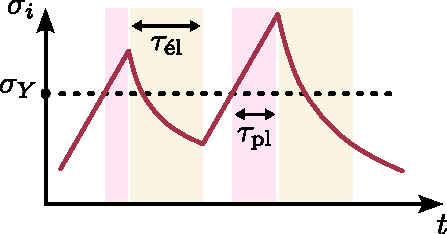
\includegraphics[width=0.5\textwidth]{Chapitre4/Figures/Methode/PicardTau.pdf}
	\caption{Représentation schématique de l'évolution de la contrainte locale dans le modèle de Picard pour un site isolé.}
	\label{fig:rules}
\end{figure}

\subparagraph{}Pour simplifier davantage cette approche, nous choisissons d'uniformiser les échelles de temps de telle manière que $\tau_{\text{pl}} = \tau_{\text{él}} = \tau$. On peut alors résumer ce modèle par le système d'équations suivant :

\begin{equation}
	\partial_t\sigma_i = 2\mu\sum_{j}G_{ij}\partial_t \epsilon_{pl,j},\quad \partial_t \epsilon_{pl,i} = \frac{1}{2\mu\tau}n_i \sigma_i,\quad
	\left\{
    \begin{array}{lcc}
    n_i: & 0\xrightarrow{\tau}1 & |\sigma_i|>\sigma_\mathrm{Y} \\
    n_i: & 0\xleftarrow{\tau}1 & \forall \sigma_i\\
    \end{array}
    \right.
\label{eq:PicardRules}
\end{equation}

\noindent avec $G_{ij} = G(\mathbf{r}_i-\mathbf{r}_j)$ le noyau de redistribution en champ lointain d'Eshelby  défini au \autoref{sec:introduction} et décrit en coordonées polaires par $G(r,\theta) = \frac{\cos 4\theta}{\pi r^2}$. Cette description peut aisément se généraliser en trois dimensions mais notre étude s'est concentrée uniquement sur le cas bidimensionnel. Afin de simplifier l'implémentation numérique, ce système d'équations est adimensionné par les transformations :

\begin{equation}
	\tilde{\sigma_i} = \frac{\sigma_i}{\sigma_Y},\quad \tilde{t} = \frac{t}{\tau}, \quad \tilde{\epsilon}_{pl,i} = \frac{\mu\tau}{\sigma_Y}\epsilon_{pl,i}
	\label{eq:PicardDim}
\end{equation}

\noindent pour obtenir :

\begin{equation}
	\partial_t\tilde{\sigma}_i = \sum_{j}G_{ij}\partial_t \tilde{\epsilon}_{pl,j},\quad \partial_t \tilde{\epsilon}_{pl,i} = n_i \tilde{\sigma}_i,\quad
	\left\{
    \begin{array}{lcc}
    n_i: & 0\xrightarrow{\tau}1 & |\tilde{\sigma}_i|>1 \\
    n_i: & 0\xleftarrow{\tau}1 & \forall \tilde{\sigma}_i\\
    \end{array}
    \right.
\label{eq:PicardRulesAdim}
\end{equation}

\noindent et nous omettrons le $\tilde{}$ pour alléger les notations dans la suite.

\subparagraph{}Il semble par ailleurs important de mentionner que la simplicité de ce modèle n'enlève rien à son pouvoir descriptif. En effet, pour les quantités et les phénomènes sur lesquels nous allons nous concentrer ici (exposants critiques, avalanches, ...) le modèle de Picard reproduit à l'identique les résultats des modèles plus raffinés \cite{ferrero_criticality_2019}, notamment ceux conservant une description tensorielle complète \cite{nicolas_deformation_2018, budrikis_universal_2017}.

\subsection{Implémentation numérique}

\subparagraph{}Afin de simuler l'écoulement cisaillé représenté par ce modèle, nous reprenons un code mis au point précédemment dans l'équipe PSM du LIPhy que nous modifions selon notre besoin. $N$ sites sont positionnés sur une grille carrée périodique de taille $L\times L = N$ et d'axes principaux $(\hat{\mathbf{e}}_x, \hat{\mathbf{e}}_y)$. La position de chaque site est alors donnée par $\mathbf{r}_i = na\hat{\mathbf{e}}_x + ma \hat{\mathbf{e}}_y$ avec $(n,m) \in \mathbb{N}^2$ et $a$ le pas du réseau que l'on prend égal à 1. En pratique, nous considérons la règle d'évolution directement sous sa forme intégrée :

\begin{equation}
	\sigma_i(t) = \sigma_{\text{int},i}(t)+\sigma_\text{ext} =  \sum_{j}G_{ij}\epsilon_{\text{pl},j}(t)+\Sigma
	\label{eq:DynPicardInteg}
\end{equation}

\noindent et l'évolution de $\epsilon_{\text{pl},j}$ donnée par l'\autoref{eq:PicardRulesAdim} est discrétisée dans le temps, calculée sur chaque site tous les $\Delta t = 10^{-2}~\tau$ selon une méthode d'Euler. \`A chaque pas de temps, les sites élastiques ($n_i=0$) au-dessus du seuil microscopique ($\sigma_i >1$) ont une probabilité $\Delta t / \tau$ de devenir plastiques tandis que les sites plastiques ont la même probabilité de redevenir élastiques.

\subparagraph{}Le point clé de l'algorithme est alors le calcul de la convolution $\sum_{j}G_{ij}\epsilon_{\text{pl},j}$ puisqu'elle admet naïvement une complexité d'ordre $N^2$. Afin d'optimiser nos calculs, nous tirons parti du fait que les sites soient disposés sur une grille régulière. Cela nous permet de déterminer ce terme selon une méthode pseudo-spectrale : la convolution est calculée dans l'espace de Fourier discret où elle devient le simple produit $\hat{G}(\mathbf{q})\hat{\epsilon}_{\text{pl}}(\mathbf{q})$ puis l'on revient à sa représentation dans l'espace réel par une transformée de Fourier inverse discrète. Pour ce faire, nous implémentons directement le propagateur de Eshelby dans sa forme spectrale discrète \cite{picard_elastic_2004} :

\begin{equation}
	\hat{G}(\mathbf{q}) = -4\frac{q_x^2 q_y^2}{q^4}, \quad (q_x, q_y) = \frac{2\pi}{L} \times (n,m)
	\label{eq:eshelbydiscretfourier}
\end{equation}

\noindent avec $\hat{G}(\mathbf{q}=0) = 0$ afin de conserver la contrainte totale du système. L'optimisation des algorithmes de FFT permet alors de réduire la complexité à l'ordre $N\log(N)$ \cite{cooley_algorithm_1965}. De plus, l'analyse de Fourier permet de prendre en compte les limites périodiques de manière naturelle. Le schéma de calcul devenant complètement parallélisable, il est implémenté sur des cartes graphiques via le langage CUDA \cite{cuda} afin d'optimiser nettement la rapidité d'exécution des simulations. Grâce à ces ajustements, nous sommes capables de simuler le comportement de systèmes dont la taille va de $L=32$ à $L=2048$\footnote{L'algorithme de FFT étant optimisé pour des tailles de la forme $2^n$ avec $n\in\mathbb{N}$, nous privilégions ces tailles pour les simulations.}.

\subparagraph{}En pratique, le système est d'abord cisaillé sous une forte contrainte globale $\Sigma_\text{preshear}$ durant un temps $T_\text{preshear}$ avant d'être soumis brutalement à la contrainte globale souhaitée $\Sigma$. Le système évolue alors jusqu'à un état stationnaire caractérisé par une valeur moyenne du taux de déformation $ \dot{\gamma}  = \frac{1}{N}\sum_{i}\partial_t\epsilon_{pl,i}$ (voir \autoref{fig:resultsimplem}-(b)), nulle pour $\Sigma<\Sigma_c$ et positive pour $\Sigma>\Sigma_c$. Nous sommes alors capables avec ce modèle de tracer la courbe d'écoulement $\langle \dot{\gamma} \rangle = f(\Sigma)$ représentée sur la \autoref{fig:resultsimplem}-(c), qui montre clairement la convexité de la transition, par opposition à la concavité de celle du dépiégeage. En étudiant le comportement du système pour $\Sigma \sim \Sigma_c$ il est alors possible de caractériser cette criticalité spécifique.

\begin{figure}[h]
	\centering
	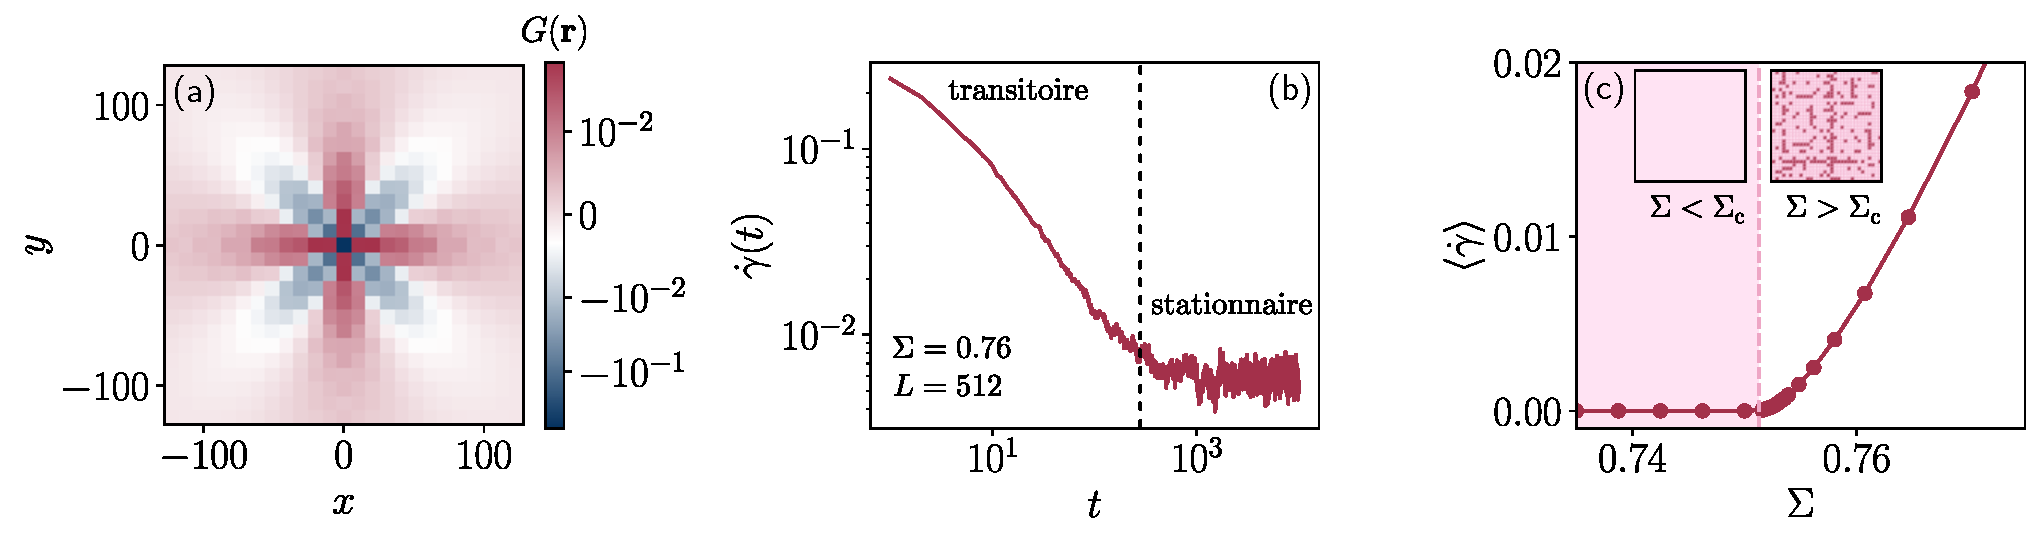
\includegraphics[width=\textwidth]{Chapitre4/Figures/Methode/ModeleResults.pdf}
	\caption{Résultats de l'implémentation numérique du modèle de Picard. (a) Image du propagateur de redistribution d'Eshelby. (b) Exemple d'équilibration d'une simulation à contrainte imposée. (c) Courbe d'écoulement pour un système de taille $L=256$.}
	\label{fig:resultsimplem}
\end{figure}

\subsection{Changement du paramètre de contrôle}

\label{sec:chgtcontrole}

\subparagraph{}De la même manière qu'il est possible de contrôler la contrainte globale à laquelle est soumis le système lors de la simulation, il est aussi possible de contrôler le taux de déformation $\dot{\gamma}$. Dans ce cas, les règles du modèle de Picard se voient légèrement modifiées \cite{picard_slow_2005}. Un terme de forçage  constant $\mu\dot{\gamma}$ s'ajoute à l'évolution de la contrainte locale dans l'\autoref{eq:PicardRules} et l'on a $\hat{G}^{\dot{\gamma}}(0) = -1$ de telle sorte que les évènements plastiques permettent une relaxation globale du système (et plus seulement locale) :

\begin{equation}
	\partial_t\sigma_i = \mu\dot{\gamma} + 2\mu\sum_{j}G^{\dot{\gamma}}_{ij}\partial_t \epsilon_{pl,j},\quad \partial_t \epsilon_{pl,i} = \frac{1}{2\mu\tau}n_i \sigma_i,\quad
	\left\{
    \begin{array}{lcc}
    n_i: & 0\xrightarrow{\tau}1 & |\sigma_i|>\sigma_\mathrm{Y} \\
    n_i: & 0\xleftarrow{\tau}1 & \forall \sigma_i\\
    \end{array}
    \right.
\end{equation}

\noindent Cette modification du propagateur n'est en fait pas simplement un artéfact numérique mais possède des origines physiques. Dans l'étude \cite{picard_elastic_2004}, Picard et al. ont montré que la forme précise du propagateur de Eshelby dépendait des conditions aux limites imposées (même lorsque celles-ci sont rejetées à l'infini), dépendant elles-mêmes du paramètre de contrôle associé. Dans le cas où les conditions aux limites conservent la contrainte dans le système, nous avons évidemment $\hat{G}(\mathbf{q}=0) = 0$. Par contre, dans le cas où les conditions aux limites imposent un déplacement, la contrainte globale n'est pas conservée et on a plus spécifiquement $\hat{G}^{\dot{\gamma}}(0) = -1$. Par contre pour $\mathbf{q}\neq 0$, les deux propagateurs de redistribution de la contrainte de cisaillement gardent la même forme.

\subparagraph{}De cette manière, il est possible d'appliquer un taux de déformation $\dot{\gamma}$ constant au système et d'observer l'évolution de la contrainte globale. Dans l'état stationnaire, cette dernière fluctue alors autour d'une valeur moyenne $\langle \Sigma\rangle$. Lorsque $\dot{\gamma}$ tend vers $0$, la contrainte moyenne tend vers la contrainte seuil $\Sigma_c$. Ce changement de paramètre de contrôle permet lui aussi d'observer le comportement du système et de tracer une courbe d'écoulement $\langle \Sigma \rangle = f(\dot{\gamma})$. On remarque par ailleurs que ces deux approches sont équivalentes sous cet aspect \cite{liu_driving_2016}.

\subparagraph{}Si la condition de contrainte imposée semble évidente dans le cas de l'étude de la transition de phase absorbante, contrôler le taux de déformation peut se révéler intéressant autant d'un point de vue numérique que du point de vue de la modélisation d'expériences réelles, comme nous le verrons par la suite.

\section{Comportement critique}

\rem{Citer plus ? Pourquoi ?}

\subparagraph{}Grâce au modèle de Picard, nous sommes donc en mesure de déterminer le comportement local et global du système proche du point critique $(\Sigma = \Sigma_c, \dot{\gamma} = 0)$. Des études basées sur une méthode élastoplastique similaire ont déjà permis d'analyser certaines propriétés critiques de la transition vers l'écoulement, comme les exposants critiques $\beta$ \cite{lin_scaling_2014, ferrero_criticality_2019, liu_driving_2016, jagla_different_2017} et $\nu_\perp$ \cite{lin_scaling_2014, korchinski_thermally_2024} ou encore ceux reliés aux propriétés d'avalanches du système \cite{liu_driving_2016, ferrero_criticality_2019, lin_scaling_2014, budrikis_universal_2017}, de manière similaire au cas de la transition de dépiégeage. Dans ce travail nous proposons une approche un peu différente en considérant une caractérisation dans la lignée directe de celles utilisées dans le cadre des transitions de phase absorbantes comme c'est le cas des modèles minimaux appartenant à la classe DP ou CDP.

\subsection{Transition vers l'écoulement en milieu élastique}

\subsubsection{Détermination du point critique}

\label{sec:methodepointcritique}

\paragraph{Méthodes}

\subparagraph{}Le première étape dans l'étude d'une transition de phase est la détermination de son point critique. Ici, cela revient à mesurer la contrainte seuil globale du système $\Sigma_c$. Pour ce faire plusieurs approches sont possibles.

\subparagraph{}La première approche consiste à reproduire la méthode appliquée dans les sections précédentes sur les modèles de particules. Cela revient ici à mesurer pour différentes contraintes imposées au système $\Sigma$ la valeur du taux de déformation moyen $\langle \dot{\gamma}\rangle$ dans l'état stationnaire. La contrainte seuil correspond alors à la contrainte pour laquelle la fonction $\langle \dot{\gamma} \rangle = f(\Sigma-\Sigma_c)$ est représentée par une droite sur une échelle logarithmique. Cette méthode, comme pour les modèles de particules, nécessite d'augmenter la taille du système $L$ à mesure que l'on s'approche du point critique et que l'activité dans le système (ici représentée par $\langle \dot{\gamma}\rangle$) s'approche de $0$.

\subparagraph{}La seconde méthode, plus communément utilisée dans la littérature, est de ne pas contrôler la contrainte imposée au système mais le taux de cisaillement (voir \autoref{sec:chgtcontrole}). De la même manière, la contrainte seuil est alors définie comme celle pour laquelle la fonction $\langle \Sigma \rangle - \Sigma_c = f(\dot{\gamma})$ est représentée par une droite sur une échelle logarithmique. L'avantage de ce choix est que lorsque le système est forcé, il ne peut jamais tomber dans l'état absorbant (puisque de fait $\dot{\gamma}>0$). Cela permet alors de s'affranchir du tâtonnement nécessaire à la première méthode. Toutefois cette méthode présente des inconvénients. En effet, si l'on peut imposer $\dot{\gamma}$ arbitrairement petit à n'importe quelle taille de système $L$, dès lors que la longueur de corrélation $\xi$ devient comparable à $L$, le système est soumis à des effets de taille finie. Ces effets parasitent alors la méthode de détermination graphique et incitent donc néanmoins à utiliser de plus grands systèmes à mesure que l'on s'approche du point critique.

\subparagraph{}Enfin, une troisième méthode astucieuse permet d'utiliser ces effets de taille finie afin de déterminer précisément $\Sigma_c$. Présentée dans \cite{lin_scaling_2014}, celle-ci consiste à soumettre le système à un cisaillement quasistatique selon un protocole qui sera développé à la \autoref{sec:imp_prot}. Pour chaque taille $L$ de système il est alors possible de mesurer la contrainte moyenne dans l'état quasistatique $\langle\Sigma_c (L)\rangle$. En supposant la correction de taille finie algébrique : $\langle\Sigma_c (L)\rangle = \Sigma_c+k_1 L^{-1/\nu_\perp}$, il est alors possible de déterminer graphiquement $\Sigma_c$. Le même raisonnement peut être effectué sur les fluctuations de cette contrainte en taille finie.

\subparagraph{}Les deux premières méthodes présentent l'avantage de déterminer conjointement $\Sigma_c$ et $\beta$, qui est un exposant d'intérêt principal pour nous. La troisième présente elle l'avantage de s'affranchir des effets parasites de taille finie. Toutefois, les deux dernières méthodes nécessitent la possibilité de changer de paramètre de contrôle (pour contrôler $\dot{\gamma}$ et non $\Sigma$). Elles sont donc facilement réalisables dans le cas des interactions élastiques avec $\alpha = 2$ mais, comme nous le verrons par la suite, cela devient moins évident dans le cadre d'une généralisation à des portées arbitraires. 

\paragraph{Détermination à taux de cisaillement imposé}

\label{sec:CP_Picard}

\subparagraph{}Pour l'analyse du cas élastique $\alpha = 2$, nous utilisons la deuxième méthode présentée. Pour des tailles de système $L \in [256, 512, 1024]$, nous réalisons des simulations à taux de cisaillement imposé. La mesure de $\langle \Sigma (\dot{\gamma},L)\rangle$ se fait une fois l'état stationnaire atteint. Les données associées aux trois systèmes sont alors assemblées et l'on trace la fonction $\dot{\gamma} = f(\langle \Sigma \rangle - \Sigma_c)$ en échelle logarithmique pour différentes valeurs de $\Sigma_c$. Comme illustré sur la \autoref{fig:CP_Classic}, $\Sigma_c=0.75125$ est une estimation convaincante de la contrainte seuil alors que $\Sigma_c^+=0.75130$ et $\Sigma_c^-=0.75120$ le sont moins. Moyennant les potentiels effets de taille finie entâchant la mesure, nous retiendrons $\Sigma_c=0.75125 \pm 0.00010$ comme détermination finale.

\begin{figure}[h]
	\centering
	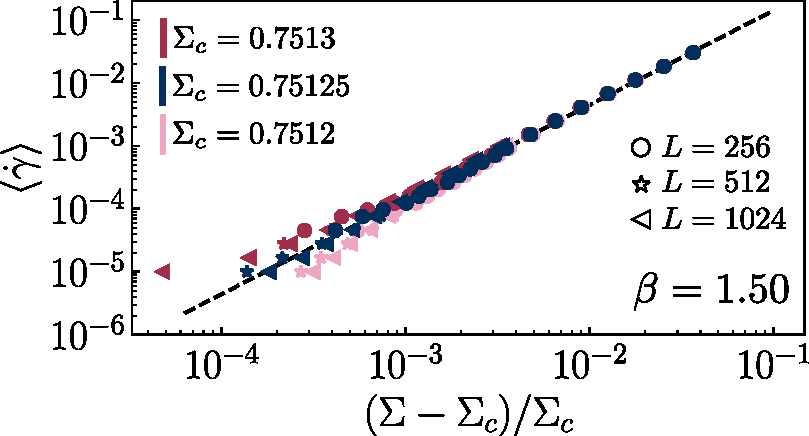
\includegraphics[width=0.65\textwidth]{Chapitre4/Figures/CasPhysique/CP_Classic.pdf}
	\caption{Détermination de la contrainte critique pour le modèle de Picard à taux de cisaillement imposé. La courbe en tirets noirs correspond à la loi de puissance $\langle\dot{\gamma}\rangle \sim \delta\Sigma^\beta$.}
	\label{fig:CP_Classic}
\end{figure}

\subparagraph{}Via cette détermination, la pente de la courbe donne directement $\beta=1.50 \pm 0.05$. Cette valeur est en parfait accord avec les résultats pré-existants sur les modèles élastoplastiques \cite{ferrero_criticality_2019, lin_scaling_2014}, confortant de ce fait la justesse de notre méthode de détermination. L'exposant $\beta$ mesuré est alors supérieur à 1, en accord avec les études précédentes, ce qui confirme bien que cette transition ne peut pas être décrite dans le cadre LR-CDP comme la transition de dépiégeage. De plus, cette valeur est différente de celle prédite par le modèle champ moyen généralement associé de Hébraud et Lequeux avec $\beta=2$ \cite{hebraud_mode-coupling_1998} et de sa généralisation dans le cas $\mu = D/\alpha = 1$ pour lequel on a $\beta = 1$ \cite{lin_mean-field_2016}. Afin de caractériser plus précisément la transition, nous déterminons dans la suite de cette section les autres exposants critiques associés.

\subsubsection{Analyse d'échelle de taille finie}

\paragraph{Difficultés dans la détermination des exposants critiques}

\subparagraph{}La détermination du point critique et de l'exposant $\beta$ est relativement coûteuse numériquement mais reste accessible. Pour les autres exposants $\gamma^\prime$ et $\nu_\perp$, celle-ci peut s'avérer plus fastidieuse. En effet, dans le cas de $\gamma^\prime$, la quantification précise de l'amplitude des fluctuations nécessite de plus longues simulations du fait qu'elles représentent un moment d'ordre supérieur de la distribution $P(\dot{\gamma})$. De plus le régime dans lequel $\langle\Delta\dot{\gamma}^2\rangle$ suit effectivement une loi de puissance est souvent plus réduit et demande donc une meilleure approche du point critique. Celle-ci ne peut se faire qu'en augmentant la taille du système et donc en allongeant de ce fait le temps de simulation. De plus, dans le cas de $\nu_\perp$, une mesure directe de la longueur de corrélation est fastidieuse du fait de l'anisotropie du modèle et de la longue portée des interactions \cite{liu_critical_2016}.

\paragraph{Méthode}

\label{sec:methodeFSS}

\subparagraph{}Afin de remédier à ces difficultés, nous proposons une méthode astucieuse inspirée des méthodes canoniques pour l'analyse des phénomènes critiques \cite{lubeck_universal_2004}. La difficulté première dans l'analyse de cette transition venant de la présence d'états absorbants, cette méthode permet de les supprimer. De la même manière que l'ajout d'un champ magnétique dans le modèle d'Ising permet de favoriser l'une des phases \cite{kardar_statistical_2007}, nous ajoutons au modèle un champ d'activation permettant de favoriser la phase active. En pratique, nous ajoutons une règle au modèle de Picard. Désormais, un site élastique peut devenir plastique peu importe sa contrainte locale. Cette nouvelle voie d'activation se fait selon un taux de transition $h$ qui représente alors l'intensité du champ d'activation :

\begin{equation}
n_i: 0\xrightarrow{h}1,\quad \forall \sigma_i \, .
\end{equation}

\subparagraph{}De ce fait, dès lors que $h>0$ le système ne peut pas tomber dans un état absorbant, quelque soit $\Sigma$. Cela revient à ajouter un paramètre de contrôle et donc une nouvelle dimension au diagramme critique, relocalisant le point critique en $(\Sigma = \Sigma_c, h=0)$, à la marge d'une zone non-absorbante (voir \autoref{fig:ChampAct}). En se plaçant à $\Sigma = \Sigma_c$ et $h>0$, faire tendre $h$ vers $0$ constitue ainsi un nouveau moyen de s'approcher du point critique sans aucun risque de tomber dans un état absorbant. En ce sens, imposer un champ d'activation $h$ est tout à fait analogue à imposer un taux de cisaillement $\dot{\gamma}$. Il est alors possible de sonder les propriétés critiques du système aussi près que l'on veut de la transition.

\begin{figure}
	\centering
	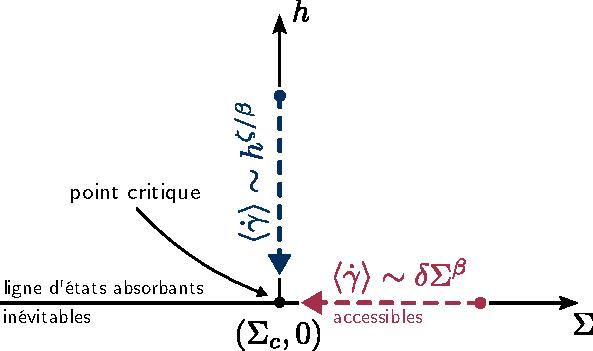
\includegraphics[width=0.6\textwidth]{Chapitre4/Figures/CasPhysique/ApprocheFSS.pdf}
	\caption{Représentation schématique du principe de l'ajout d'un champ d'activation $h$.}
	\label{fig:ChampAct}
\end{figure}

\subparagraph{}Néanmoins, comme dans le cas où l'on impose le taux de cisaillement $\dot{\gamma}$, dès lors que $\xi \sim L$ le système est soumis à des effets de taille finie. L'idée de l'analyse d'échelle en taille finie est alors de faire de ces effets de taille finie une force. Comme nous l'avons présenté au \autoref{chapter:introduction}, dans le régime critique et pour un système de taille infinie, les observables physiques sont des fonctions homogènes des paramètres de contrôle. En adaptant les notations au cas de la transition vers l'écoulement, cela signifie que l'on peut écrire $ \langle \dot{\gamma} \rangle$ comme :

\begin{equation}
\langle\dot{\gamma}\rangle \sim \lambda^{-\beta}R(a_\Sigma\lambda\delta\Sigma, a_h\lambda^\zeta h)
\end{equation}

\noindent avec $R$ une fonction universelle homogène de ses arguments, $a_i$ des paramètres non-universels et $\lambda > 0$. $\zeta$ représente alors un nouvel exposant critique caractérisant le champ d'activation $h$. En effet si l'on se place en $\Sigma = \Sigma_c$ et que l'on pose $\lambda=(a_h h)^{-1/\zeta}$ alors on obtient :

\begin{equation}
    \langle\dot{\gamma}\rangle \sim (a_h h)^{\beta/\zeta}R(0, 1)
\end{equation}

\noindent et donc $\langle\dot{\gamma}\rangle \sim  h^{\beta/\zeta}$. Afin d'intégrer les effets de taille finie dans cette description, nous considérons $L$ comme un nouveau paramètre de contrôle dont les propriétés d'échelle sont décrites par le même exposant $\nu_\perp$ que la longueur de corrélation $\xi$ :

\begin{equation}
    \langle\dot{\gamma}\rangle \sim \lambda^{-\beta}\tilde{R}(a_\Sigma \lambda\delta\Sigma,a_h\lambda^\zeta h, a_L L \lambda^{-\nu_\perp})
\end{equation}

\noindent En prenant alors $\Sigma=\Sigma_c$ et $\lambda=(a_LL)^{1/\nu_\perp}$ on obtient :

\begin{equation}
    \langle\dot{\gamma}\rangle \sim (a_LL)^{-\beta/\nu_\perp}\tilde{R}(0, a_h(a_LL)^{\zeta/\nu_\perp} h, 1)
\end{equation}

\subparagraph{}$\tilde{R}$ étant une fonction universelle, cela signifie qu'en redimensionnant $\langle\dot{\gamma}\rangle $ par $(a_LL)^{-\beta/\nu_\perp}$ et $h$ par $(a_LL)^{-\zeta/\nu_\perp}/a_h$, les courbes $\langle\tilde{\dot{\gamma}}\rangle = f(\tilde{h})$ ainsi représentées ne dépendent pas de la taille du système choisie. En des termes graphiques, les courbes obtenues pour différents $L$ se superposent, même au niveau des effets de taille finie. On peut alors établir une méthode graphique de détermination des exposants : en traçant les courbes $\langle \dot{\gamma} \rangle = f(h)$ pour différentes tailles $L$, les exposants critiques sont déterminés comme ceux définissant le redimensionnement permettant la superposition de toutes les courbes. En pratique, étant donné que cette étude ne sera menée que sur ce modèle spécifique, nous oublierons les paramètres non-universels $a_i$.

\subparagraph{}Ce raisonnement peut être mené sur deux autres quantités mesurables dans l'état stationnaire : la variance du taux de cisaillement global $\langle\Delta\dot{\gamma}^2\rangle$ et son cumulant de Binder $Q$ \cite{binder_finite_1981} défini selon :

\begin{equation}
    Q = 1 - \frac{\langle\dot{\gamma}^4\rangle}{3\langle\dot{\gamma}^2\rangle^2}
\end{equation}

\noindent L'universalité est alors obtenue avec le redimensionnement de $\langle\Delta\dot{\gamma}^2\rangle$ par $L^{\gamma^\prime/\nu_\perp}$ tandis que $Q$ ne nécessite pas de redimensionnement. La méthode que nous suivons pour la détermination des exposants est donc la suivante : 

\begin{itemize}
	\item par l'étude du cumulant $Q$ nous déterminons $\zeta/\nu_\perp$.
	\item par l'étude de $\langle\dot{\gamma}\rangle$ nous déterminons $\beta/\nu_\perp$.
	\item en utilisant la valeur mesurée de $\beta$ nous déduisons $\zeta$ et $\nu_\perp$.
	\item par l'étude de $\langle\Delta\dot{\gamma}^2\rangle$ nous déterminons $\gamma^\prime$.
\end{itemize}

\subparagraph{}Cette méthode peut en réalité être adaptée au cas similaire où le taux de cisaillement $\dot{\gamma}$ est imposé comme c'est le cas dans \cite{lin_scaling_2014}. Néanmoins notre méthode présente l'avantage de conserver la contrainte comme paramètre de contrôle et donc de permettre l'accès aux fluctuations du taux de cisaillement.

\paragraph{Résultats}

\subparagraph{}Nous simulons l'écoulement du système avec des tailles allant de $L=32$ à $L=1024$ et des valeurs de $h$ allant de $10^{-7}$ à $10^{-2}$. Dans les encarts de la \autoref{fig:FSS_Classic}, nous observons alors le comportement typique attendu du système en présence d'effets de taille finie. Loin du point critique où la longueur de corrélation $\xi$ est grande devant $L$, toutes les courbes suivent une même évolution (partie droite des encarts). En revanche, en s'approchant du point critique, en diminuant $h$, les effets de taille finie se ressentent d'autant plus tôt que la taille du système $L$ est petite, induisant un décrochage de la loi universelle (partie gauche des encarts).



\subparagraph{}En appliquant la méthode décrite précédemment, il est possible d'obtenir la meilleure estimation des exposants $\zeta$, $\nu_\perp$ et $\gamma^\prime$ grâce aux superpositions de courbes représentées à la \autoref{fig:FSS_Classic}. La justesse des superpositions obtenues valide notre approche d'échelle et  nous permet d'obtenir des estimations plus précises que via une méthode d'ajustement classique. Les valeurs des exposants sont alors reportées dans le \autoref{tab:expocrit}. Notons que si cette transition est largement étudiée, la valeur des exposants $\gamma^\prime$ et $\zeta$ n'avait encore jamais été déterminée puisque les études précédentes adoptent un point de vue plutôt centré sur la rhéologie associée que sur la caractérisation théorique en tant que transition de phase absorbante.

\begin{figure}[h]
	\centering
	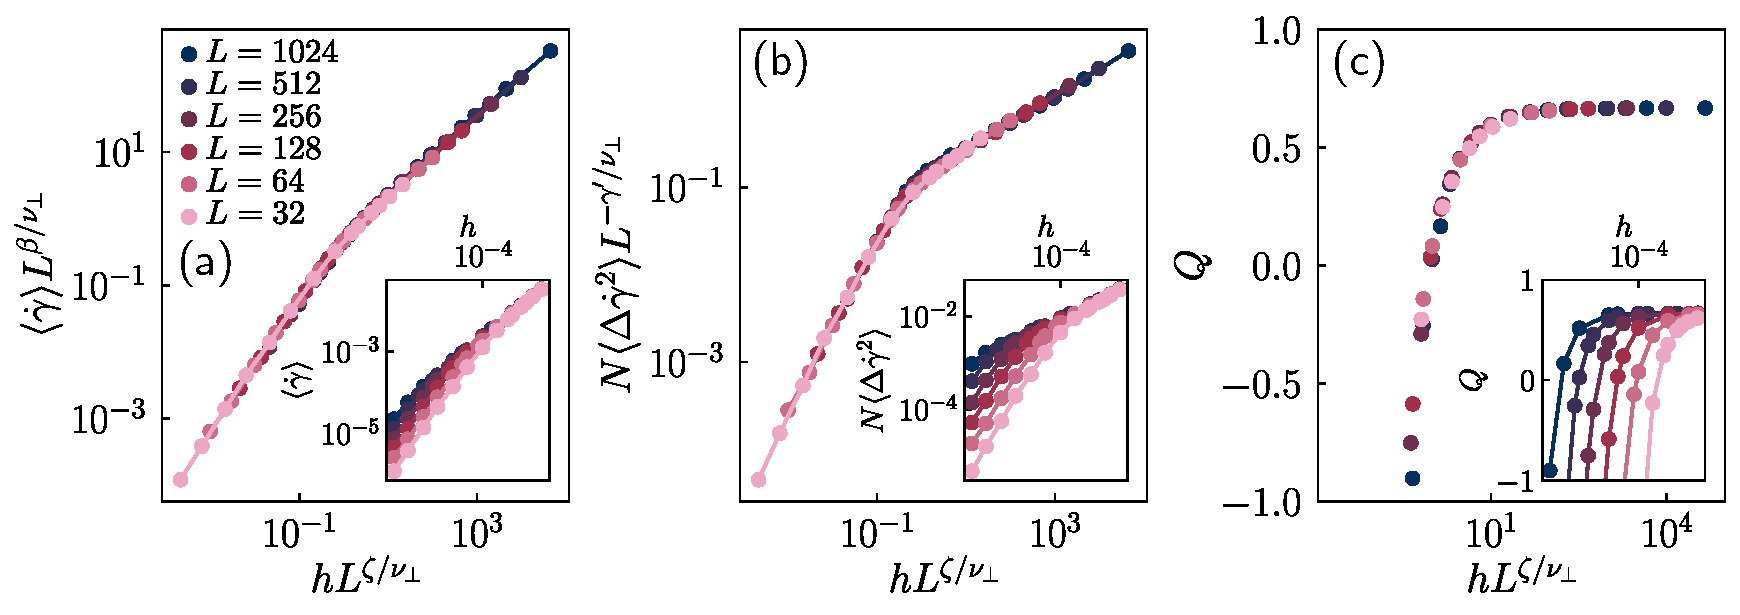
\includegraphics[width=\textwidth]{Chapitre4/Figures/CasPhysique/FSS_Classic_edited.pdf}
	\caption{Analyse d'échelle de taille finie pour le modèle de Picard. Redimensionnement de l'évolution de (a) la valeur moyenne du taux de cisaillement, (b) de la variance taux de cisaillement, (c) du cumulant de Binder. En encart, nous représentons les données brutes avant redimensionnement.}
	\label{fig:FSS_Classic}
\end{figure}

\subparagraph{}La valeur de l'exposant lié à la longueur de corrélation $\nu_\perp \approx 1.13$ est en accord avec celle trouvée dans le cas d'un autre modèle élastoplastique \cite{lin_scaling_2014}.

\begin{table}
\centering
\begin{tabular}{ccccc}
\hline \hline Modèle/Classe & $\beta$ & \multicolumn{1}{c}{$\gamma^{\prime}$} & $\nu_{\perp}$ & $\zeta$ \\
\hline Picard & 1.5 & -0.70 & 1.1 & 2.5 \\
Picard-CP & 0.59 & 0.26 & 0.70 & 2.1 \\
$\text{FES}^\pm$ & 0.62 & 0.36 & 0.79 & 2.25 \\
CDP \cite{lubeck_universal_2004} & 0.64 & 0.37 & 0.80 & 2.23 \\
\hline \hline
\end{tabular}
\caption{Exposants critiques déterminés dans le modèle de Picard, le modèle Picard-CP, le modèle $\text{FES}^\pm$ et les exposants attendus pour la classe CDP.}
\label{tab:expocrit}
\end{table}

\subsubsection{Relation d'hyperscaling}

\subparagraph{}L'exposant lié aux fluctuations critiques prend lui une valeur $\gamma^\prime \approx -0.7$, elle aussi exclue du cadre théorique LR-CDP pour lequel on a nécessairement $\gamma^\prime>0$. Le point le plus intéressant est que cette valeur est négative. Cela signifie que lorsque l'on approche la contrainte seuil du système, les fluctuations du taux de déformation diminuent et finissent par s'annuler complètement au point critique exactement. Ce comportement est assez contre-intuitif de prime abord. En effet, du fait du renforcement des corrélations spatiales et temporelles à l'approche du point critique, le scénario habituel des phénomènes critiques présente des fluctuations critiques qui, au contraire, divergent \cite{kardar_statistical_2007}. Cette observation surprenante permet néanmoins de satisfaire la relation d'hyperscaling introduite au \autoref{chapter:introduction} :

\begin{equation}
	\gamma^\prime = \nu_\perp D - 2\beta
	\label{eq:hyperscalingEPM}
\end{equation}

\noindent pour laquelle on trouve ici $(2\beta + \gamma^\prime) / \nu_\perp D\approx 1.01$.  

\subparagraph{}Cette dernière peut en fait être rationalisée par un scénario simple dans le cas de la transition vers l'écoulement. Dans l'état stationnaire, le système peut être vu comme une collection de $(L/\xi)^D$ sous-systèmes indépendants de taille $\xi \times \xi$. Conforté par le scénario proposé dans \cite{lin_scaling_2014}, dans chaque compartiment le taux de cisaillement moyen $\langle\dot{\gamma}\rangle_\xi$ est imposé par celui produit par les plus grands évènements, ici d'extension spatiale $\xi$. Les compartiments étant indépendants, chacun d'entre eux possède un taux de cisaillement moyen égal au taux de cisaillement moyen global du système $\langle \dot{\gamma} \rangle$. En supposant alors que la durée des évènements et leur période d'apparition suivent les mêmes lois d'échelles, la variance du taux de cisaillement dans chaque compartiment, qui est une quantité positive, se comporte comme le carré du taux de cisaillement moyen $\langle \Delta\dot{\gamma}^2 \rangle_\xi \sim \langle\dot{\gamma}\rangle_\xi^2 \sim \langle\dot{\gamma}\rangle^2$. La variance globale $\langle \Delta\dot{\gamma}^2 \rangle$ est alors l'addition de celle de tous les compartiments indépendants :

\begin{equation}
	\langle \Delta\dot{\gamma}^2 \rangle \sim \left(\frac{L}{\xi}\right)^D\langle \Delta\dot{\gamma}^2 \rangle_\xi \sim \left(\frac{L}{\xi}\right)^D\langle \dot{\gamma} \rangle^2
\end{equation}

\noindent ce qui permet d'arriver à la relation d'hyperscaling en ré-exprimant toutes les grandeurs en fonction de la distance au point critique $\delta\Sigma$. En d'autres termes, l'évolution des fluctuations du taux de cisaillement est le fruit de deux phénomènes en compétition. D'une part à l'approche de la transition le nombre de zones indépendantes spatialement diminue, augmentant de ce fait les fluctuations globales (terme $\nu_\perp D$ dans l'équation \autoref{eq:hyperscalingEPM}). D'autre part le taux de cisaillement moyen, et donc sa variance, diminue dans chacune de ces zones à l'approche du point critique (terme $-2\beta$ dans l'équation \autoref{eq:hyperscalingEPM}). Dès lors que l'exposant $\beta$ est suffisamment grand, l'exposant $\gamma^\prime$ est donc susceptible de devenir négatif, ce qui est bien le cas ici.

\subparagraph{}Cette image n'est cependant pas en contradicition avec des fluctuations relatives de plus en plus grandes à l'approche du point critique, puisque $\langle \Delta\dot{\gamma}^2 \rangle/\langle \dot{\gamma}\rangle^2 \sim \delta\Sigma^{-\gamma^\prime - 2\beta}$ et $-\gamma^\prime - 2\beta < 0$. Ainsi, si les fluctuations absolues du taux de cisaillement s'annulent à l'approche du point critique, les fluctuations relatives, elles, divergent bien.

\subsection{Modèles d'écoulement à courte portée}

\subparagraph{}Grâce au modèle de Picard, nous avons donc pu estimer les exposants critiques liés à la transition vers l'écoulement dans le cas physique d'interactions élastiques pour lesquelles on a $\alpha = 2$. Afin de resituer cette transition dans une image plus globale, nous proposons de caractériser son évolution en fonction de la portée des interactions qu'elle met en oeuvre. Pour commencer, nous nous concentrons sur le cas limite de courte portée.

\subsubsection{Le modèle Picard-CP}

\subparagraph{} Pour ce faire, nous produisons la même analyse mais sur une variation du modèle de Picard que l'on nommera Picard-CP pour "Picard courte portée". Le modèle Picard-CP reprend alors toutes les règles du modèle de Picard mais considère une interaction différente. Celle-ci porte uniquement sur les premiers voisins, supprimant ainsi tous les effets de la longue portée de l'interaction. Pour conserver toutes choses égales par ailleurs, le noyau de redistribution choisi conserve la symétrie particulière du noyau d'Eshelby et prend donc la forme décrite sur la \autoref{fig:Prog_CP_SR}-(a). Nous nous attendons alors à ce que ce modèle appartienne à la classe CDP puisqu'il ressemble fortement à un modèle de tas de sables, comme le modèle Manna. Nous rappelons que cette classe d'universalité est décrite par les exposants récapitulés dans le \autoref{tab:expocrit}.

\subparagraph{}Pour déterminer la contrainte critique associée à ce nouveau modèle, nous utilisons la méthode de contrainte imposée présentée à la \autoref{sec:methodepointcritique}. Dans ce cas, il n'y a en fait aucune manière naturelle de changer le paramètre de contrôle du système pour contrôler le taux de cisaillement. En effet, cela demanderait d'ajouter une composante de relaxation globale au noyau de redistribution qui peut alors prendre n'importe quelle forme (uniforme, locale, ...), et qui a priori ne donnera pas la même courbe d'écoulement que dans des conditions de contrainte imposée. En utilisant des systèmes de tailles allant de $L=256$ à $L=1024$, nous obtenons les résultats présentés sur la \autoref{fig:Prog_CP_SR}-(b), permettant de déterminer la contrainte seuil comme étant $\Sigma_c = 0.75433 \pm 0.00005$ et l'exposant $\beta = 0.59 \pm 0.02$. On trouve alors une courbe d'écoulement concave ($\beta < 1$), plus communément attendue dans le cadre des phénomènes critiques. Un point à noter est que la détermination du point critique se révèle ici beaucoup plus simple que dans le cas physique en termes de temps de calcul. Cela vient directement du caractère concave de la transition qui permet de s'approcher tout aussi près du point critique sans pour autant avoir à descendre à des taux de cisaillement extrêmement faibles et donc aller à des tailles de système extrêmement grandes.

\begin{figure}[h]
	\centering
	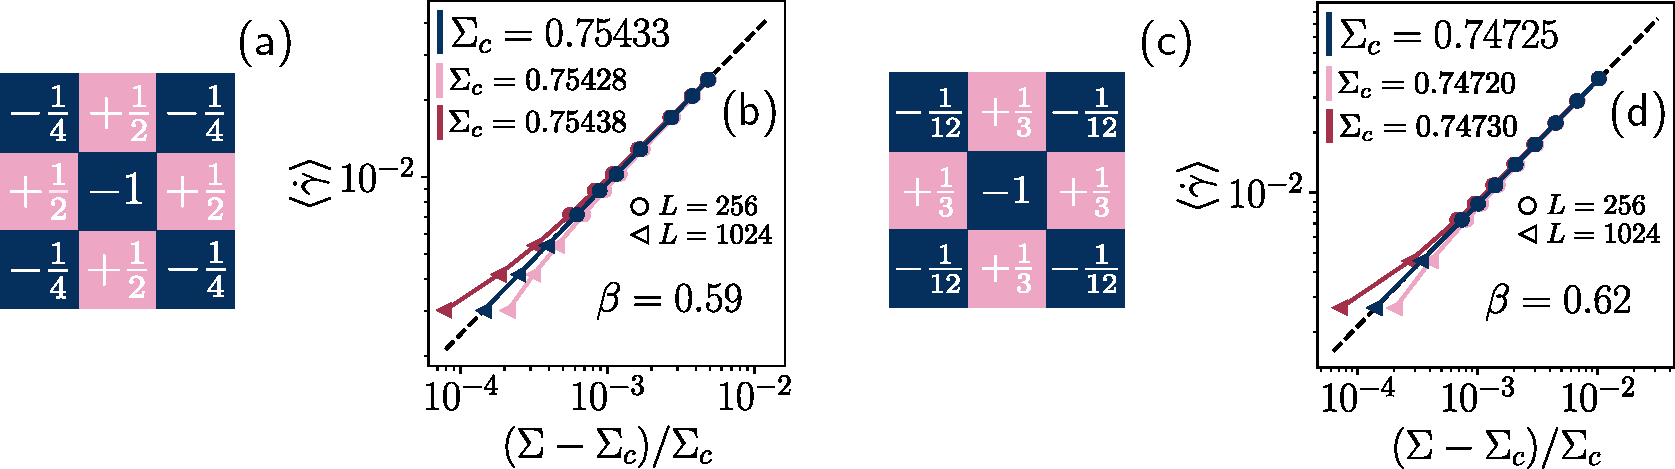
\includegraphics[width=\textwidth]{Chapitre4/Figures/CourtePortee/Prog_CP.pdf}
	\caption{Détermination de la contrainte critique $\Sigma_c$ et de l'exposant $\beta$ pour le modèle Picard-CP (b) (dont le propagateur est représenté en (a)) et pour le modèle $\text{FES}^\pm$ (c) (dont le propagateur est représenté en (d))}
	\label{fig:Prog_CP_SR}
\end{figure}

\subparagraph{}La valeur obtenue de l'exposant $\beta$ est alors très proche de celle attendue pour la classe CDP, même si la mesure numérique semble s'en éloigner très légèrement. Cet écart n'est pas non plus dérisoire puisque c'en est un du même ordre de grandeur qui permet de séparer les classes DP et CDP par exemple \cite{lubeck_universal_2004}. Afin de confirmer ou réfuter l'hypothèse que CDP, comme pour la transition de dépiégeage, est la classe représentant le modèle Picard-CP, nous le caractérisons grâce à une analyse d'échelle de taille finie. En simulant des systèmes pour des tailles allant de $L=32$ à $L=512$, la meilleure superposition des courbes après redimensionnement est représentée \autoref{fig:FSS_SRP}-(a)-(c). Les valeurs des exposants critiques estimées sont alors reportées dans le \autoref{tab:expocrit}.

\begin{figure}[h]
	\centering
	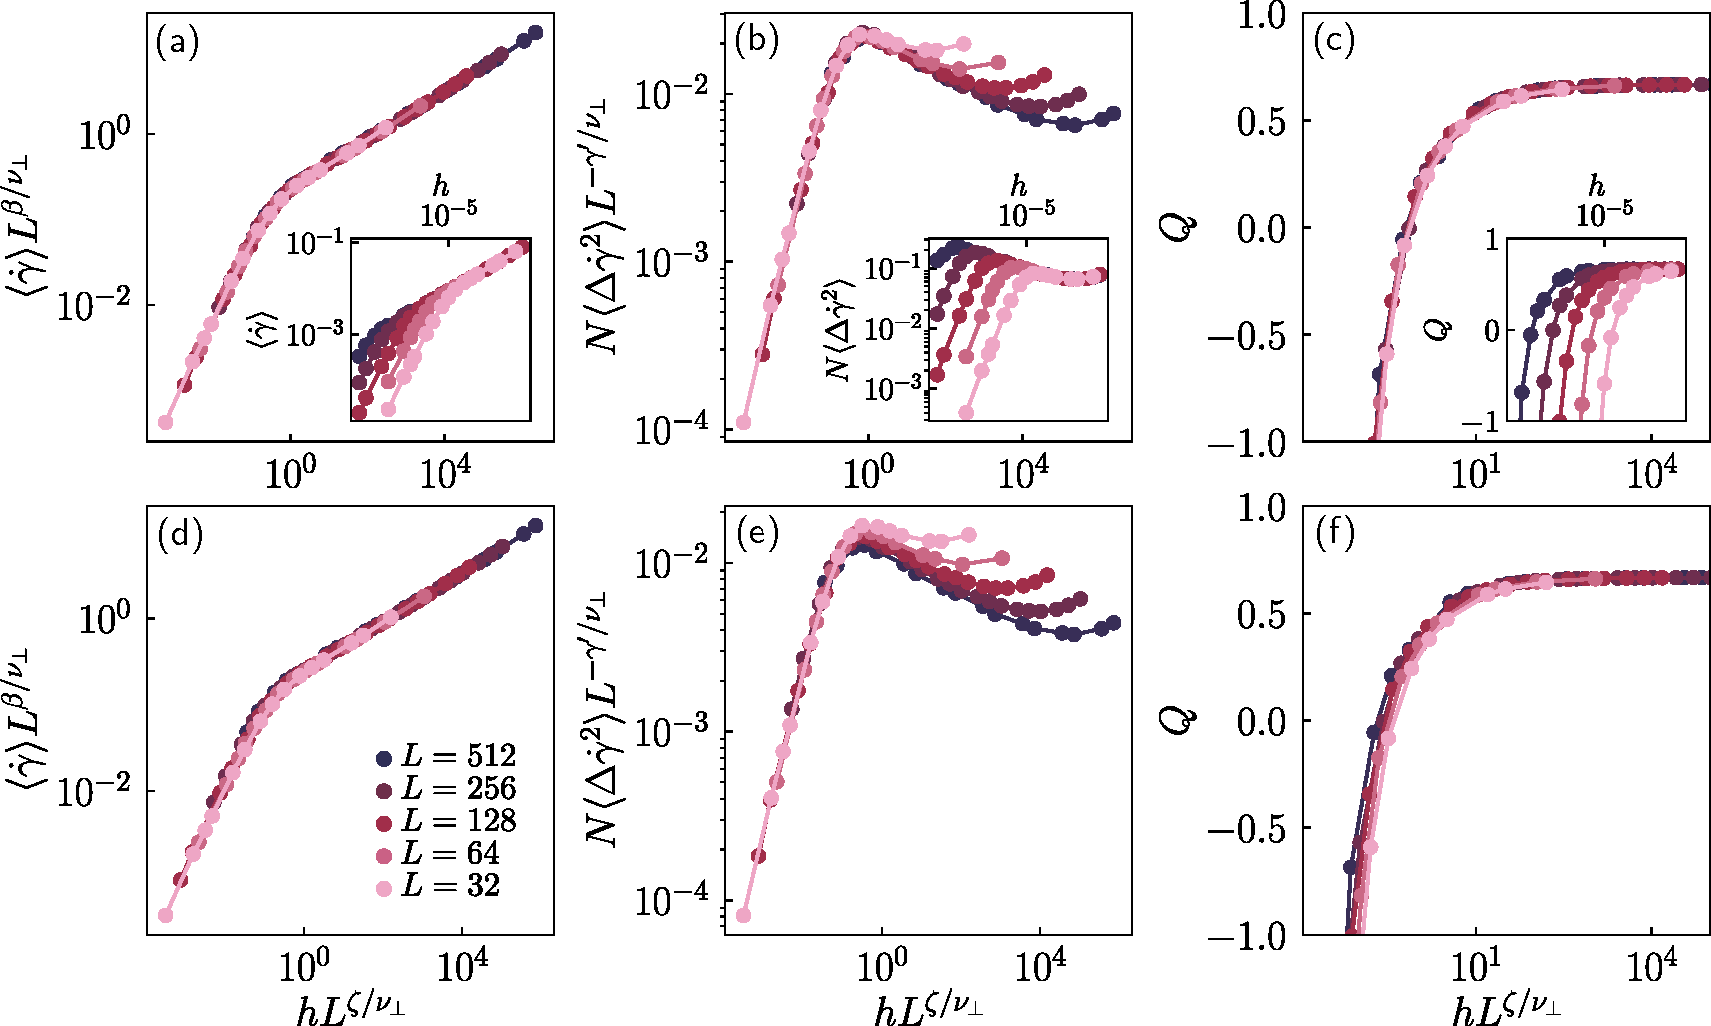
\includegraphics[width=\textwidth]{Chapitre4/Figures/CourtePortee/FSS_SRP_edited.pdf}
	\caption{Analyse d'échelle de taille finie dans le cas du modèle Picard-CP. Les redimensionnements de la valeur moyenne (a), de la variance (b) et du cumulant de Binder (c) du taux de cisaillement sont représentés en figures principales et les données brutes en inset. Les figures (d), (e) et (f) montrent ces mêmes redimensionnement avec les exposants connus de la classe CDP \cite{lubeck_universal_2004}.}
	\label{fig:FSS_SRP}
\end{figure}

\subparagraph{} La première observation à faire est que l'exposant lié aux fluctuations $\gamma^\prime \approx 0.26$ est positif. On retrouve donc le comportement canonique des fluctuations critiques qui divergent à l'approche de la transition, conjointement au fait de retrouver une valeur de l'exposant $\beta$ relativement petite. Par ailleurs, avec la valeur mesurée plus faible de l'exposant $\nu_\perp \approx 0.7$, la relation d'hyperscaling est encore une fois très bien vérifiée avec $(2\beta + \gamma^\prime)/\nu_\perp D \approx 1.03$. Le scénario proposé à la section précédente est donc toujours envisageable, mais le terme $2\beta$ subit une variation plus importante que le terme $\nu_\perp D$ ce qui inverse le rapport de force entre les deux phénomènes en compétition.

\subparagraph{}Par ailleurs, les exposants $\nu_\perp$, $\zeta$ et $\gamma^\prime$ prennent eux aussi des valeurs proches des valeurs attendues pour la classe CDP, mais semblent pourtant discernablement différents. Pour se convaincre de cette différence, nous utilisons les exposants associés à la classe CDP pour la procédure de redimensionnement. Si cette classe est bien la représentante du modèle, alors la superposition dans ce cas devrait être au moins aussi convaincante. La superposition des courbes obtenue dans ce cas est présentée sur la \autoref{fig:FSS_SRP}-(d)-(f). On remarque alors que celle-ci est de qualité bien moindre, notamment dans le cas de la variance et du cumulant de Binder. En effet, la zone de changement de tendance pour la variance (i.e. la bosse présentée sur la \autoref{fig:FSS_SRP}-(e)) marque un désaccord entre les différentes courbes tandis que la superposition des cumulants $Q$ est relativement mauvaise à petits $h$. Les exposants précédemment estimés permettant d'améliorer fortement ces désaccords, cette analyse suggère que le modèle Picard-CP n'appartient pas à la classe d'universalité CDP. Cela peut paraître surprenant car toutes les conditions de la conjecture de Rossi et. al \cite{rossi_universality_2000} semblent être réunies ici.

\subsubsection{Modes zéros, propriété fondamentale de la transition vers l'écoulement}

\subparagraph{}Si le modèle fait bien intervenir une infinité d'états absorbants, des interactions à courte portée et une quantité conservée, il n'est pas dépourvu de symétrie supplémentaire. En effet, si l'on se penche sur la structure du noyau de redistribution, on remarque que la somme des contributions sur chaque ligne et chaque colonne est nulle (voir \autoref{fig:Omodesshortrange}-(a)). Cette symétrie n'est pas anodine puisqu'elle implique qu'au cours de l'écoulement la contrainte portée par une ligne ou une colonne est conservée. Le système n'est donc pas contraint uniquement par la conservation de la contrainte globale mais aussi par celle de $2L$ contraintes partielles. En espace de Fourier, cette symétrie correspond à $\hat{G}(q_x=0,q_y)=\hat{G}(q_x,q_y=0)=0$, qui est bien apparente dans le cas du modèle Picard-CP où l'on a :

\begin{equation}
	\hat{G}(\mathbf{q}) = \cos(q_x) + \cos(q_y) -\cos(q_x)\cos(q_y) -1
\end{equation}

\begin{figure}[h]
	\centering
	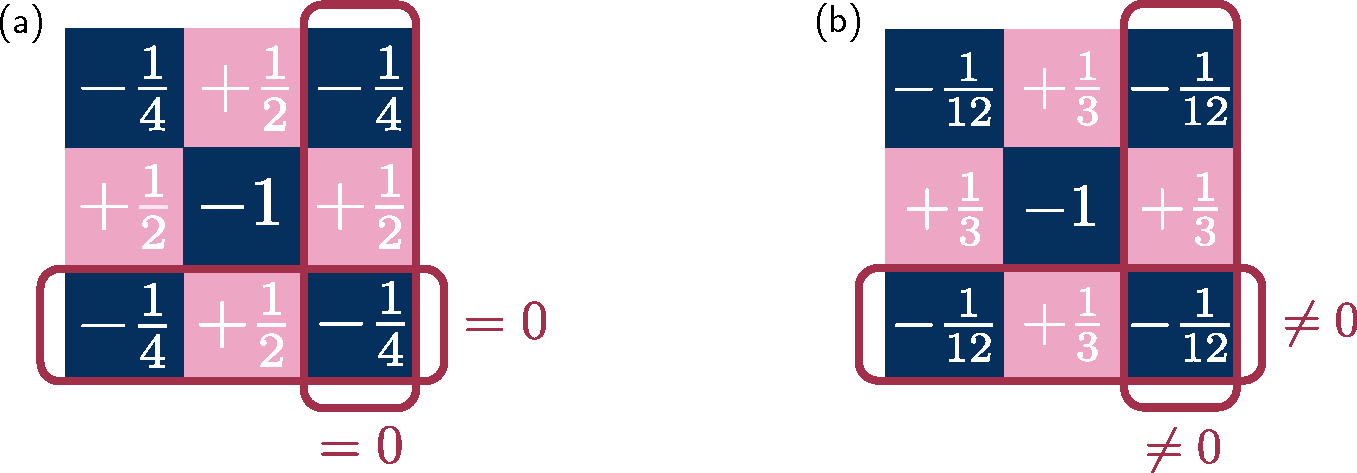
\includegraphics[width = 0.8\textwidth]{Chapitre4/Figures/CourtePortee/ZMCP.pdf}
	\caption{Illustration de la propriété de mode zéro dans le cas du modèle Picard-CP (a) et sa brisure dans le cas du modèle $\text{FES}^\pm$ (b)}
	\label{fig:Omodesshortrange}
\end{figure}

\subparagraph{}Cette propriété est en fait une propriété déjà connue et étudiée dans le cas classique \cite{tyukodi_depinning_2016, ferrero_elastic_2019}. En effet, d'après l'\autoref{eq:eshelbydiscretfourier} on a de même pour l'interaction d'Eshelby $\hat{G}(q_x=0,q_y)=\hat{G}(q_x,q_y=0)=0$. Cette conservation supplémentaire peut être interprétée sous un autre angle. Si un évènement plastique ne modifie pas la contrainte partielle portée par chaque ligne et colonne, alors une ligne ou colonne d'évènements ne modifie pas l'état de contrainte locale du système. En termes de physique d'équilibre, si l'on s'accorde ce parallèle, ces lignes plastiques ont un coût énergétique nul et peuvent donc être qualifiées de "modes mous". C'est cette propriété qui explique pourquoi ce système, proche du point critique, présente une activité plastique organisée sous forme de clusters de faible compacité, presque linéaires (voir \autoref{fig:FractalDim}). Les bandes de cisaillement \cite{martens_spontaneous_2012, rossi_finite-disorder_2022} sont alors la représentation à son paroxysme de cette symétrie. Ces corrélations observées dans différents dispositifs expérimentaux montrent par ailleurs que cette propriété n'est pas uniquement un artefact numérique mais a un impact bien réel sur la physique du phénomène d'écoulement. Par analogie avec les modes mous de la physique d'équilibre et la condition dans l'espace de Fourier, nous appellerons ces modes de plasticité "modes zéros". 

\begin{figure}[h]
	\centering
	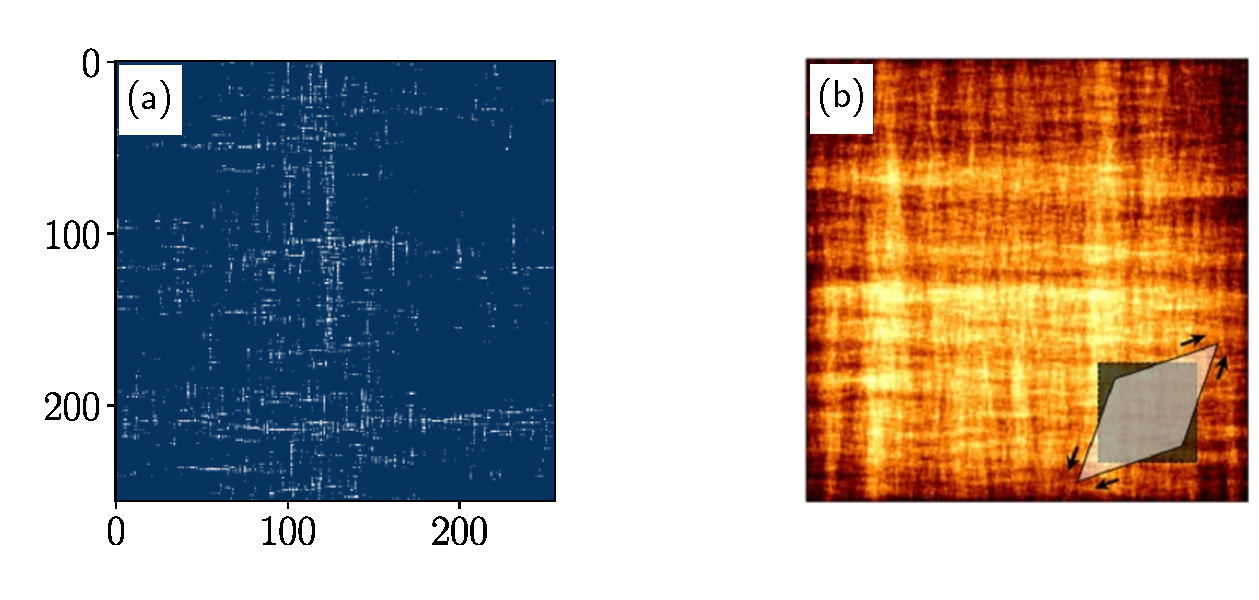
\includegraphics[width=0.8\textwidth]{Chapitre4/Figures/CourtePortee/StrainLoc.pdf}
	\caption{(a) Carte d'activité plastique cumulée au cours d'une simulation du modèle de Picard. Les zones blanches représentent des zones de forte activité plastique. (b) Même carte dans le cas d'un modèle élastoplastique tensoriel implémenté par une méthode d'éléments finis \cite{budrikis_universal_2017}}
	\label{fig:FractalDim}
\end{figure} 

\subparagraph{}Dans le cas classique, cette propriété de modes zéros qui se retrouve dans le noyau d'Eshelby n'est pas un hasard. En effet, elle vient du fait que l'interaction considérée est regardée dans la théorie de l’élasticité linéaire à l'équilibre mécanique. Cela implique donc que la divergence du tenseur des contraintes est nulle à tout moment de l'écoulement :

\begin{equation}
	\partial_i\sigma_{ij} = 0 \Rightarrow \left\{
    \begin{array}{lccc}
    \partial_x \sigma_{xx} & +& \partial_y \sigma_{yx} & =0 \\
    \partial_y \sigma_{yy} & +& \partial_x \sigma_{xy} & =0 \\
    \end{array}
    \right.
\end{equation}

\noindent En intégrant alors sur $x$ la première équation et sur $y$ la seconde, et en se rappelant que $\sigma_{xy} = \sigma_{yx}$ on a :

\begin{equation}
	\partial_x \int \mathrm{d}y~ \sigma_{xy} = \partial_y \int \mathrm{d}x~ \sigma_{xy} = 0
\end{equation}

\noindent ce qui implique que la contrainte partielle portée par chaque ligne et colonne est la même. Le propagateur de redistribution d'Eshelby qui répond à cette contrainte d'équilibre mécanique doit donc redistribuer la même contrainte partielle sur chaque ligne et colonne. De plus, étant de moyenne nulle afin de conserver la contrainte globale, cette contrainte partielle redistribuée est nécessairement nulle.

\subsubsection{Retour à l'universalité et classe CDP-0}

\label{sec:continuCDP0}

\subparagraph{}Afin de confirmer l'hypothèse que le modèle Picard-CP ne tombe pas dans la classe CDP du fait de la présence de modes zéros, nous étudions une troisième variation du modèle. Tout en conservant les mêmes règles par ailleurs, le noyau d'interaction sur les plus proches voisins est modifié de sorte que les modes zéros disparaissent (voir \autoref{fig:Omodesshortrange}). Ceci se fait tout en gardant la symétrie quadrupolaire de l'interaction et donc des signes alternés. En ce sens, nous appelons ce modèle $\text{FES}^\pm$ du fait de sa forte ressemblance avec les modèles de tas de sable à énergie conservée (\textit{fixed-energy sandpiles}) mais qui ne présentent en général que des redistributions de masse positives.

\subparagraph{}Nous déterminons alors le point critique associé à ce modèle de la même manière que pour le précédent. Les résultats présentés sur la \autoref{fig:Prog_CP_SR}-(c) donnent $\Sigma_c \approx 0.74725 \pm 0.00005$ et $\beta = 0.62 \pm 0.02$. On remarque alors d'abord un accord légèrement meilleur avec l'exposant $\beta$ attendu pour la classe CDP. Afin de confirmer ce rapprochement, nous conduisons la même analyse d'échelle de taille finie. Les résultats obtenus pour le meilleur redimensionnement sont présentés \autoref{fig:FSS_SRNC}-(a)-(c). Les exposants $\nu_\perp$, $\zeta$ et $\gamma^\prime$ ont alors des valeurs estimées toutes plus proches des valeurs attendues pour la classe CDP que dans le cas du modèle Picard-CP (voir \autoref{tab:expocrit}). 

\begin{figure}[h]
	\centering
	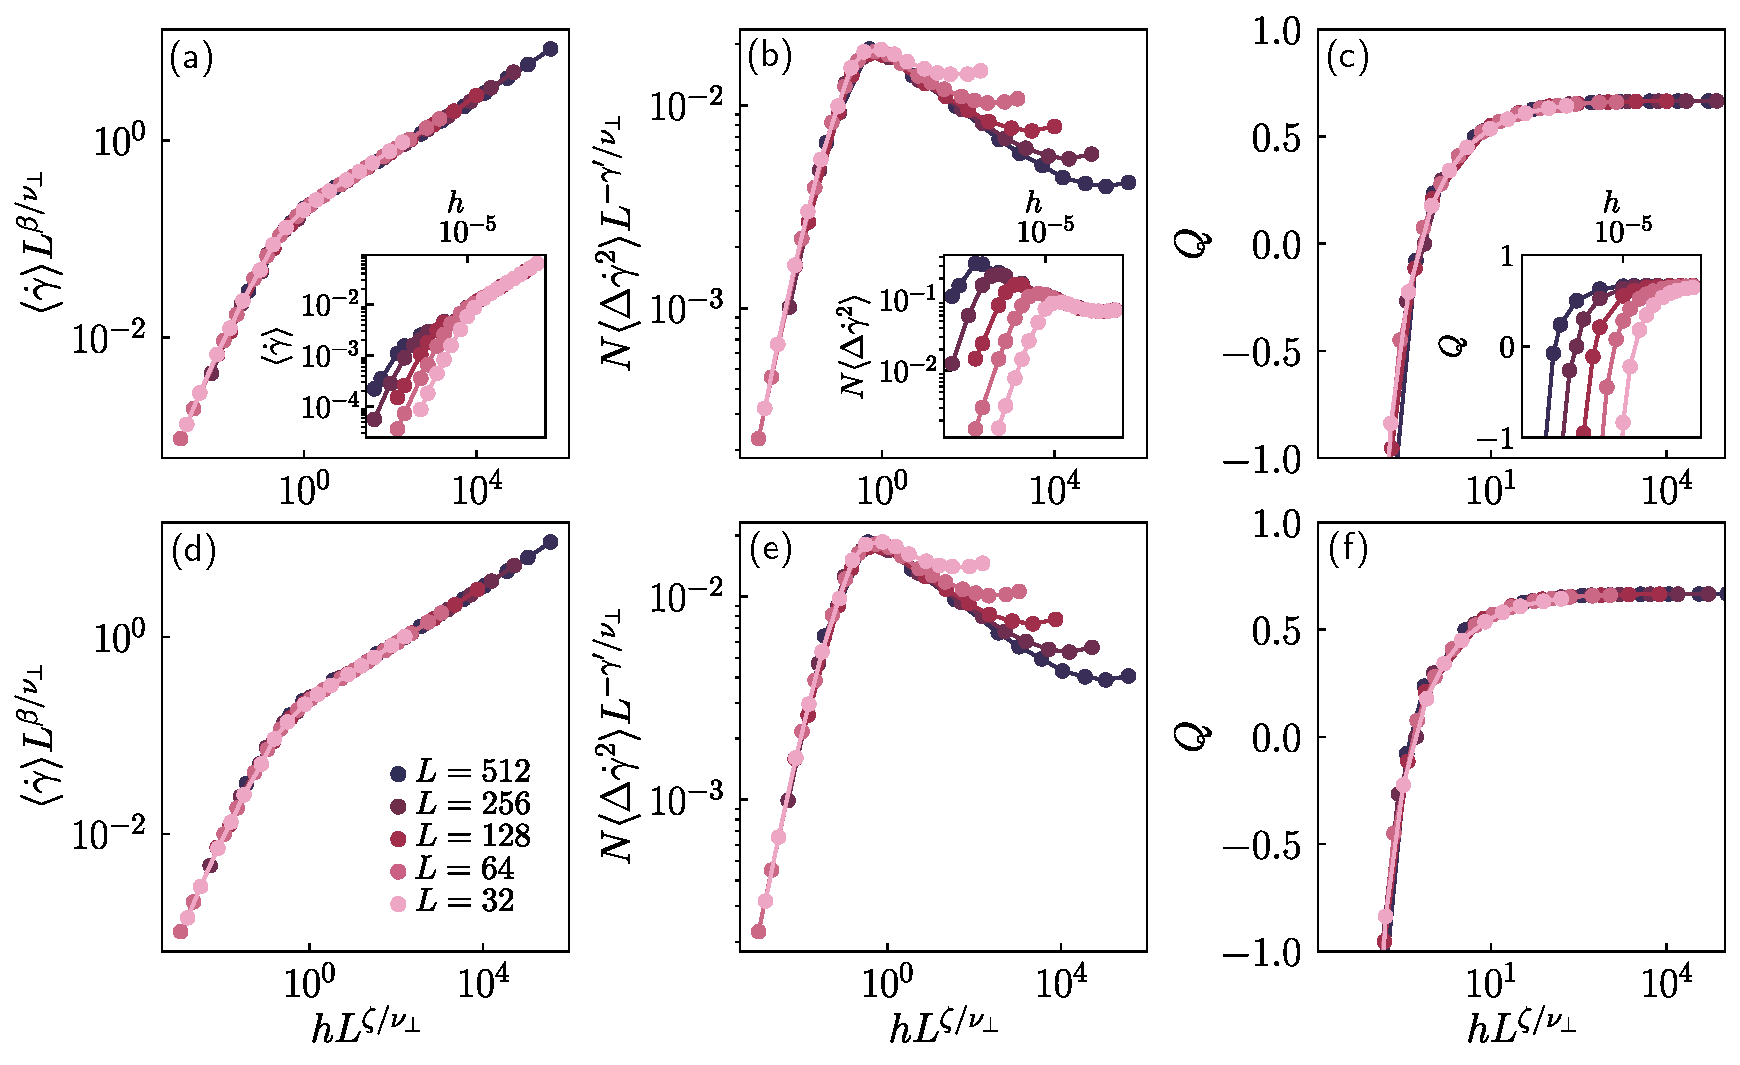
\includegraphics[width=\textwidth]{Chapitre4/Figures/CourtePortee/FSS_SRNC_edited.pdf}
	\caption{Analyse d'échelle de taille finie dans le cas du modèle $\text{FES}^\pm$. Les redimensionnements de la valeur moyenne (a), de la variance (b) et du cumulant de Binder (c) sont représentés en figures principales et les données brutes en inset. Les figures (d), (e) et (f) montrent ces mêmes redimensionnement avec les exposants connus de la classe CDP.}
	\label{fig:FSS_SRNC}
\end{figure}

\subparagraph{}Afin de confirmer que ce troisième modèle présente bien la criticalité de la percolation dirigée conservée, nous effectuons les redimensionnements des quantités avec les exposants critiques de cette classe. Les résultats sont exposés sur la \autoref{fig:FSS_SRNC}-(d)-(f). Nous observons alors que les superpositions des courbes sont aussi convaincantes dans ce cas que lors d'une estimation indépendante des exposants. Cela nous permet d'affirmer raisonnablement que ce modèle tombe donc bien dans la classe CDP. Cette analyse renforce alors l'idée que le modèle Picard-CP présente une criticalité proche mais différente du fait de sa symétrie additionnelle, le différenciant ainsi des modèles de dépiégeage à courte portée. Nous proposons alors de considérer ce nouveau comportement critique comme représentant d'une nouvelle classe d'universalité que nous appellerons CDP-0 pour des raisons évidentes.

\subparagraph{}Une critique pouvant être apposée à cette conclusion est que le modèle Picard-CP peut être sujet à des corrections d'échelle \cite{nishimori_elements_2015}. Ainsi, plus proche du point critique, pour des plus grands systèmes, la spécificité des modes zéro s'effacerait pour laisser place à la criticalité CDP. Si cette objection ne peut jamais être vraiment réfutée, la présence de telles corrections n'a pas pu être mise en évidence sur les données présentées. De plus, un autre indice penchant en faveur de notre interprétation est la visualisation de la répartition de l'activité plastique. Sur la \autoref{fig:MapsOfActSR}, nous comparons la répartition de plasticité dans le cas du modèle Picard-CP et dans le cas du modèle FES$^\pm$. Comme on peut le remarquer, il semblerait qu'à des échelles raisonnables les clusters d'activité présentent des différences. Notamment, la répartition d'activité dans le cas du modèle Picard-CP semble présenter des structures anisotropes, de compacité inférieure, suggérant un effet important des modes zéros. Il est bien sûr toujours possible qu'à plus grande échelle cette structure disparaisse, mais cet indice s'ajoute au faisceau conduisant à considérer CDP-0 comme une nouvelle classe à part entière.

\begin{figure}[h]
	\centering
	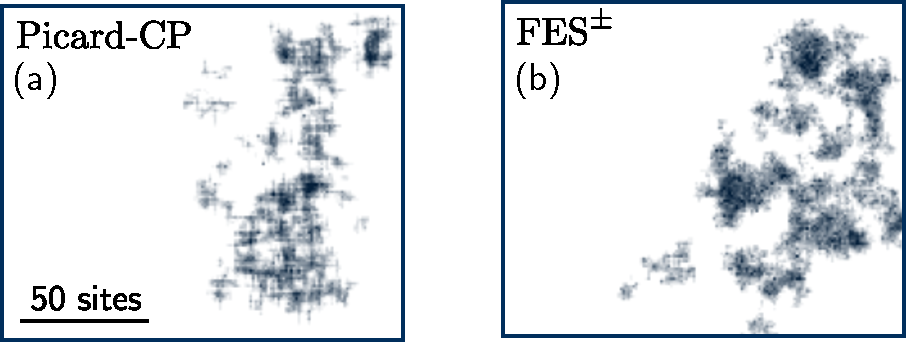
\includegraphics[width=0.65\textwidth]{Chapitre4/Figures/CourtePortee/MapsofActSR.pdf}
	\caption{Cartes d'activité plastique cumulée au cours d'une simulation pour le modèle Picard-CP (a) et le modèle $\text{FES}^\pm$ (b). Les zones foncées correspondent aux zones de forte activité plastique.}
	 \label{fig:MapsOfActSR}
\end{figure}

\paragraph{Une description continue différente}

\subparagraph{}Un dernier argument en faveur de l'existence d'une telle classe d'universalité se base sur une description en termes de théorie continue des champs. Dans le cas de la classe d'universalité CDP, la quantité conservée $\rho$ suit une dynamique non diffusive dépendante de la répartition spatiale de l'activité $A$ dans le système : $\partial_t \rho = \kappa\nabla^2 A$ (voir \autoref{chapter:introduction}). Dans notre système, le champ dynamique conservé est la contrainte $\sigma$ tandis que l'activité peut être directement associée au taux de déformation plastique $\partial_t \epsilon_{pl}$. Une description de type CDP donnerait donc :

\begin{equation}
	\partial_t \sigma(\mathbf{r},t) = \kappa\nabla^2 A(\mathbf{r},t)
\end{equation}

\noindent où l'on a noté $A(\mathbf{r},t) = \partial_t \epsilon_{pl}(\mathbf{r},t)$ pour alléger l'écriture. Cette forme d'évolution du champ de contrainte est en réalité très proche de la règle d'évolution implémentée dans les variations du modèle de Picard étudiées. On a en effet sur la grille discrète en deux dimensions :


\begin{equation}
    \partial_t\sigma_{i,j} = \sum_{k,l}G_{k,l}A_{i-k, j-l}
    \label{eq:1}
\end{equation}

\noindent où l'on a utilisé la notation discrète $f_ {ij}=f(x=ia, y=ja)$ avec $(i,j) \in \mathbb{N}^2$ et $a$ le pas du réseau. On peut alors se demander comment cette équation se traduit dans le cas continu afin d'en inférer une équation de type CDP.

\subparagraph{}Nous introduisons dans ce but les densités continues de contrainte $\sigma (x,y)$ et d'activité $A (x,y)$ associées à leurs homologues discrets  $\sigma_{i, j}$ et $A_{i, j}$:

\begin{equation}
    A_{i, j} = \left( \frac{a}{L} \right)^2A(x=i\frac{a}{L},y=j\frac{a}{L}),\quad
    \sigma_{i, j} = \left( \frac{a}{L} \right)^2\sigma(x=i\frac{a}{L},y=j\frac{a}{L})
\end{equation}

\noindent avec $L$ la taille du système. Dans la limite $(a/L) \rightarrow 0$, les densités continues correspondent aux champs de la théorie dynamique. L'équation d'évolution du modèle peut alors se ré-écrire selon :

\begin{equation}
    \partial_t\sigma (x,y) = \sum_{k,l}G_{k,l}A(x-k\frac{a}{L}, y-l\frac{a}{L}).
    \label{eq:2}
\end{equation}

\noindent Les propagateurs des deux modèles considérés étant de relative courte portée, la somme se restreint aux petites valeurs des entiers $k$ et $l$. Il est alors naturel de développer la densité continue d'activité autour de $(x,y)$ :

\begin{equation}
    A(x-k\frac{a}{L}, y-l\frac{a}{L}) = \\ \sum_{n,m=0}^{\infty}(-1)^{n+m}\left( \frac{a}{L} \right)^{n+m}\frac{k^nl^m}{n!m!}\partial_x^n\partial_y^mA(x, y)\, .
\end{equation}

\subparagraph{}De plus, dans le cas du modèle Picard-CP, le propagateur $G$ présente une symétrie $C_4$ (quadrupolaire) et des modes zéros. De ce fait, seuls les termes correspondant à des puissances $n$ et $m$ paires et strictement positives survivent à la convolution discrète. On obtient alors :

\begin{equation}
    \partial_t\sigma (x,y) = \sum_{u,v=1}^{\infty}K_{u,v}\left( \frac{a}{L} \right)^{2(u+v)}\partial_x^{2u}\partial_y^{2v}A(x, y), \quad K_{u,v} = \sum_{k,l}G_{k,l}\frac{k^{2u}l^{2v}}{(2u)!(2v)!}
\label{eq:3}
\end{equation}

\noindent Pour obtenir une description de champ de type CDP, on s'intéresse à la limite continue de grande échelle où $a/L\rightarrow 0$. Dans ce cas, le terme dominant est le premier de la somme et on a alors :

\begin{equation}
    \partial_t\sigma (x,y) = \left( \frac{a}{L} \right)^{4}K\partial_x^{2}\partial_y^{2}A(x, y), \quad K \equiv K_{1,1}
    \label{eq:evol:sigma:CDP0:raw}
\end{equation}

\noindent En redimensionnant le temps selon $t^\prime=t(a/L)^4$, nous obtenons donc finalement pour le modèle Picard-CP :

\begin{equation}
    \partial_{t^\prime}\sigma (x,y) = K\partial_x^{2}\partial_y^{2}A(x, y)\, .
    \label{eq:evol:sigma:CDP0}
\end{equation}

\subparagraph{}Dans le cas du modèle $\text{FES}^\pm$, la contrainte des modes zéros est relâchée et donc les puissances $n$ et $m$ nulles survivent aussi à la convolution, à l'exception de $(n=0,m=0)$ qui disparaît par moyenne nulle du propagateur. Dans ce cas la même procédure donne comme équation continue : 

\begin{equation}
    \partial_t\sigma (x,y) = \left( \frac{a}{L} \right)^{2}K^\prime\nabla^2 A(x, y), \quad K^\prime \equiv K_{1,0} = K_{0,1}
    \label{eq:evol:sigma:CDP:raw}
\end{equation}

\noindent Et donc en redimensionnant le temps cette fois selon $t^{\prime\prime}=t(a/L)^2$, nous obtenons :

\begin{equation}
    \partial_{t^{\prime\prime}}\sigma (x,y) = K^\prime\nabla^2 A(x, y)\, .
    \label{eq:evol:sigma:CDP}
\end{equation}

\subparagraph{}Si l'équation inférée du modèle $\text{FES}^\pm$ est bien la même que celle de la théorie CDP, celle inférée du modèle Picard-CP est fondamentalement différente. Cette différentiation orginiaire des modes zéros est remarquable, mais comprendre comment elle pourrait modifier le comportement critique associé est une tâche difficile. De plus, cela nécessiterait la détermination d'une telle équation pour le cham d'activité. Néanmoins, cela constitue un indice supplémentaire allant dans la direction de la caractérisation d'une nouvelle classe d'universalité.

\subparagraph{}L'analyse de ces deux modèles de courte portée permet donc de mettre un évidence l'importance des modes zéros et suggère donc une importance similaire dans le cas physique, en présence d'interactions à longue portée.

\subsection{Situer la transition vers l'écoulement}

\label{sec:alphaPicard}

\subparagraph{}La modification brutale de la portée dans le modèle de Picard a permis de mettre en évidence des éléments intéressants. Afin de situer ce modèle ni courte portée ni champ moyen dans une image globale compréhensible, il est nécessaire de s'intéresser au comportement critique dans le cas de portées intermédiaires. 

\subsubsection{Le modèle $\alpha$-Picard}

\subparagraph{}Pour ce faire, nous généralisons le modèle de Picard à une portée d'interaction arbitraire, i.e. $G(\mathbf{r})\sim 1/r^\alpha$. Pour conserver les propriétés centrales du propagateur classique d'Eshelby (symétrie quadrupolaire, modes zéros\footnote{implique $\hat{G}(q_x=0,q_y)=\hat{G}(q_x,q_y=0)=0$}) nous définissons cette continuité de propagateurs dans l'espace de Fourier selon :

\begin{equation}
	\hat{G}(\mathbf{q}) = -b_\alpha \frac{q_x^2 q_y^2}{q^{6-\alpha}}
\end{equation}

\noindent Dans l'espace réel, le calcul détaillé en \autoref{sec:TFinverse} donne la forme suivante pour l'interaction :

\begin{equation}
\begin{aligned}
    G(r, \theta) = B_\alpha\frac{C_\alpha+\cos 4\theta}{r^\alpha}, \quad B_\alpha &= b_\alpha\frac{\alpha\Gamma(\alpha/2-2)(\alpha-2)(\alpha-4)(2+\alpha)}{\pi 2^{9-\alpha}\Gamma(3-\alpha/2)}\\
    C_\alpha &= \frac{(\alpha-2)(4-\alpha)}{\alpha (2+\alpha)}
\end{aligned}
    \label{eq:RealAlphaPicard}
\end{equation}

\noindent avec $\Gamma$ la fonction gamma d'Euler et $b_\alpha$ étant choisi pour que $G(0)\approx-1$. Nous appelons ce modèle généralisé $\alpha$-Picard. Celui-ci coïncide alors avec le cas classique pour $\alpha=2$ ($b_2 = 4$).

\subsubsection{Implémentation numérique et instabilités}

\label{sec:instab_yielding}

\subparagraph{}En implémentant naïvement le modèle comme dans les cas précédents, les propagateurs de redistribution obtenus pour $\alpha>2$ présentent une très forte instabilité numérique (voir \autoref{fig:instabnum}-(a)). En réalité, même si moindre, cette instabilité est déjà visible dans le cas $\alpha=2$ comme c'est le cas sur la \autoref{fig:instabnum}-(b). Une méthode proposée pour remédier à cette instabilité numérique a été présentée dans \cite{nicolas_ecoulements_2014}. Celle-ci consiste à passer par un raffinement de la discrétisation. En d'autres termes, l'interaction est calculée sur une grille deux fois plus fine, puis le résultat est moyenné/coarse-grainé afin de gommer l'instabilité (qui a une période de deux sites). Cette technique fonctionne mais cache en fait un problème à la racine. 

\begin{figure}[h]
	\centering
	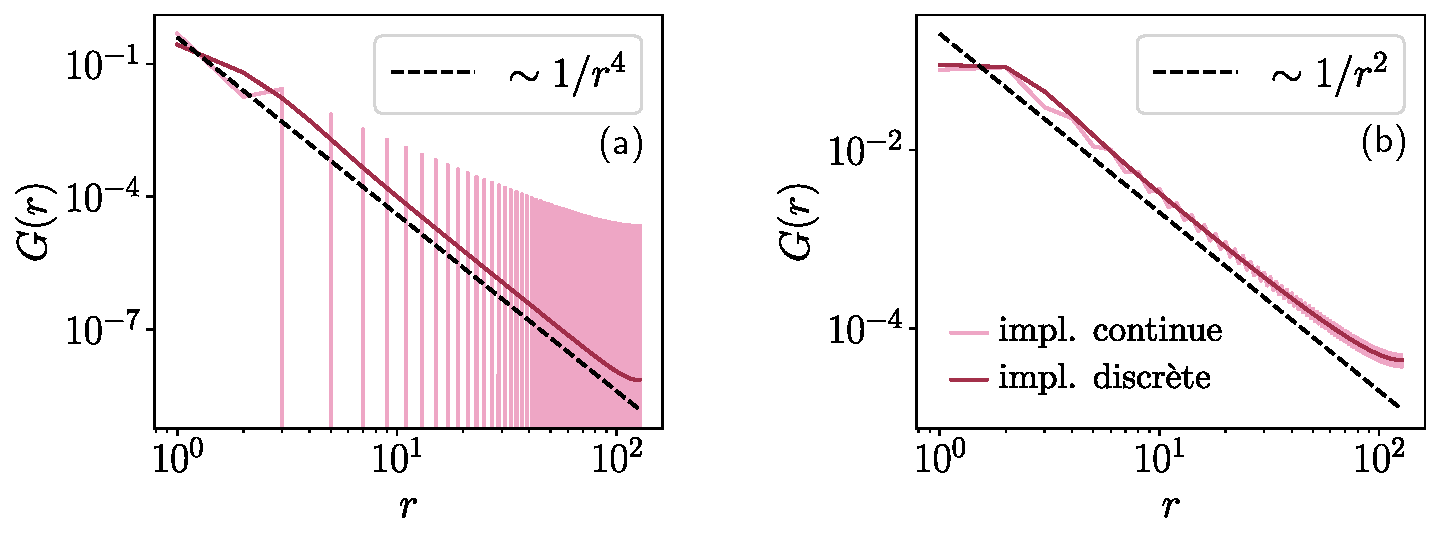
\includegraphics[width=0.85\textwidth]{Chapitre4/Figures/LonguePortee/ResolutionOscillationsPropagateur.pdf}
	\caption{Images des propagateurs de redistribution dans le modèle de Picard (a) et le modèle 4-Picard (b). Les figures montrent l'évolution du propagateur le long de la ligne $y=0$.}
	\label{fig:instabnum}
\end{figure}

\subparagraph{}L'instabilité numérique vient en réalité de l'implémentation du propagateur dans l'espace de Fourier qui est ici discret et non continu. Pour passer de la forme continue souhaitée à la forme discrète à implémenter, il faut en fait réinterpréter les nombres d'onde selon :

\begin{equation}
	q_x^2 = 2-2\cos^2\left( \frac{2\pi}{L}n \right),\quad q_y^2 = 2-2\cos^2\left( \frac{2\pi}{L}m \right)
\end{equation}

\noindent Cette méthode déjà présentée dans la littérature \cite{ferrero_criticality_2019, rossi_finite-disorder_2022} est indispensable pour obtenir des redistributions bien définies à plus courtes portées. Les corrections apportées par cette conversion sont représentées \autoref{fig:instabnum}, montrant ainsi que les instabilités peuvent être supprimées de la sorte. Les propagateurs du modèle généralisé seront donc implémentés de cette façon.

\subsubsection{Comportement critique des modèles $\alpha$-Picard}

\label{sec:criticalitealphapicard}

\subparagraph{}Nous étudions la généralisation du modèle pour $\alpha = \{1, 1.5, 3, 4, 5\}$. Pour chaque portée $\alpha$, le point critique et l'exposant $\beta$ sont déterminés à contrainte imposée. Les données et les résultats issus de ces méthodes sont consignés à la \autoref{sec:CP_aPicard}. Il est à noter que la tendance précédemment évoquée est confirmée : plus l'exposant $\beta$ mesuré est grand, plus la détermination du point critique est fastidieuse.

\subparagraph{}Sur la \autoref{fig:PLVar_EPM}-(a), nous représentons l'évolution de $\langle \dot{\gamma} \rangle$ en fonction de la distance au point critique $\delta\Sigma$ en échelle logarithmique, pour les différentes portées $\alpha$. Nous remarquons alors que plus la portée de l'interaction augmente, plus l'exposant $\beta$ augmente aussi (pente sur la représentation graphique). Par ailleurs en représentant l'évolution de la variance du taux de cisaillement, nous observons que l'on passe de fluctuations divergentes à l'approche du point critique pour les courtes portées à des fluctuations évanescentes pour les plus longues portées. Afin de mieux visualiser ces évolutions, nous traçons la courbe $\beta = f(\alpha)$ sur la \autoref{fig:PLVar_EPM}-(b). Nous remarquons alors une évolution continue de la criticalité allant de celle du modèle Picard-CP à une criticalité fortement convexe avec $\beta\approx 2$. Le cas physique $\alpha=2$ se situe alors sur cette continuité.

\begin{figure}[h]
	\centering
	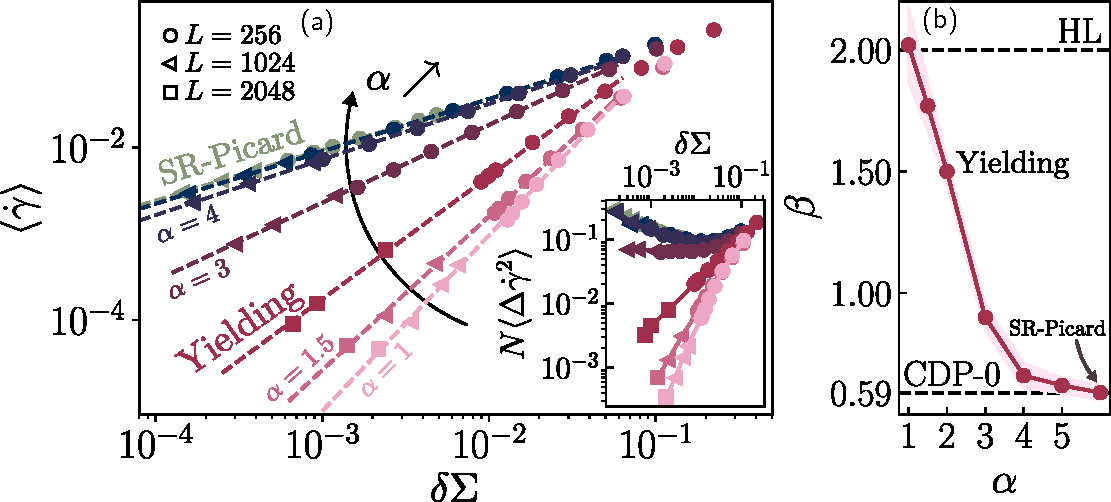
\includegraphics[width=0.9\textwidth]{Chapitre4/Figures/LonguePortee/AlphaPicard.pdf}
	\caption{(a) Courbes d'écoulement $\langle\dot{\gamma}\rangle = f(\delta\Sigma)$ pour les modèles $\alpha$-Picard $\alpha \in \{5, 4, 3, 2, 1.5, 1\}$ et pour le modèle Picard-CP.
(b) Évolution de l'exposant critique $\beta$ avec l'exposant de portée d'interaction $\alpha$.}
	\label{fig:PLVar_EPM}
\end{figure}

\subparagraph{}Plus précisément, nous observons d'abord une région entre $\alpha = 6$ et $\alpha = 4$ où l'exposant $\beta$, qui varie entre $\beta \approx 0.59$ et $\beta \approx 0.68$, dépend faiblement de la portée. Puis, entre $\alpha = 4$ et $\alpha=1$, une région où $\beta$ dépend fortement de $\alpha$ se déploie. On retrouve alors un caractère concave de la transition pour $\alpha \gtrsim 3$ et un caractère convexe pour $\alpha \lesssim 3$. Il est intéressant de noter que le point autour duquel la transition perd sa concavité semble être le même que celui pour lequel le comportement des fluctuations change ($\gamma^\prime = 0$). 

\subparagraph{}Pour les plus grandes portées le comportement critique est, comme attendu, différent de celui de la transition de dépiégeage. En effet, nous nous attendons à ce que le mécanisme défini par le bruit mécanique permette cette différence pour des exposants de bruit $\mu$ suffisamment grands et donc des portées suffisamment faibles (voir \autoref{chapter:Susp}). Toutefois pour $3<\alpha<4$, l'évolution suivie semble être sensiblement là-même que dans le cas de la transition de dépiégeage. Cela suggère donc que dans la zone $\alpha > 3$, l'influence du bruit mécanique sur la transition est secondaire. Ainsi, la compréhension de cette zone pourrait être assurée par des descriptions similaires au cadre LR-CDP.

\subsubsection{Description continue}

\subparagraph{}En suivant cette idée, nous pensons que les deux régions, d'influence faible ($4<\alpha < 6$) puis forte ($\alpha < 4$) de $\alpha$ sur $\beta$, peuvent être interprétées par un raisonnement analytique simple. Pour cela, nous allons essayer d'inférer, comme à la \autoref{sec:continuCDP0}, la bonne description continue à grande échelle de l'évolution du champ de contrainte en fonction de la portée $\alpha$. Pour ce faire, nous repartons de l'\autoref{eq:3}. Cette fois-ci, avec la forme à longue portée du propagateur que l'on notera $G^\text{LR}$, la somme dans l'expression de $K^\text{LR}_{u,v}$ ne se restreint plus uniquement aux petites valeurs de $k$ et $l$. 

\begin{equation}
	K^\text{LR}_{u,v} = \sum_{k,l}G^\text{LR}_{k,l}\frac{k^{2u}l^{2v}}{(2u)!(2v)!}
	\label{eq:sommekuv}
\end{equation}

Nous cherchons donc d'abord à évaluer $K^\text{LR}_{u,v}$ pour un propagateur décroissant comme $1/r^\alpha$. Pour ce faire, de la même manière que pour la contrainte et l'activité, nous définissons un équivalent continu du propagateur selon :

\begin{equation}
    \mathcal{G}\left(\mathbf{r}=(k\frac{a}{L},l\frac{a}{L})\right) = \left(\frac{L}{a}\right)^\alpha G_{LR}(k,l)
    \label{eq:rescaled:propagator}
\end{equation}

\noindent Dans la limite de grande échelle $a/L \rightarrow 0$, la somme peut  alors être approximée par l'intégrale de Riemann associée :

\begin{equation}
    K^\text{LR}_{u,v} = \sum_{k,l = 1}^{L/a}G_{k,l}^{LR}(k,l)k^{2u}l^{2v}
    \rightarrow \left(\frac{L}{a}\right)^{2(1+u+v)-\alpha}\int \mathrm{d}\mathbf{r}~B_\alpha\frac{C_\alpha+\cos 4\theta}{r^\alpha}x^{2u}y^{2v}
\end{equation}

\noindent et donc en intégrant :

\begin{equation}
\begin{aligned}
    K^\text{LR}_{u,v} &= \left(\frac{L}{a}\right)^{2(1+u+v)-\alpha}\int_{-\pi}^\pi \mathrm{d}\theta~B_\alpha(C_\alpha+\cos 4\theta)\cos^2\theta\sin^2\theta \int_{a/L}^1 \mathrm{d}r ~ r^{1-\alpha+2(u+v)}\\
    &=\left(\frac{L}{a}\right)^{2(1+u+v)-\alpha}\frac{\pi}{8}B_\alpha(2C_\alpha-1)\int_{a/L}^1 \mathrm{d}r ~ r^{1-\alpha+2(u+v)}\\
    &\sim \left[ \left(\frac{L}{a}\right)^{2(1+u+v)-\alpha}-1 \right]
    \label{eq:eval:I}
\end{aligned}
\end{equation}

\noindent Finalement, en ajoutant le facteur $(a/L)^{2(u+v)}$ intialement présent dans l'\autoref{eq:3}, chaque terme du développement de l'activité en $(u,v)$ se comporte comme $\left(\frac{a}{L}\right)^{\alpha-2}-\left( \frac{a}{L} \right)^{2(u+v)}$.

\subparagraph{}Pour $\alpha \geq 6$, l'évolution temporelle de la contrainte est donc dominée par le terme $(u=1,v=1)$ qui évolue comme $\left( \frac{a}{L} \right)^4$. Nous arrivons donc à une description équivalente à celle du modèle Picard-CP :

\begin{equation}
    \partial_{t^\prime}\sigma (x,y) = \tilde{K}\partial_x^{2}\partial_y^{2}A(x, y)\, .
    \label{eq:evol:sigma:Classa6}
\end{equation}

\subparagraph{}Par contre pour $\alpha < 6$, tous les termes de la somme se comportent comme $\left( \frac{a}{L} \right)^{\alpha-2}$. Aucun ordre dominant du développement ne se détache et l'on doit donc considérer la somme dans son ensemble. L'évolution temporelle de la contrainte à grande échelle doit donc faire intervenir la convolution complète dans la limite continue.

%\subparagraph{}Pour traiter ce cas et aller un peu plus loin, nous repartons de l'équation générale (\autoref{eq:2}). En utilisant les propriétés de symétrie du propagateur, nous pouvons ré-écrire astucieusement :
%
%\begin{equation}
%\begin{aligned}
%    \partial_t\sigma (x,y) =& \sum_{k,l}G_ {k,l}\Big(A(x-k\frac{a}{L}, y-l\frac{a}{L})-A(x,y)\\
%    &-\left(k\frac{a}{L}\right)^2\partial_x^2A(x,y)-\left(l\frac{a}{L}\right)^2\partial_y^2A(x,y)
%    -kl\frac{a}{L}\partial_x\partial_yA(x,y)\Big)
%\end{aligned}
%\end{equation}
%
%\noindent puisqu'aucun des termes ajoutés ne survit à la convolution. Ceci est dû à la symétrie $C_4$ et à la propriété de modes zéros du propagateur. En prenant la limite continue de grande échelle comme précédemment, on obtient alors :
%
%\begin{equation}
%   \partial_t \sigma(\mathbf{r}) = \left( \frac{a}{L} \right)^{\alpha - 2}\int_{\theta=-\pi}^\pi\int_{r=a/L}^{1} \mathrm{d}\mathbf{r}^\prime ~ \mathcal{G}(\mathbf{r}^\prime)
%     \times\left( A(\mathbf{r}-\mathbf{r}^\prime)-A(\mathbf{r})-\frac{1}{2}r_i^\prime r_j^\prime \partial_i\partial_jA(\mathbf{r}) \right)
%    \label{eq:evol:sigma:LR:raw}
%\end{equation}
%
%\noindent Le propagateur de redistribution tombant comme $\mathcal{G}(\mathbf{r})\propto r^{-\alpha}$ et étant donné qu'à petits $\mathbf{r}^\prime$ on a :
%
%\begin{equation}
%A(\mathbf{r}-\mathbf{r}^\prime)-A(\mathbf{r})-\frac{1}{2}r_i^\prime r_j^\prime \partial_i\partial_jA(\mathbf{r}) \sim\mathcal{O}(r^{\prime 4}),
%\end{equation}
%
%\noindent l'intégrale sur $r'$ de l'équation \autoref{eq:evol:sigma:LR:raw} converge à sa borne inférieure seulement si $\alpha < 6$. Dans ce cas l'évolution temporelle de la contrainte se comporte comme $\left( \frac{a}{L} \right)^{\alpha - 2}$. Cependant pour $\alpha>6$, l'intégrale diverge et la description perd sa validité. Dans ce cas, le comportement à grande échelle est celui déterminé précédemment et décrit par l'\autoref{eq:evol:sigma:Classa6}.

\paragraph{Comparaison avec la transition de dépiégeage}

\subparagraph{}Pour comprendre l'influence des modes zéros sur cette description, nous pouvons mener la même étude sur un propagateur de type dépiégeage à longue portée, i.e. isotrope, sans modes zéros. Sans ces derniers, la description comme interaction de courte portée est celle du modèle $\text{FES}^\pm$ présentée \autoref{eq:evol:sigma:CDP}. La somme de l'\autoref{eq:sommekuv} est alors dominée par un terme de courte portée se comportant comme $\left(  \frac{a}{L}\right)^2$ pour $\alpha>4$ cette fois. Dans ce cas, la description adéquate est celle de CDP.

\subparagraph{}Pour le cas $\alpha<4$, la convolution complète doit être considérée car aucun terme du développement ne domine le comportement d'échelle. Dans ce cas, l'évolution temporelle de la contrainte se comporte alors comme $\left(  \frac{a}{L}\right)^{\alpha-2}$, exactement de la même manière qu'avec la présence de modes zéros.

%On a alors :
%
%\begin{equation}
%    \left( \frac{a}{L} \right)^{\alpha - 2}\int_{\theta=-\pi}^\pi\int_{r=a/L}^{1} \mathrm{d}\mathbf{r}^\prime ~ \mathcal{G}(\mathbf{r}^\prime)
%    \left( A(\mathbf{r}-\mathbf{r}^\prime)-A(\mathbf{r})\right)
%\end{equation}
%
%\noindent qui converge bien uniquement pour $\alpha<4$ puisque le terme $\frac{1}{2}r_i^\prime r_j^\prime \partial_i\partial_jA(\mathbf{r})$ ne peut plus être ajouté librement cette fois dans la convolution. 

\paragraph{Raisonnement simple dans l'espace réciproque}

\subparagraph{}Ces résultats peuvent être tout aussi bien déduits d'une analyse d'échelle simple dans l'espace réciproque. Dans le cas de la transition vers l'écoulement, nous avons montré que le terme d'interaction de courte portée avait la forme donnée par l'\autoref{eq:evol:sigma:Classa6}. Dans l'espace réciproque il est donc représenté par un terme en $\sim q^4$. L'interaction à longue portée, elle, se comporte comme $\frac{q_x^2q_y^2}{q^{6-\alpha}}$, soit en $\sim q^{\alpha-2}$. Ainsi, selon le raisonnement déjà présenté dans le cadre LR-CDP au \autoref{chapter:TransportLP}, nous nous attendons à ce que le terme de longue portée domine pour $\alpha < 6$ et que le terme de courte portée domine pour $\alpha > 6$.

\subparagraph{}Dans le cadre de la transition de dépiégeage, l'interaction de courte portée se comporte comme $\sim q^2$ dans l'espace réciproque alors que l'interaction de longue portée, représentée par l'opérateur fractionnaire $-|\nabla|^{\alpha-D}$ se comporte comme $q^{\alpha-2}$. Dans ce cas, nous nous attendons à ce que le terme de longue portée domine pour $\alpha < 4$ et que le terme de courte portée domine pour $\alpha > 4$.

\subparagraph{}Ainsi, la présence de modes 0 dans les interactions ouvre une zone d'influence des interactions à longue portée située en $\alpha = 6$ et $\alpha = 4$.

\subsubsection{Paysage global}

\subparagraph{}Ces comportements d'échelle suggèrent donc un paysage en trois régions distinctes :

\begin{itemize}
	\item Une première région pour $\alpha>6$ dont la criticalité est dominée par les interactions à courte portée. La classe supposée décrire ce comportement est alors CDP-0, représentée par le modèle Picard-CP.
	\item Une seconde région $4<\alpha<6$ où les interactions à longue portée démarrent leur influence sur le comportement critique. Cette région est spécifique à la présence de modes zéros. Nous la nommons $\text{LP-0}$.
	\item Une troisème région $\alpha <4$ où la portée de l'interaction maintient son influence sur le comportement critique mais dont la spécificité ne tient plus aux modes zéros. L'analyse d'échelle ne permet en effet pas de la différencier de la région homologue associée au dépiégeage à longue portée.
\end{itemize}

\subparagraph{}Ce court raisonnement analytique nous permet donc de confirmer la tendance observée numériquement pour l'identification de la région LP-0, où le comportement critique dépend a priori uniquement légèrement de la portée. Toutefois, celui-ci ne permet pas de faire la différence entre une interaction de type dépiégeage et les interactions avec modes zéros du modèle $\alpha$-Picard pour $\alpha<4$. \`A la place, nous pensons que cette différenciation que l'on remarque effectivement sur l'évolution de l'exposant $\beta$, plus spécifiquement pour $\alpha = 3$, est principalement due à la présence d'un bruit mécanique dans le cas de la transition vers l'écoulement. Nous nommons cette zone $\text{LP}$.

\subparagraph{}Dans le cas du dépiégeage, la zone de longue portée (nommée Dep-LP sur la \autoref{fig:YieldingLandscape}) où les exposants dépendent continûment de $\alpha$ est située entre $\alpha=4$ et $\alpha=3$. Ce comportement entre dans le cadre de référence LR-CDP. Pour $\alpha<3$, le comportement critique devient celui du champ moyen avec $\beta=1$.

\subparagraph{}Pour la transition vers l'écoulement, la zone $3<\alpha<4$ montre une évolution similaire en fonction de $\alpha$ avec $\beta$ allant de $\beta\approx 0.68$ à $\beta\approx 0.95$. Pour être conclusif quant à l'équivalence avec le dépiégeage dans cette région, il faudrait étendre notre étude à des portées intermédiaires. Pour $\alpha<3$ cependant, le comportement critique ne semble pas avoir atteint celui du champ moyen puisque $\beta$ continue d'augmenter jusqu'à $\alpha=1$, pour lequel on mesure $\beta\approx 2$. Par ailleurs, le modèle de Hébraud-Lequeux, préssenti pour représenter les modèles élastoplastiques en champ moyen, montre une criticalité de type $\beta=2$. Par analogie avec les comportements de longue portée canoniques, nous suggérons alors que pour $\alpha<1$, le système admet un comportement champ moyen (nommé CM sur la \autoref{fig:YieldingLandscape}). Cette conjecture pour la limite de champ moyen est partagée par l'étude de Lin et. al \cite{lin_mean-field_2016} dont nous discuterons au chapitre suivant.

\begin{figure}[h]
	\centering
	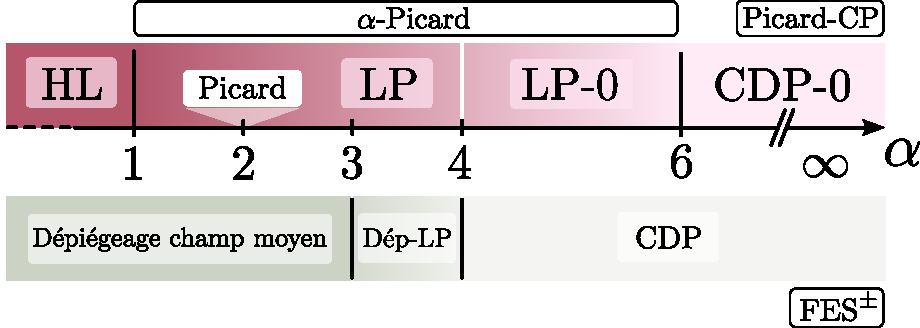
\includegraphics[width=0.7\textwidth]{Chapitre4/Figures/LonguePortee/axe_alpha.pdf}
	\caption{Axe supérieur : classification du comportement à grande échelle des modèles d'écoulement en fonction de l'exposant de portée $\alpha$. Axe inférieur : représentation équivalente pour les modèles de dépiégeage \cite{cao_localization_2018}.}
	\label{fig:YieldingLandscape}
\end{figure}

\subparagraph{}In fine, les élements que nous apportons suggèrent de placer la criticalité des modèles $\alpha$-Picard sur un paysage décrit à la \autoref{fig:YieldingLandscape}. La transition vers l'écoulement, représentée par le modèle de Picard, se situe donc dans une région de longue portée où le comportement critique dépend encore continûment de l'exposant $\alpha$. Cette localisation dans une image globale nous permet de mettre en évidence des ingrédients qui jouent un rôle clé dans le phénomène, notamment la présence de modes zéro. Enfin, la comparaison avec le dépiégeage dont on rapproche souvent cette transition, montre des évolutions profondément différentes. En effet, la zone de longue portée dans le cas de la transition vers l'écoulement est bien plus large ($1<\alpha<6$) que dans le cas du dépiégeage ($3<\alpha<4$) et la description équivalente à courte portée semble être issue d'une classe d'universalité différente. Si un point ressemblant au champ moyen du dépiégeage semble pouvoir être atteint autour de $\alpha\approx 3$, le mécanisme de bruit interne dans la transition vers l'écoulement semble permettre de le dépasser pour faire apparaître un autre champ moyen de type Hébraud-Lequeux.

\subparagraph{}Il est alors intéressant de voir si les autres propriétés critiques du système suivent cette même évolution caractéristique.

\subsection{Influence de la portée sur les corrélations de contrainte dans l'état stationnaire}

\subparagraph{}Si notre étude statique s'est essentiellement concentrée sur des propriétés très globales du système, nous proposons dans cette partie de nous intéresser à une observable plus structurelle. Plus particulièrement, une propriété intéressante des systèmes appartenant à la classe CDP est celle d'hyperuniformité, définie au \autoref{chapter:introduction}.

\subsubsection{Hyperuniformité dans les modèles élastoplastiques}

\subparagraph{}Dans les modèles de particules appartenant à la classe CDP, l'hyperuniformité se traduit par une évanescence du facteur de structure $S(\mathbf{q})$ à petits nombres d'onde :

\begin{equation}
	S(\mathbf{q})\sim q^{\alpha_\text{HU}}, \quad 0<\alpha_\text{HU}<1
\end{equation}

\noindent Dans une théorie continue, le facteur de structure est défini via la transformée de Fourier $\hat{\rho}(\mathbf{q})$ de la densité particulaire $\rho(\mathbf{r})$ selon :

\begin{equation}
	S(\mathbf{q}) \propto  \langle \hat{\rho}(\mathbf{q})\hat{\rho}(\mathbf{-q}) \rangle
\end{equation}

\noindent $\langle \cdot \rangle$ désignant une moyenne sur les réalisations du système.

\subparagraph{}Dans le cadre de la transition vers l'écoulement via l'approche élastoplastique, la notion de particules est absente. Il n'est donc pas évident de voir comment cette propriété pourrait se reporter dans ce cas. Une première approche naïve correspond alors à l'analogie opérée lors de l'établissement des équations continues \autoref{sec:continuCDP0}. Dans les modèles élastoplastiques, le champ conservé est le champ de contrainte. Dans les modèles de particules, le champ conservé est la densité de particules. Dans les modèles élastoplastiques, l'activité induit une redistribution de la contrainte : le site actif relaxe sa contrainte et, en moyenne, en ajoute aux autres sites. Dans les modèles de particules, l'activité induit une redistribution de la masse : un site actif perd des particules qui viennent s'ajouter aux autres sites.

\subparagraph{}Il est alors naturel de penser que la contrainte $\sigma$ dans le cas des modèles élastoplastiques joue le même rôle que la densité $\rho$ dans les modèles de particules. Dans ce cas, nous pouvons supposer que pour un modèle élastoplastique tombant dans la classe CDP comme le modèle $\text{FES}^\pm$, nous obtiendrions :

\begin{equation}
	S_\sigma(\mathbf{q}) \equiv \langle\hat{\sigma}(\mathbf{q})\hat{\sigma}(\mathbf{-q})\rangle \sim q^{\alpha_\text{HU}^\text{CDP}}
\end{equation}

\noindent $S_\sigma(\mathbf{q})$ n'étant alors rien d'autre que la transformée de Fourier de la fonction de corrélation connectée de contrainte :

\begin{equation}
	C_{\sigma\sigma}(\mathbf{r}) = \langle \sigma(\mathbf{r^\prime})\sigma(\mathbf{\mathbf{r}^\prime-\mathbf{r}})\rangle_c
\end{equation}

\noindent qui est un objet d'étude bien plus étudié par la communauté des fluides à seuil \cite{chowdhury_long_2016, maier_emergence_2017, lerner_simple_2020}.

\subparagraph{}On peut alors se demander si ce comportement évanescent de $S_\sigma(\mathbf{q})$ à petits nombres d'onde se retrouve aussi dans les modèles élastoplastiques étudiés précédemment.

%\subsubsection{Approche naïve et hydrodynamique fluctuante}
%
%\subparagraph{}Un raisonnement analytique simple permet de conforter l'intuition que les corrélations de contrainte suivent un comportement sans échelle proche de la transition. Celui-ci repose sur le calcul de la fonction $S_\sigma(\mathbf{q})$ en interprétant la dynamique du système dans le cadre de l'hydrodynamique fluctuante \cite{chaikin_principles_1995}. 
%
%\subparagraph{}Pour ce faire, nous considérons les équations de champ CDP modifiées selon :
%
%\begin{equation}
%    \begin{aligned}
%        \partial_t\sigma(\mathbf{r}, t) &= \left(\mathcal{G}\ast A \right)(\mathbf{r}, t)\\
%        \partial_t A(\mathbf{r}, t) &= (\kappa\sigma(\mathbf{r}, t)-\varsigma)A(\mathbf{r}, t)-\lambda A^2(\mathbf{r}, t) + D_A\Delta A(\mathbf{r}, t)
%        +\chi \sqrt{A(\mathbf{r}, t)}\eta
%    \end{aligned}
%\end{equation}
%
%\noindent comme une première possible approximation de la théorie de champ associée à ces modèles. Suivant les méthodes classiques d'hydrodynamique fluctuante, nous linéarisons ces équations en décomposant les champs comme $A(\bm{r}, t) = A_0 +\delta A(\bm{r}, t)$ et $\sigma(\bm{r}, t) = \sigma_0 +\delta \sigma(\bm{r}, t)$ avec $\langle\delta A(\bm{r}, t)\rangle = \langle \delta \sigma(\bm{r}, t)\rangle = 0 $. Après transformées de Fourier spatiale et temporelle des équations, nous obtenons :
%
%\begin{equation}
%    \langle\delta\hat{\sigma}(\bm{q}, \omega)\delta\hat{\sigma}(\bm{q}', \omega')\rangle = \frac{\chi^2 A_0 \hat{\mathcal{G}}(\bm{q})^2 \delta(\omega+\omega')\delta(\bm{q} + \bm{q}')}{|\omega^2 + i\omega (\lambda A_0 + D_A q^2) + \kappa A_0 \hat{\mathcal{G}}(\bm{q})|^2}\, .
%\end{equation}
%
%\noindent Nous intégrons ensuite sur les fréquences $\omega$ en utilisant le théorème des résidus pour obtenir :
%
%\begin{equation}
%    S_{\sigma}(\mathbf{q}) = -\frac{\chi^2\hat{\mathcal{G}}(\bm{q})}{2\kappa(\lambda A_0 + D_A q^2)}
%\end{equation}
%
%\subparagraph{}Dans la limite de grande échelle $q\rightarrow 0$, on attend donc :
%
%\begin{equation}
%    S_{\sigma}(\mathbf{q}) \sim -\hat{\mathcal{G}}(\bm{q})
%\end{equation}
%
%\noindent si bien que les corrélations de contrainte sont à l'image du propagateur de redistribution. Ce comportement sur la répartition de contrainte est par ailleurs connu pour les fluides à seuil au repos \cite{lerner_simple_2020}, où elle prend la forme du propagateur de Eshelby. Dans le cas du modèle $\alpha$-Picard, ce raisonnement simple suggère bien une propriété hyperuniforme à courte portée avec $\hat{\mathcal{G}}(\bm{q})\sim q^4$ dans le modèle Picard-CP, propriété probablement perdue dans le cas physique où l'on a $\hat{\mathcal{G}}(\bm{q})\sim q^0$ (voir \autoref{eq:eshelbydiscretfourier}).

\subsubsection{Approche par le dépiégeage}

\subparagraph{}En fait, une approche plus rigoureuse permet de pressentir une forme d'hyperuniformité sur la contrainte. Celle-ci se base sur la ressemblance entre les modèles de type dépiégeage et les modèles élastoplastiques. Dans le cas du dépiégeage, il n'y a pas non plus de quantité physiquement évidente pour laquelle on pourrait supposer une propriété d'hyperuniformité. Toutefois, comme nous l'avons mentionné au \autoref{sec:introduction}, celle-ci est en lien direct avec les propriétés de rugosité de l'interface.

\subparagraph{}En fournissant une compréhension plus simple de l'équivalence entre les deux phénomènes critiques, K. Wiese \cite{wiese_hyperuniformity_2024} a en effet pu faire un parallèle direct entre la densité $\rho$ dans les modèles de particules et la position de l'interface $u$ dans les modèles de dépiégeage, qui est :

\begin{equation}
	\rho(\mathbf{r},t) \sim \Delta u(\mathbf{r},t) + \rho_0
\end{equation}

\noindent dans le cas de courte portée, avec $\rho_0$ la densité moyenne de particules. Le terme $\Delta u(\mathbf{r},t)$ ne représente alors rien d'autre que l'interaction élastique entre les différents points du système. Ainsi, l'équivalent du déplacement dans nos simulations élastoplastiques étant la déformation plastique $
\epsilon_{pl}(\mathbf{r},t)$, la quantité équivalente à $\rho$ dans ce cas serait :

\begin{equation}
	\rho (\mathbf{r},t) \sim \left(\mathcal{G}\ast\epsilon_{pl}\right)(\mathbf{r},t)+ \rho_0
\end{equation}

\noindent Donc d'après l'\autoref{eq:DynPicardInteg} de la dynamique intégrée on aurait :

\begin{equation}
	\rho (\mathbf{r},t) - \rho_0 \sim \sigma (\mathbf{r},t)- \Sigma
\end{equation}

\noindent ce qui confirme l'intuition initiale.

\subparagraph{}De cette équivalence, le travail \cite{wiese_hyperuniformity_2024} parvient à relier l'exposant d'hyperuniformité $\alpha_\text{HU}$ du modèle Manna à l'exposant de rugosité $\eta$ du dépiégeage avec la relation d'échelle :

\begin{equation}
	\alpha_\text{HU} = 4 - D - 2\eta
\end{equation}

\noindent que l'on peut généraliser dans notre cas pour une portée arbitraire $\alpha$ du propagateur :

\begin{equation}
	\alpha_\text{HU} = 2\alpha - 3D - 2\eta
	\label{eq:scalingHULP}
\end{equation}

\noindent Le cas des modèles élastoplastiques est alors très intéressant puisque ceux-ci constituent des modèles dans lequel les deux exposants à la fois ont un sens physique intéressant. L'exposant $\alpha_\text{HU}$ qualifie la répartition de la contrainte et l'exposant $\eta$ la répartition des zones de plasticité accumulée au cours du temps. (\rem{reformuler ?})

\subsubsection{Résultats numériques}

\label{sec:HUEPM}

\paragraph{Méthode}

\subparagraph{}Afin de sonder les propriétés de répartition de contrainte dans les modèles étudiés, nous nous plaçons, pour chaque modèle, dans un état stationnaire du système proche du point critique ($\delta\Sigma \ll 1$). La fonction $S_\sigma(\mathbf{q})$ est alors calculée en tout point de l'espace réciproque en prenant la transformée de Fourier du champ de contrainte discret $\{\sigma_i\}$ après lui avoir soustrait sa valeur moyenne $\Sigma$. 

\subparagraph{}Afin d'obtenir une estimation propre de ce pseudo-facteur de structure et ce sur une large gamme de $\mathbf{q}$, il est nécessaire de ne pas limiter le calcul à une unique configuration. Pour ce faire, nous réalisons pour une même mesure une centaine de simulations issues de conditions initiales différentes. La mesure finale est alors la moyenne de chaque mesure individuelle. Afin de sonder des valeurs de $\mathbf{q}$ suffisamment petites, nous choisissons de nous placer à une taille de système suffisamment grande, ici $L=1024$.

\paragraph{Confirmation de l'analogie via le modèle $\text{FES}^\pm$}

\subparagraph{}Nous appliquons tout d'abord cette méthode de mesure au cas du modèle $\text{FES}^\pm$, duquel on attend une criticalité de type CDP, et donc celle du dépiégeage. Pour ce faire, nous nous plaçons à une distance $\delta\Sigma = 1.5\times 10^{-4}$ du point critique. Celle-ci constitue la plus petite distance permettant d'atteindre l'état stationnaire en une itération de simulation.

\subparagraph{}Les résultats obtenus sont alors présentés à la \autoref{fig:SfactStressFES}-(a). La carte des valeurs du pseudo-facteur de structure indique bien une diminution à petits nombres d'onde. Sa structure est par ailleurs légèrement anisotrope, ceci étant probablement dû aux conditions périodiques appliquées\footnote{Il est à noter que cette représentation est linéaire en $q$. Dans la zone de petits $q$ qui nous intéresse, la fonction est globalement isotrope}. Afin de quantifier plus précisément cette propriété, nous regardons l'évolution de $S_\sigma(\mathbf{q})$ sur la ligne $q_x = 0$. L'évolution obtenue est alors représentée sur la \autoref{fig:SfactStressFES}-(b).

\begin{figure}[h]
	\centering	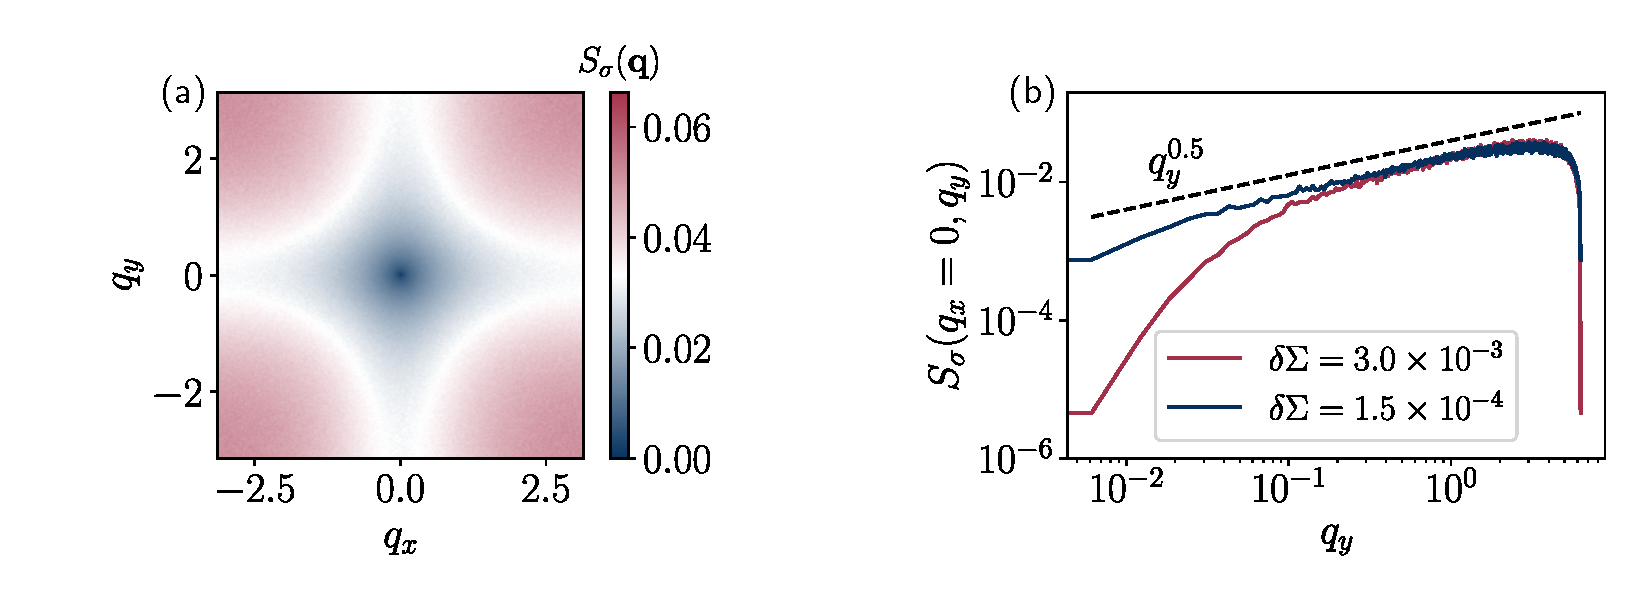
\includegraphics[width=\textwidth]{Chapitre4/Figures/Correlations/Sfact_SRPNC.pdf}
	\caption{Évolution du pseudo-facteur de structure dans le modèle $\text{FES}^\pm$. (a) carte de valeurs du pseudo-facteur de structure $S_\sigma(\mathbf{q})$ dans l'espace réciproque discret. (b) Évolution du pseudo-facteur de structure le long de la ligne $q_x=0$.}
	\label{fig:SfactStressFES}
\end{figure}

\subparagraph{}Nous observons alors effectivement une évanescence en loi de puissance à petits $q_y$, qui semble parfaitement compatible avec l'exposant d'hyperuniformité associé à la classe CDP, $\alpha_\text{HU}^\text{CDP} = 0.5$. En effectuant la même mesure légèrement plus loin du point critique pour $\delta\Sigma = 3.0\times 10^{-3}$, un comportement similaire est observé, seulement sur une plage plus restreinte de nombres d'onde. Cela suggère donc qu'au point critique on a bien $S_\sigma(\mathbf{q})\sim q^{0.5}$ pour tout $q\ll 1$, confirmant ainsi les parallèles entre densité et contrainte présentés précédemment.

\begin{figure}[h]
	\centering	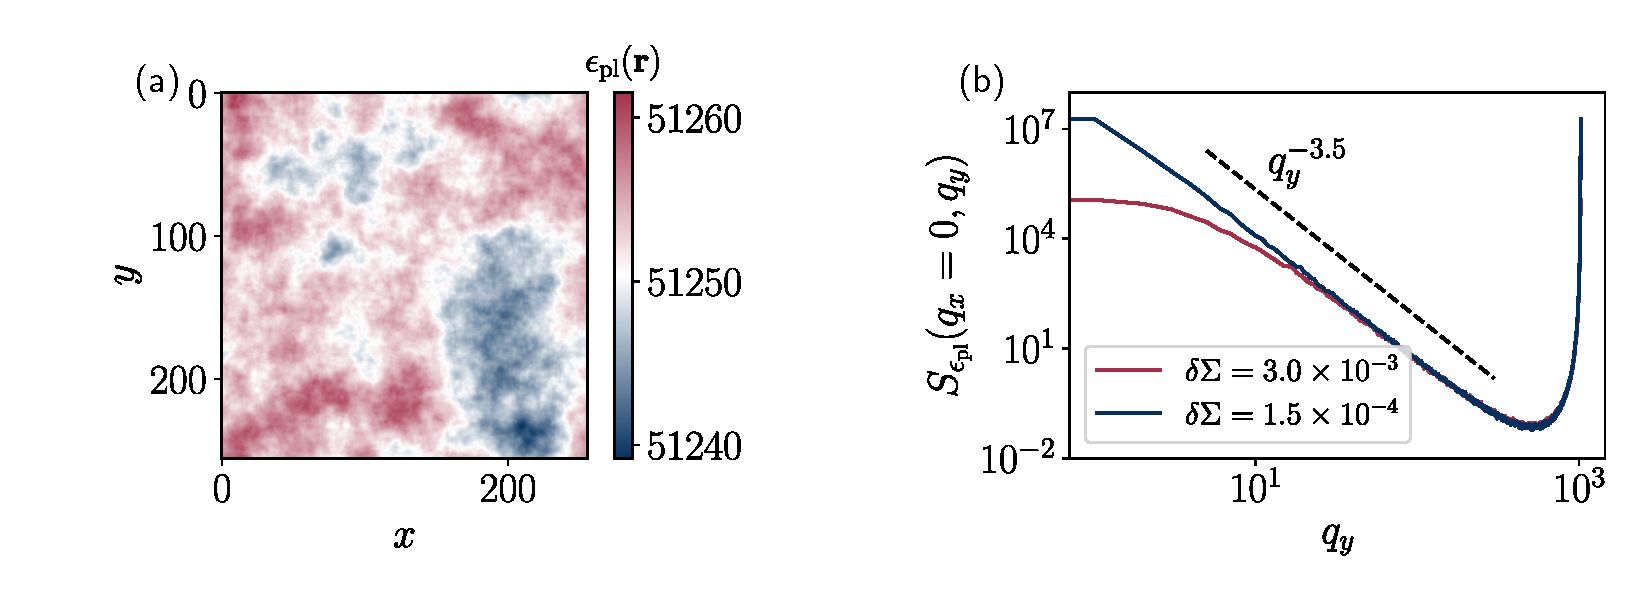
\includegraphics[width=\textwidth]{Chapitre4/Figures/Correlations/Sfact_Disp_SRPNC.pdf}
	\caption{(a) Répartition spatiale du déplacement plastique $\epsilon_\text{pl}(\mathbf{r})$ dans le modèle $\text{FES}^\pm$ pour une simulations avec $\delta\Sigma = 1.5\times 10^{-4}$. (b) Évolution du spectre du déplacement plastique $S_{\epsilon_\text{pl}}(\mathbf{q})$ le long de la ligne $q_x=0$.}
	\label{fig:SfactDispFES}
\end{figure}

\subparagraph{}Nous pouvons par ailleurs mesurer les corrélations de déplacement dans le matériau afin d'évaluer la rugosité de l'interface. En effet, si l'on note de la même manière $S_{\epsilon_\text{pl}}(\mathbf{q})$ le spectre du déplacement plastique on a alors :

\begin{equation}
	S_{\epsilon_\text{pl}}(\mathbf{q}) \sim q^{-D-2\eta}
\end{equation}

\noindent par définition de l'exposant de rugosité. En appliquant la même méthode que précédemment, nous obtenons les résultats présentés à la \autoref{fig:SfactDispFES}. Nous mesurons alors $D+2\eta \approx 3.5$ soit $\eta\approx 0.75$, qui est bien la valeur attendue dans le cas du dépiégeage à courte portée en deux dimensions \cite{semeikin_roughness_2024}. Ces mesures de structure semblent donc confirmer l'appartenance du modèle $\text{FES}^\pm$ à la classe CDP. Notons par ailleurs que ces mesures d'hyperuniformité sont bien plus évidentes que dans le cas des modèles de particules, dans le sens où nous observons ici des lois de puissance claires. Ceci peut potentiellement s'expliquer par le fait d'une redistribution continue et non discrète dans le cas des modèles élastoplastiques.

\paragraph{Hyperuniformité dans le modèle $\alpha$-Picard}

\subparagraph{}Pour comprendre comment cette propriété d'hyperuniformité se compare dans le cas des modèles d'écoulement, nous effectuons la même analyse sur les généralisations du modèle de Picard. Dans le cas du modèle Picard-CP, les résultats obtenus sont présentés à la \autoref{fig:SfactStressPCP}.

\begin{figure}[h]
	\centering
	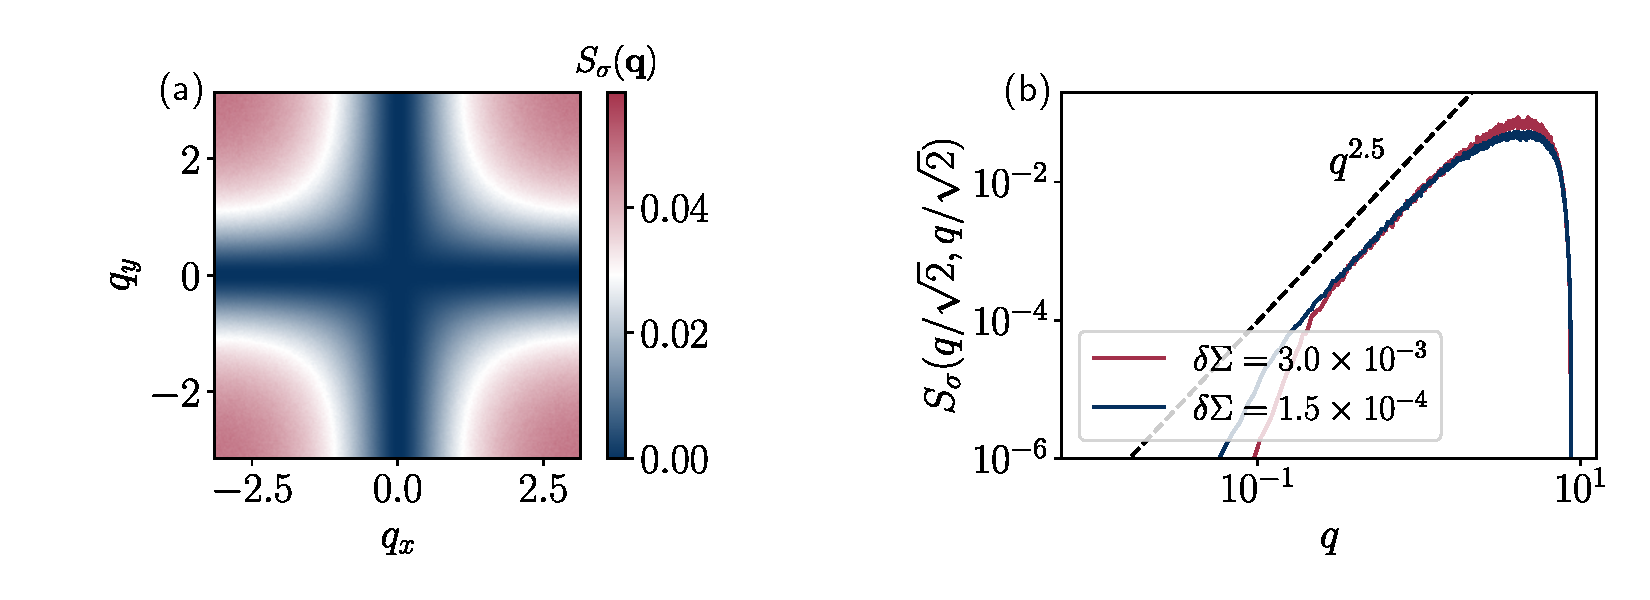
\includegraphics[width=\textwidth]{Chapitre4/Figures/Correlations/Sfact_SRP.pdf}
	\caption{Évolution du pseudo-facteur de structure dans le modèle Picard-CP. (a) carte de valeurs du pseudo-facteur de structure dans l'espace réciproque discret. (b) Évolution du pseudo-facteur de structure le long de la diagonale $(q_x=\frac{q}{\sqrt{2}},q_y=\frac{q}{\sqrt{2}})$.}
	\label{fig:SfactStressPCP}
\end{figure}

\subparagraph{}La carte de valeurs de $S_\sigma(\mathbf{q})$ montre alors une anisotropie frappante dont les axes de symétrie sont ceux associés aux modes zéros ($q_x=0$ et $q_y=0$). Le pseudo-facteur de structure prend alors des valeurs proches de 0 sur ces axes. Cette propriété d'anisotropie découle en fait trivialement de l'\autoref{eq:DynPicardInteg} car dans l'espace de Fourier le champ de contrainte est une multiplication du propagateur et du champ de déplacement. Il semble donc compliqué de réduire cette analyse à un problème monodimensionnel, i.e. en regardant l'évolution de $S_\sigma(\mathbf{q})$ sur une ligne, puisque chaque choix de direction produira vraisemblablement une évolution différente.

\subparagraph{}Afin de pouvoir pousser l'analyse tout de même plus loin, nous choisissons de nous intéresser à la direction définie par la bissectrice de ces axes et donc de considérer la diagonale $(q_x = q/\sqrt{2}, q_y = q/\sqrt{2})$. L'évolution le long de cette ligne est représentée \autoref{fig:SfactStressPCP}-(b). Nous observons alors toujours une évanescence de $S_\sigma(\mathbf{q})$ mais cette fois-ci bien plus abrupte avec $\alpha_\text{HU} \approx 2.5$. Cette mesure constitue alors un nouvel indice rejoignant la ligne qui suggère de séparer les comportements critiques du modèle Picard-CP et de la classe CDP.

\subparagraph{}Si l'hyperuniformité semble être fortement affectée par les modes zéros à courte portée, il nous semble intéressant d'observer comment la longue portée, elle, joue un rôle dans cette structure de contraintes. Notamment, si dans le cas classique ces corrélations suivent toujours une loi d'échelle évanescente. Nous réalisons donc ces mêmes mesures pour les modèles $\alpha$-Picard avec $\alpha \geq 2$. Le pseudo-facteur de structure montre alors une symétrie similaire à celle du modèle Picard-CP, symétrie héritée à nouveau de celle du propagateur. Nous représentons les évolutions du pseudo-facteur de structure sur la ligne diagonale pour les différentes portées $\alpha$ sur la \autoref{fig:SfactAlphaPicard}. Les valeurs estimées des exposants sont alors reportées dans le \autoref{tab:expoHU}.

\begin{figure}[h]
	\centering
	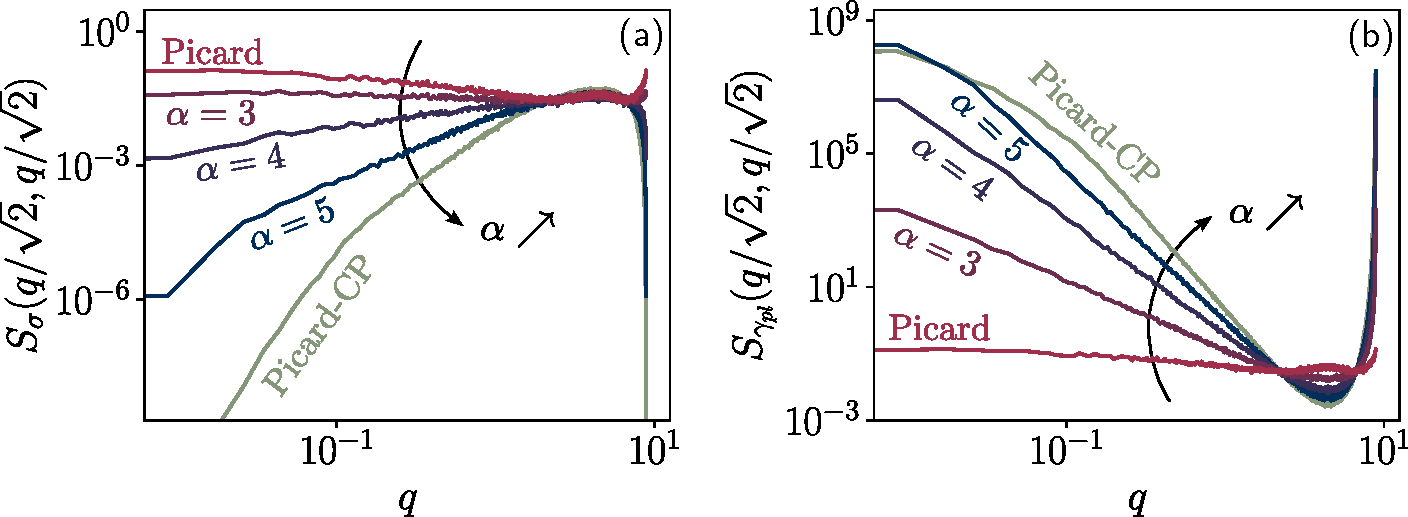
\includegraphics[width=\textwidth]{Chapitre4/Figures/Correlations/Evol_Sfact.pdf}
	\caption{Évolution des spectres $S_\sigma(\mathbf{q})$ (a) et $S_{\epsilon_{pl}}(\mathbf{q})$ (b) pour les généralisations du modèle de Picard le long de la diagonale $(q_x=\frac{q}{\sqrt{2}},q_y=\frac{q}{\sqrt{2}})$.}
	\label{fig:SfactAlphaPicard}
\end{figure}

\begin{table}[h]
\centering
\begin{tabular}{ccc}
\hline \hline $\alpha$ & $\alpha_\text{HU}$ & $\eta$ \\
\hline 
$\text{FES}^\pm$ & 0.5 & 0.75  \\
Picard-CP & 2.5 & 1.75  \\
5 & 1.5 & 1.25  \\
4 & 0.5 & 0.75  \\
3 & 0 & 0  \\
2 (Picard) & 0 & -1 \\
\hline \hline
\end{tabular}
\caption{Exposants d'hyperuniformité déterminés dans les modèles $\alpha$-Picard, Picard-CP et $\text{FES}^\pm$.}
\label{tab:expoHU}
\end{table}

\subparagraph{}Nous remarquons alors une évolution a priori continue de l'hyperuniformité de contrainte, avec un caractère évanescent de $S_\sigma(\mathbf{q})$ perdu autour du point $\alpha=3$. Pour le cas classique du modèle de Picard, il semble donc que la contrainte ne présente pas d'hyperuniformité.

\subparagraph{}Si l'on regarde en parallèle l'évolution de $S_{\epsilon_{pl}}(\mathbf{q})$, nous observons la tendance inverse. L'exposant de rugosité apparent augmente à mesure que la portée de redistribution diminue. Il passe de $\eta\approx -1$ pour le modèle de Picard\footnote{La valeur négative trouvée ici est simplement extraite de l'étude du spectre. Son interprétation physique en tant qu'exposant de rugosité est peut-être discutable.} à $\eta\approx 1.75$ pour le modèle Picard-CP. L'interface perd donc sa rugosité dans le cas classique. Il est par ailleurs intéressant de noter que les modèles Picard-CP et le modèle 5-Picard sont décrits par des exposants différents, et différents du modèle $\text{FES}^\pm$, suggérant bien une différence marquée par la présence des modes zéros pour $\alpha>4$. De plus pour $\alpha=4$, nous obtenons les exposants de la classe CDP, suggérant le début d'une zone similaire entre les modèles type dépiégeage et type transition vers l'écoulement (nommée LP dans la section précédente).

\subparagraph{}Cette évolution conjointe de $\alpha_\text{HU}$ et $\eta$ est bien compatible avec la relation \autoref{eq:scalingHULP}, qui n'est autre qu'une traduction de la règle d'évolution de la contrainte. Plus la répartition de contrainte est hyperuniforme, plus l'interface est rugueuse.

\subparagraph{}Cette analyse structurelle permet donc d'appuyer le paysage présenté à la section précédente, notamment en confortant une différence entre la classe CDP et la classe CDP-0. Qui plus est, elle permet de clarifier la notion d'hyperuniformité dans les modèles élastoplastiques et son lien direct avec la rugosité de l'interface, représentée ici par la répartition spatiale de plasticité accumulée. Si le comportement champ moyen du dépiégeage est retrouvé autour du point $\alpha \approx 3$, celui-ci est encore une fois dépassé pour des plus grandes portées. Nous rappelons que ce point était aussi celui autour duquel la convexité de la transition et le comportement des fluctuations s'inversaient.

\section{Caractérisation dynamique et avalanches}

\subparagraph{}Une dernière façon de caractériser la transition vers l'écoulement est du point de vue dynamique. C'est-à-dire en analysant les avalanches qui la composent. Dans le cas de la transition vers l'écoulement, ces avalanches ont été l'objet d'études exhaustives, aussi bien expérimentalement que numériquement \cite{sun_plasticity_2010, lauridsen_shear-induced_2002, salerno_effect_2013, oyama_unified_2021, talamali_avalanches_2011, liu_driving_2016}.

\subsection{Avalanches de plasticité}

\subparagraph{}Dans les systèmes de particules étudiés lors des chapitres précédents, les avalanches correspondent à des évènements corrélés d'activité proches du point critique, et donc sans échelle. Dans le cas de la transition vers l'écoulement, les avalanches correspondent de manière tout à fait analogue à des évènements d'activité proches du point critique, l'activité étant ici assimilée à la plasticité.

\subsubsection{Phénoménologie}

\paragraph{Dynamique à l'approche du point critique}

\subparagraph{}Reprenons ici le système modèle étudié jusqu'à présent d'un matériau soumis à un cisaillement simple. Dans le cas où le taux de cisaillement $\dot{\gamma}$ est imposé, après une période transitoire, la contrainte $\Sigma$ portée par le matériau fluctue autour de sa valeur moyenne. Pour des forçages relativement grands, cette évolution autour de la valeur moyenne se fait de manière continue (voir \autoref{fig:av_pheno_EPM}-(a1)). Mais à mesure que $\dot{\gamma}$ tend vers 0, la dynamique du système devient intermittente \cite{nicolas_deformation_2018} : la contrainte portée par le système alterne des phases d'augmentation constante et de décroissance brutale. L'évolution de $\Sigma$ au cours du temps prend alors la forme décrite à la \autoref{fig:av_pheno_EPM}-(a2), analogue à des dents de scie. Ces sauts brutaux dans la contrainte globale portée par le système correspondent aux avalanches de plasticité dans le matériau. En effet, à mesure que $\dot{\gamma}\rightarrow 0$, le système s'approche naturellement de son point critique, donnant lieu à des évènements de plasticité de plus en plus corrélés, et sans échelle caractéristique.

\paragraph{Observables d'intérêt}

\subparagraph{}De la même manière que dans le cas des systèmes de particules, on peut caractériser ces évènements dynamiques par leur taille $S$ et leur durée $T$. Dans le cas des avalanches de plasticité, on définit communément la taille $S$ d'une avalanche via la chute de contrainte $\Delta\Sigma$ associée selon :

\begin{equation}
	S = \Delta\Sigma\times L^D
\end{equation}

\noindent avec $L^D$ le volume du système afin de rendre cette quantité extensive. D'autre part, la durée d'une avalanche correspond simplement à la durée sur laquelle a lieu cette chute brutale de contrainte.

\subparagraph{}Ces deux quantités $S$ et $T$ suivent alors des distributions de probabilité en loi de puissance :

\begin{equation}
	P(S) \sim S^{-\tau}f\left( \frac{S}{S_c} \right), \quad P(T) \sim T^{-\tau^\prime}f\left( \frac{T}{T_c} \right)
	\label{eq:AvalancheDistrib}
\end{equation}

\noindent avec $\tau$ et $\tau^\prime$ les exposants d'avalanche, $f$ et $g$ des fonctions à décroissance rapide, et $S_c$ et $T_c$ les cut-offs de taille et de durée du système, de la même manière que dans le cas du dépiégeage présenté au \autoref{chapter:introduction}. Tracées sur une échelle logarithmique, ces distributions prennent alors la forme donnée à la \autoref{fig:av_pheno_EPM}-(b)-(c).

\begin{figure}[h]
	\centering
	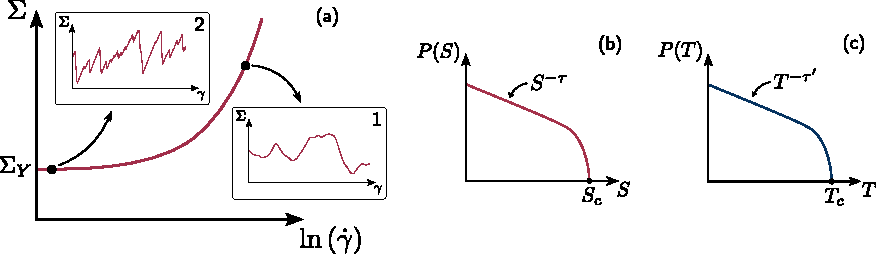
\includegraphics[width=\textwidth]{Chapitre4/Figures/Avalanches/Pheno.pdf}
	\caption{Phénoménologie des avalanches de plasticité dans l'écoulement des fluides à seuil. (a) Évolution de la contrainte avec la déformation globale à différentes distances du point critique. (b)-(c) Formes schématiques des distribution de probabilité de tailles et de durées d'avalanche.}
	\label{fig:av_pheno_EPM}
\end{figure}

\subsubsection{L'approche quasistatique comme cadre de référence}

\subparagraph{}Afin d'observer les avalanches de la manière la mieux définie possible, il faut se placer au plus proche du point critique, i.e. $\dot{\gamma} = 0$. Une méthode alors naturelle est d'utiliser un protocole quasistatique. La méthode quasistatique revient à utiliser un forçage dont l'échelle caractéristique de temps est très grande devant tout autre temps caractéristique (durée des avalanches, temps de réarrangement, ...). Elle permet alors une séparation d'échelle entre le phénomène de forçage (cisaillement) et de relaxation (avalanches). En pratique, partant d'un état initial élastique en tout point, le système est forcé infiniment lentement jusqu'à ce que le premier réarrangement plastique ait lieu. Le forçage est alors suspendu et on laisse le système relaxer par une suite de réarrangements plastiques : ce sont les avalanches. L'avalanche se poursuit alors jusqu'à ce que le système retourne à un état élastique en tout point, et l'on opère un nouveau forçage jusqu'au déclenchement de la prochaine avalanche. L'évolution de la contrainte portée par le système en fonction de sa déformation prend alors la forme définie sur la \autoref{fig:AQS}.

\begin{figure}[h]
	\centering
	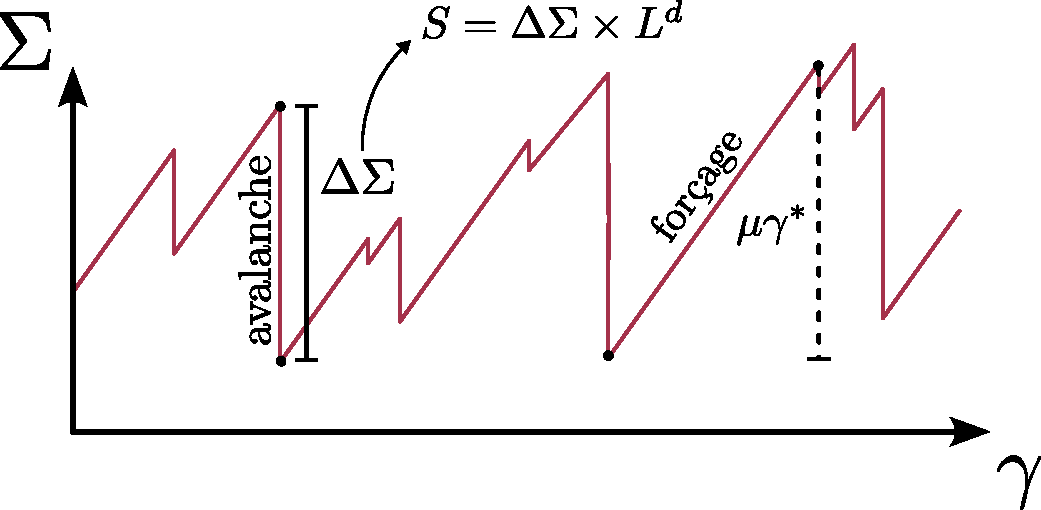
\includegraphics[width= 0.6\textwidth]{Chapitre4/Figures/Avalanches/AQS.pdf}
	\caption{Évolution schématique de la contrainte avec la déformation globale dans un protocole quasistatique.}
	\label{fig:AQS}
\end{figure}

\subparagraph{}Étant dans ce cas à la valeur critique du paramètre $\dot{\gamma} = 0^+$, les cut-offs sur la distribution des tailles et des durées d'avalanche dépendent uniquement de la taille $L$ du système étudié selon :

\begin{equation}
	S_c \sim L^{d_f}, \quad T_c \sim L^z
\end{equation}

\noindent avec $d_f$ la dimension fractale et $z$ l'exposant dynamique. Plus $d_f$ est grand, plus les avalanches sont compactes.

\subparagraph{}En pratique, ce protocole quasistatique n'est pas rigoureusement applicable en laboratoire. Le compromis à faire est alors de trouver un forçage $\dot{\gamma}$ suffisamment faible pour opérer la séparation d'échelle tout en le gardant suffisamment grand pour limiter la durée totale de l'expérience. Dans certaines approches théoriques ou numériques, il est cependant possible de réduire le temps nécessaire aux phases de forçage lent, rendant ainsi ce protocole idéal pour la mesure des avalanches (voir la section suivante).

\subsubsection{Résultats dans les différents cadre d'étude}

\subparagraph{}D'un point de vue analytique, comme nous l'avons mentionné à la \autoref{sec:TheoEPM}, la non-positivité du propagateur de redistribution d'Eshelby rend la résolution théorique du problème difficile. Une approche de théorie des champs ne permet donc pas de décrire les avalanches de plasticité dans le cadre de la transition vers l'écoulement. Toutefois, la phénoménologie de ces avalanches étant parfaitement similaire à celle observée dans le cas du dépiégeage, il est usuel d'utiliser les prédictions associées à ce deuxième phénomène comme base de comparaison.

\subparagraph{}Dans le cas du dépiégeage, les méthodes du groupe de renormalisation sont capables de prédire l'existence d'avalanches et les distributions de probabilité associées \cite{wiese_theory_2022}. Notamment, ces méthodes permettent la prédiction des valeurs des exposants critiques comme $\tau$. Dans la limite de champ moyen, la théorie prédit un exposant pour les tailles d'avalanches $\tau = 3/2$ \cite{le_doussal_size_2009}.

\subparagraph{}Du côté expérimental, les avalanches de plasticité ont été mesurées dans de nombreux systèmes, à de nombreuses échelles et sous différentes conditions. Ces réalisations cherchent alors à rapprocher ou différencier ces avalanches de celles du dépiégeage et notamment des prédictions de champ moyen. Elles ont par exemple été mesurées dans des mousses cisaillées  dans \cite{lauridsen_shear-induced_2002}, donnant un exposant $\tau\approx 0.8$, dans des verres métalliques dans \cite{sun_plasticity_2010} donnant cette fois $\tau\approx 1.4-1.5$ ou encore dans un milieu granulaire  dans \cite{denisov_universality_2016} amenant comme dans le second cas à un comportement compatible avec l'attendu de champ moyen. Dans la plupart des cas, les expériences donnent lieu à des distributions d'avalanches s'étendant sur très peu de décades. Par ailleurs, cette grande variabilité des propriétés statistiques mesurées vient probablement de la précision nécessaire à ces mesures et de la difficulté d'étudier un système parfaitement contrôlé \cite{bonn_yield_2017}. Afin de qualifier l'universalité de ces avalanches il est alors plus simple de passer par une approche numérique.

\subparagraph{}Via les approches de type dynamique moléculaire notamment, il est facilement possible de mettre en oeuvre un protocole de cisaillement quasistatique. Par exemple, dans \cite{makinen_avalanches_2025}, les auteurices ont cisaillé des verres métalliques CuZrAl et CuZr préparés de différentes manières. Sous forçage quasistatique, les tailles d'avalanches suivent une loi de puissance avec $\tau \approx 1.16$. Dans \cite{salerno_effect_2013}, les auteurs ont étudié les avalanches sous cisaillement quasistatique d'un autre verre, et ce pour différents régimes inertiels. En deux ou trois dimensions, l'étude révèle un exposant $\tau \approx 1.2-1.3$ et donc diffère aussi du cadre champ moyen. Néanmoins, dans le travail \cite{oyama_unified_2021}, les auteurices ont souligné l'importance d'une analyse attentive des distributions d'avalanches. En effet, ces dernières pouvant présenter des bosses au niveau de leur cut-off, la mesure de l'exposant $\tau$ peut s'en trouver grandement affectée si celles-ci sont ignorées. Par une analyse attentive, les auteurices ont alors déduit de leurs résultats une compatibilité avec $\tau=3/2$. Le problème est que ces simulations font intervenir de très nombreux degrés de liberté et sont donc très coûteuses numériquement. Elles ne permettent donc pas de simuler des systèmes de grande taille $L$ et d'obtenir des distributions précises sur de larges gammes de tailles $S$. Pour dépasser ces limites, les modèles mésoscopiques comme les modèles élastoplastiques sont donc des outils de choix.

\paragraph{Modèles élastoplastiques}

\subparagraph{}Par les simplifications adoptées, l'étude des avalanches dans les modèles élastoplastiques se révèle très efficace. Ainsi, il est tout à fait envisageable d'étudier ces phénomènes dans des systèmes de grande taille. De plus, il est possible dans ce cas d'implémenter exactement le protocole quasistatique de manière astucieuse. En effet, la distance au seuil microscopique local $\sigma_Y$ étant connue à chaque instant et pour chaque site, il est possible de contourner la phase de forçage infiniment lente par l'ajout direct d'un chargement élastique $\mu\gamma^*$ uniforme sur tous les sites, de telle manière que le site le plus proche de sa contrainte seuil devienne plastique :

\begin{equation}
	\mu\gamma^* = \mathrm{min}(\sigma_{Y,i}-\sigma_i)
\end{equation}

\noindent Il est ainsi possible de passer de la fin d'une avalanche au début de la suivante en un unique pas de temps \cite{lin_scaling_2014}. Cette implémentation, résumée à la \autoref{fig:AQS} et que nous appellerons AQS pour \textit{athermal quasistatic}, permet de produire des statistiques riches pour les observables $S$ et $T$ dans les différents modèles élastoplastiques.

\subparagraph{}En utilisant une dynamique extrêmale proche de l'AQS, Talamali et. al \cite{talamali_avalanches_2011} ont alors mesuré des avalanches distribuées selon $\tau \approx 1.25$, marquant un désaccord avec la théorie champ moyen. Par la suite, Lin et. al \cite{lin_scaling_2014}, Liu et. al \cite{liu_driving_2016} et Ferrero et. al \cite{ferrero_criticality_2019} ont déterminé précisément les distributions de tailles dans le cadre de l'AQS pour mesurer respectivement $\tau \approx 1.2$, $\tau \approx 1.28$ et $\tau\approx 1.33$ en 2D. Ces études s'appuyant toutes sur des modèles différents, un consensus scientifique s'est créé autour d'une valeur universelle $\tau \approx 1.25-1.35$, marquant une différence avec les avalanches de la transition de dépiégeage en champ moyen. Ce consensus se renforce alors par l'extension des mesures à de nouveaux protocoles de déformation \cite{lin_scaling_2014, budrikis_universal_2017}. Dans \cite{budrikis_universal_2017} notamment, les avalanches obtenues sous un grand nombre de déformations différentes donnent toutes $\tau\approx1.28$. 

\subparagraph{}Par ailleurs, avec ce protocole d'AQS et les protocoles apparentés, la dimension fractale $d_f$ associée aux avalanches prend elle aussi une valeur avec de faibles variations, autour de $d_f \approx 1$ \cite{liu_driving_2016, lin_scaling_2014, ferrero_criticality_2019}. Ce résultat est central, puisqu'il met en évidence des avalanches de plasticité peu compactes, presque linéaires, à l'image des cartes de plasticité discutées à la \autoref{fig:MapsOfActSR} et des bandes de cisaillement observées dans les mêmes systèmes \cite{martens_spontaneous_2012}. Ces évènements contrastent alors avec ceux du dépiégeage pour lesquels on mesure une plus grande compacité avec $d_f \geq D$ \cite{wiese_theory_2022, le_priol_spatial_2021}. En effet, on a dans le cas du dépiégeage un lien direct entre dimension fractale et exposant de rugosité : $d_f = D + \eta$, avec $\eta = 0$ la valeur limite minimale en champ moyen\footnote{Dans le cas des avalanches mesurées avec le protocole AQS, cette relation semble toujours vérifiée si l'on se base sur les mesures de l'exposant de rugosité dans le modèle de Picard (voir \autoref{sec:HUEPM})}.

\subparagraph{}Ces résultats semblent assez robustes et placent les avalanches comme un descripteur possible de criticalité et d'universalité. Toutefois, comme nous l'avons relevé précédemment, la qualification d'un comportement critique peut se jouer sur une détermination très précise des exposants. Afin que notre étude soit conclusive il faut donc prêter une grande attention à nos méthodes et leurs implications, notamment si l'on s'éloigne des protocoles de référence.

\subsection{Avalanches à contrainte imposée}

\subparagraph{}L'analyse que nous faisons de la transition vers l'écoulement se place dans le cadre des transitions de phase absorbantes. Le paramètre de contrôle naturel à fixer est donc la contrainte globale $\Sigma$. Afin de préserver notre cadre et de décrire les évènements proches du point critique sous la même dynamique, nous choisissons d'étudier les avalanches dans le système à contrainte imposée. Cela contraste avec la plupart des résultats précédemment exposés puisque l'approche quasistatique se fait naturellement à taux de cisaillement imposé ($\dot{\gamma}\rightarrow 0$).

\subparagraph{}Cette approche que nous proposons, en plus d'avoir une motivation conceptuelle majeure dans notre cas, peut trouver un intérêt pour la modélisation des systèmes réels. En effet, dans certains cas de dynamique d'avalanche de plasticité, le paramètre imposé adapté est la contrainte plutôt que le taux de cisaillement, et parfois même un possible mélange des deux.

\subsubsection{Un problème d'états absorbants}

\paragraph{Dynamique proche du point critique en taille finie}

\subparagraph{}Pour étudier les avalanches qui composent la dynamique, il est nécessaire de se placer au plus proche du point critique $\Sigma = \Sigma_c$. Comme nous l'avons vu précédemment, lorsque que nous imposons au système une contrainte $\Sigma < \Sigma_c$, il finit par tomber dans un état absorbant où le matériau est élastique en tout point (i.e. tous les sites sont dans l'état $n_i = 0$). Nous appellerons un tel état un état élastique. La dynamique étant in fine piégée dans cet état élastique, il est impossible de sonder statistiquement les évènements constituant l'état stationnaire en-dessous du point critique, et donc les avalanches. Pour un système de taille fini, ce problème s'étend même aux cas $\Sigma \gtrsim \Sigma_c$. En effet, par ses fluctuations, le système peut atteindre un état élastique au cours de la dynamique et donc y rester piégé éternellement (voir l'exemple de simulation sur la \autoref{fig:PbContrainte}-(a)).

\begin{figure}[h]
	\centering
	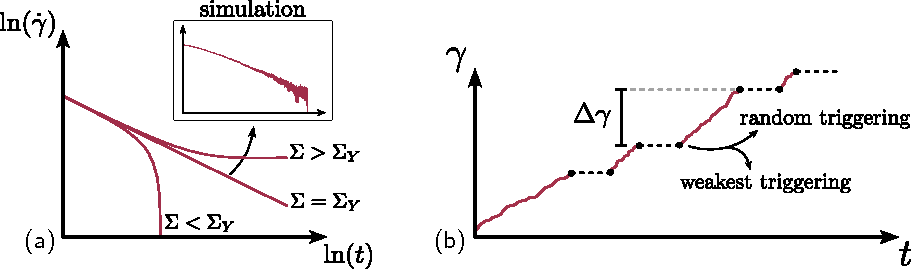
\includegraphics[width=\textwidth]{Chapitre4/Figures/Avalanches/PbContrainte.pdf}
	\caption{Problème posé par l'étude des avalanches à contrainte imposée (a) et résolution par la mise en place de protocolesde réactivation (b).}
	\label{fig:PbContrainte}
\end{figure}

\paragraph{Redéfinition des avalanches}

\subparagraph{}Afin de pouvoir étudier les évènements proches de la transition à contrainte imposée, il est donc nécessaire de réactiver le système à chaque fois qu'il tombe dans un état élastique. Nous définissons alors les avalanches de plasticité comme les évènements d'activité ayant lieu entre deux réactivations du système. Cette redéfinition reste proche de celle présentée précédemment puisque dans le cas quasistatique, une avalanche correspond aussi à un évènement entre deux états élastiques, seulement générés différemment.

\subparagraph{}Il faut cependant réadapter la définition de certaines observables associées comme la taille $S$ de ces avalanches. En effet, dans ce cas, la contrainte ne varie pas au cours de l'avalanche et la définition $S=\Delta\Sigma \times L^D$ devient obsolète. Cependant, lors de ces avalanches, la déformation globale du système $\gamma$ augmente de manière analogue. En notant $\Delta\gamma$ la différence de déformation entre le début et la fin d'une avalanche, nous proposons de caractériser la taille d'une avalanche par $S=\Delta\gamma \times L^D$. Pour éviter toute confusion dans la suite de cette étude, nous noterons $S_\Sigma$ la taille des avalanches à taux de cisaillement imposé et $S_\gamma$ celle des avalanches à contrainte imposée.

\subparagraph{}Un problème majeur cependant est qu'au contraire du cas quasistatique, la réactivation des états élastiques en contrainte imposée n'a pas de forme naturelle. Dans le cas quasistatique, l'état élastique généré après une avalanche est réactivé en effectuant un forçage uniforme sur le système qui augmente sa contrainte globale (quantité $\mu\gamma^*$ sur la \autoref{fig:AQS}). La contrainte devant être conservée pendant la simulation, cette méthode ne peut pas être appliquée ici.

\subparagraph{}Il existe alors plusieurs méthodes possibles pour réactiver le système tout en conservant sa contrainte globale. La question est donc de savoir si toutes ces méthodes sont équivalentes et laquelle semble la plus adaptée pour mener notre étude dynamique de la transition. Si des protocoles d'avalanches à contrainte imposée ont déjà été mis en oeuvre, notamment dans les travaux cités précédemment \cite{budrikis_universal_2017, lin_scaling_2014}, l'influence spécifique du protocole a été mise de côté. Cela laisse à penser que tous seraient équivalents, qu'ils soient à contrainte ou déformation imposée. Notre question pratique se révèle donc d'une seconde utilité : éclairer cette zone d'ombre de la litérature.

\subsubsection{Importance du choix d'un protocole}

\label{sec:imp_prot}

\subparagraph{}Dans cette sous-section, nous reprenons les résultats publiés dans \cite{jocteur_protocol_2025}. La publication complète est présentée dans la \autoref{sec:article2} mais ne sera pas complètement discutée ici afin de ne se concentrer que sur les informations essentielles pour notre propos.

\paragraph{Protocoles étudiés}

\subparagraph{}Afin de déterminer l'importance du protocole de réactivation dans l'analyse des avalanches à contrainte imposée, nous en étudions deux : le \textit{random triggering protocol}\footnote{traduit en français par \textit{protocole par déclenchement aléatoire}} (RTP) et le \textit{weakest triggering protocol}\footnote{traduit en français par \textit{protocole par déclenchement du plus faible}} (WTP).

\subparagraph{}Dans le cadre du RTP, le système est soumis à sa contrainte critique $\Sigma = \Sigma_c$ déterminée dans la \autoref{sec:CP_Picard}. \`A chaque fois que le système tombe dans un état élastique, nous le réactivons en rendant plastique un site au hasard. Ceci se fait alors en agissant directement sur la variable $n_i$ et donc sans modification du champ de contrainte $\{\sigma_i\}$. Nous notons que ce protocole ressemble fortement à un protocole déjà mentionné dans la litérature \cite{lin_scaling_2014}.

\subparagraph{}Le WTP ressemble alors fortement à ce premier protocole. Simplement, cette fois ce n'est pas un site aléatoire qui est rendu plastique mais nous choisissons spécifiquement le site le plus proche de sa contrainte seuil, i.e. avec la valeur minimale de $\sigma_Y - \sigma_i$. En ce sens, cette réactivation ressemble au protocole AQS. En effet, après un forçage uniforme du système c'est le site le plus proche de son seuil qui devient plastique en premier. De la même façon, un protocole analogue à celui-ci a déjà été décrit dans un précédent travail \cite{lin_scaling_2014}.

\subparagraph{}Enfin, afin d'avoir un point de comparaison, nous étudions en parallèle le protocole classique de l'AQS. Pour caractériser précisément les avalanches pour chacun de ces protocoles, nous les simulons pour générer dans l'état stationnaire\footnote{L'état stationnaire est considéré atteint lorsque les propriétés statistiques des avalanches sont elles aussi stationnaires.} environ $5\times 10^5$ avalanches dans un système de taille $L=512$.

\paragraph{Comparaisons statistiques}

\subparagraph{}Les distributions de tailles d'avalanche obtenues pour ces trois protocoles sont présentées à la \autoref{fig:DistribProtocols}. Comme on peut le remarquer, les distributions prennent des formes très différentes selon le protocole. Si les résultats pour l'AQS sont retrouvés avec $\tau\approx 1.35$, dans le cadre du RTP l'exposant estimé semble être légèrement plus grand avec $\tau \approx 1.5$. Il montre aussi une forme de cut-off différente, faisant apparaître une bosse aux grandes tailles. Par ailleurs, le WTP présente des avalanches largement distribuées mais pas selon une loi de puissance claire, rendant de ce fait impossible l'estimation de $\tau$. Nous remarquons par ailleurs que les cut-offs dans le cas des protocoles à contrainte imposée sont bien plus grands que celui dans le cas de l'AQS. Cette première analyse montre donc clairement que les protocoles de génération d'avalanches influent fortement sur les évènements générés. Il est donc très important de comparer des approches équivalentes pour conclure sur une comparaison des avalanches dans différents systèmes.

\begin{figure}[h]
	\centering
	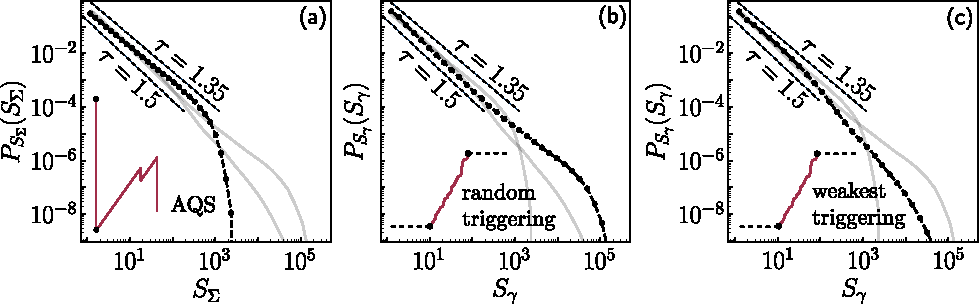
\includegraphics[width=\textwidth]{Chapitre4/Figures/Avalanches/Comparaison_Distrib.pdf}
	\caption{Distributions des tailles d'avalanche pour les trois différents protocoles étudiés : (a) AQS, (b) RTP, (c) WTP. Les avalanches sont générées dans un système de taille $L=512$.}
	\label{fig:DistribProtocols}
\end{figure}

\subparagraph{}Pour comparer plus précisément ces protocoles, nous menons une analyse de taille finie sur les distributions de tailles et de durées d'avalanche qu'ils produisent. D'après les lois d'échelles présentées à l'\autoref{eq:AvalancheDistrib}, en mesurant ces distributions pour différentes tailles de système et en opérant le redimensionnement suivant :

\begin{equation}
	S \rightarrow \frac{S}{L^{d_f}}, \quad P(S) \rightarrow \frac{P(S)}{L^{-d_f\tau}},\quad S \rightarrow \frac{T}{L^{z}}, \quad P(T) \rightarrow \frac{P(T)}{L^{-z\tau^\prime}}
\end{equation}

\noindent les distributions pour différentes tailles se superposent sur une même courbe maîtresse. Ainsi, cela constitue une méthode graphique précise et efficace pour la détermination des exposants $(\tau, \tau^\prime, d_f, z)$. En suivant cette méthode pour les protocoles AQS et RTP, nous obtenons les résultats présentés à la \autoref{fig:CollapseAv}.

\begin{figure}[h]
	\centering
	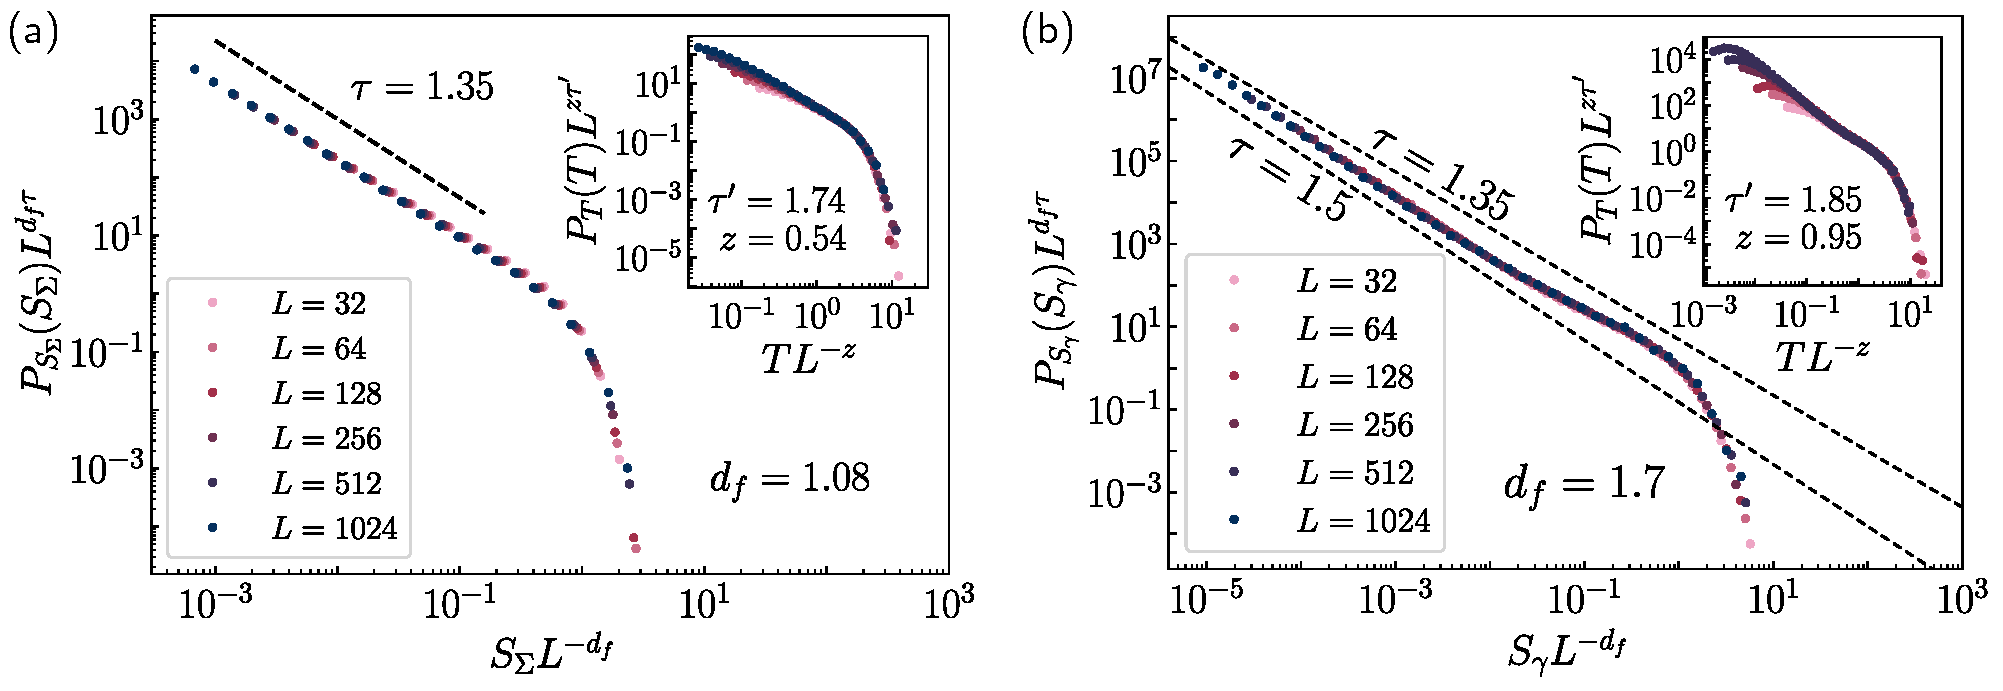
\includegraphics[width=\textwidth]{Chapitre4/Figures/Avalanches/Collapse.pdf}
	\caption{Analyse d'échelle de taille finie des distributions de tailles (figures principales) et de durées (encarts) d'avalanches pour les protocoles AQS (a) et RTP (b).}
	\label{fig:CollapseAv}
\end{figure}

\subparagraph{}La première chose à noter est que la superposition des courbes est remarquable dans les deux cas. La différence d'exposant d'avalanche $\tau$ est par ailleurs bien confirmée entre ces deux protocoles avec $\tau = 1.35$ pour l'AQS et $\tau=1.5$ pour le RTP. D'autre part, nous retrouvons approximativement pour l'AQS les valeurs attendues pour la dimension fractale $d_f\approx 1.1$ et l'exposant dynamique $z\approx 0.55$ \cite{liu_driving_2016, lin_scaling_2014}. Pour le RTP cependant, ces exposants de structure sont très différents avec $d_f \approx 1.7$ et $z\approx 0.95$. Ces mesures identifient alors des évènements plus longs et surtout plus compacts dans le cas du RTP, bien que l'on ait toujours $d_f < D$. D'autre part, dans le cas du WTP, un tel redimensionnement n'est pas réalisable de manière satisfaisante \cite{jocteur_protocol_2025}.

\subparagraph{}Cette caractérisation plus précise confirme alors une différence de nature fondamentale entre les évènements générés par différents protocoles.

\subsubsection{Le protocole RTP comme protocole naturel}

\subparagraph{}S'il donne lieu à des résultats très différents de l'AQS, le protocole RTP semble tout de même être un protocole à contrainte imposé cohérent et solide. Il est par ailleurs possible de rationaliser les différences mesurées entre ces deux protocoles \cite{jocteur_protocol_2025}. Nous montrons enfin à la \autoref{sec:article2} qu'il répond aux mêmes lois d'échelle que le protocole classique de l'AQS. Ces éléments font donc du RTP un candidat de choix pour l'analyse dynamique de la transition vers l'écoulement à contrainte imposée, de la même façon que l'AQS l'est dans le cas du taux de cisaillement imposé. 

\subparagraph{}Ce choix maintenant évident est en fait plus naturel qu'il n'y paraît. En effet, dans la \autoref{sec:methodeFSS}, nous avions déjà défini le champ d'activation $h$ comme un équivalent du forçage élastique à contrainte imposée. Or de la même manière que l'AQS correspond à la limite $\dot{\gamma} \rightarrow 0$, le RTP correspond à la limite $h\rightarrow 0$. Ainsi, même si son interprétation physique est moins directe, le protocole RTP correspond bien en quelque sorte à une limite critique du processus d'avalanches en contrainte imposée. C'est donc ce protocole que nous allons utiliser pour caractériser les avalanches dans les généralisations du modèle de Picard présentées précédemment.

\subsection{Influence de la portée sur les avalanches en contrainte imposée}

\subparagraph{}De la même manière que la portée d'interaction modifie les exposants critiques (\autoref{sec:criticalitealphapicard}) et les propriétés d'hyperuniformité (\autoref{sec:HUEPM}), nous proposons d'évaluer son influence sur les propriétés d'avalanches. Notamment, nous déterminons comment évoluent les différents exposants caractérisant ces phénomènes avec la portée $\alpha$, afin de voir si les propriétés dynamiques suivent une évolution similaire à celle des autres propriétés critiques.

\subsubsection{Avalanches dans le modèle $\alpha$-Picard}

\label{sec:Av_PicardMain}

\paragraph{Méthode}

\subparagraph{}Afin d'étudier les avalanches à contrainte imposée dans le modèle $\alpha$-Picard, nous générons des avalanches en suivant le protocole RTP pour différentes tailles de système et ce pour $\alpha = \{2, 3, 4, 5\}$. Nous déterminons alors les différents exposants caractéristiques par une analyse d'échelle en taille finie comme dans le cas du modèle de Picard (voir \autoref{sec:imp_prot}). 

\subparagraph{}En plus de la taille et de la durée des avalanches, nous caractérisons leur étendue spatiale $A$. Celle-ci correspond en fait à la surface, exprimée en nombre de sites, sur laquelle a pris part l'avalanche. De la même manière que pour les deux autres observables, nous postulons que cette quantité est distribuée selon :

\begin{equation}
	P(A) \sim A^{-\tau^{\prime\prime}}h\left( \frac{A}{A_c} \right),\quad A_c \sim L^\chi
	\label{eq:distA}
\end{equation}

\noindent avec $h$ une fonction à décroissance rapide et $A_c$ le cut-off associé. Ce cette façon, $\chi=D=2$ signifie que les avalanches occupent au maximum toute la surface du système. Cette quantité permet alors d'offrir une nouvelle caractérisation des avalanches, utile à l'interprétation des résultats qui suit.

\paragraph{\'Evolution des exposants}

\subparagraph{}Les redimensionnements effectués pour obtenir la meilleure estimation des exposants sont présentés à la \autoref{fig:Av_rescale_alpha3} dans le cas du modèle 3-Picard. Ces mêmes figures sont reportées en annexe pour les autres modèles et nous reportons les exposants déterminés dans le \autoref{tab:expocritav}. Globalement la superposition des courbes est très convaincante dans chacun des cas et pour toutes les distributions. Cela valide alors notre approche à tout $\alpha$, notamment l'ansatz de l'\autoref{eq:distA}. Notons par ailleurs que ces résultats sont des résultats préliminaires non publiés qui nécessitent encore quelques améliorations. Néanmoins, leur état actuel permet d'effectuer certaines observations.

\begin{figure}[h]
	\centering
	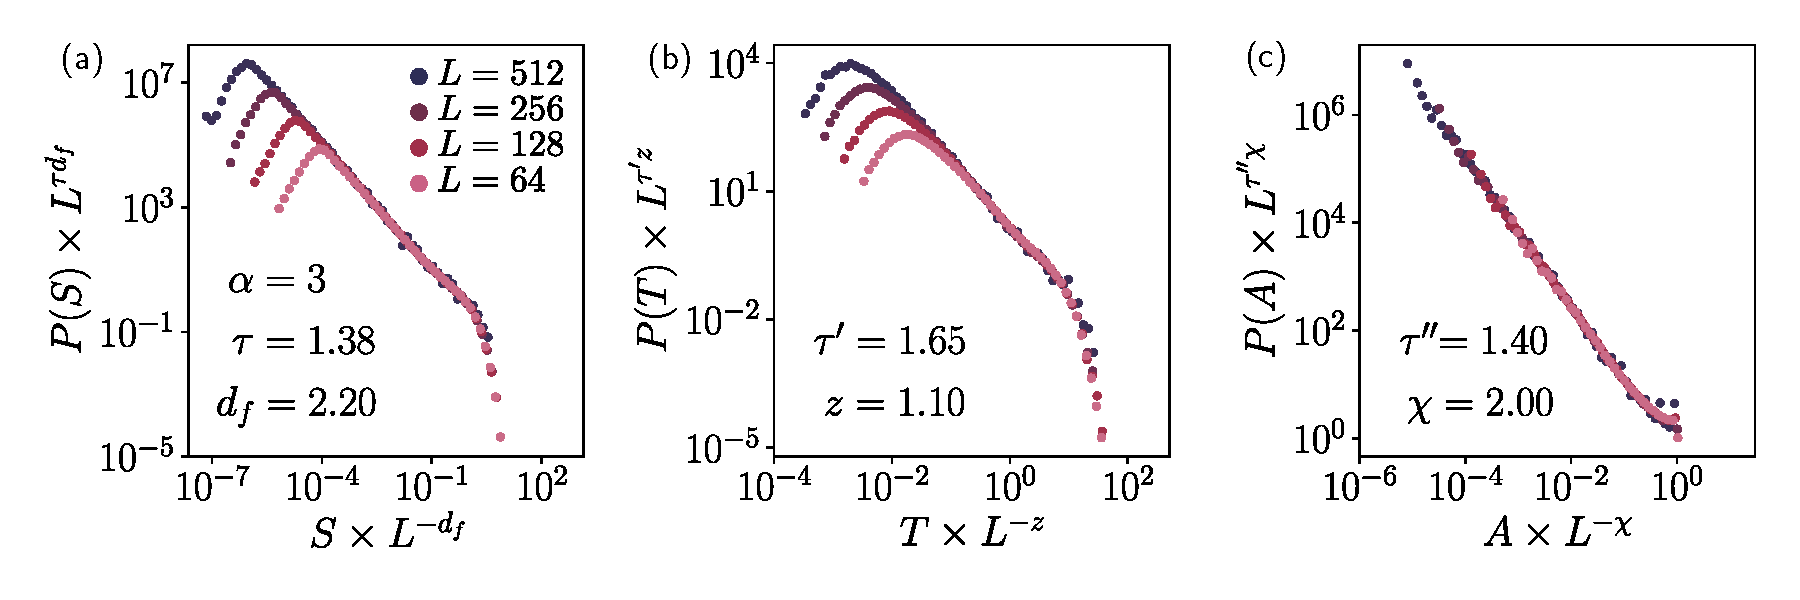
\includegraphics[width=\textwidth]{Chapitre4/Figures/Avalanches/Rescale_Av_alpha3.pdf}
	\caption{Distributions de tailles (a), de durées (b) et de surfaces (c) d'avalanche redimensionnées dans le modèle 3-Picard. Les exposants permettant cette superposition sont reportés dans le \autoref{tab:expocritav}}
	\label{fig:Av_rescale_alpha3}
\end{figure}

\begin{table}[h]
\centering
\begin{tabular}{ccccccc}
\hline \hline $\alpha$ & $\tau$ & \multicolumn{1}{c}{$\tau^\prime$} & $\tau^{\prime\prime}$ & $d_f$ & $z$ & $\chi$ \\
\hline 5 & 1.3 & 1.5 & 1.35 & 2.8 & 1.55 & 2 \\
4 & 1.3 & 1.47 & 1.37 & 2.8 & 1.55 & 2 \\
3 & 1.38 & 1.65 & 1.4 & 2.2 & 1.1 & 2 \\
2 (Picard) & 1.50 & 1.85 & 1.48 & 1.7 & 0.95 & 1.75 \\
\hline \hline
\end{tabular}
\caption{Exposants d'avalanches déterminés dans les modèles $\alpha$-Picard}
\label{tab:expocritav}
\end{table}

\subparagraph{}Nous remarquons d'abord que les exposants $\tau$, $\tau^\prime$ et $\tau^{\prime\prime}$ caractérisant les lois de puissance ont tous tendance à augmenter à mesure que la portée de l'interaction augmente. Par exemple, on passe de $\tau\approx 1.3$ pour le modèle 5-Picard à $\tau \approx 1.5$ pour le modèle de Picard. Même si ces tendances sont légères, cela signifie que les avalanches sont de moins en moins largement distribuées à mesure qu'$\alpha$ diminue.

\subparagraph{}Par ailleurs, tous les exposants semblent être sensiblement les mêmes pour $\alpha=4$ et $\alpha=5$. Cette observation suggère alors que la région LP-0 identifiée précédemment ne correspond qu'à une variation des exposants critiques statiques, laissant les exposants d'avalanche inchangés sur toute la région. Nous remarquons de plus que cette criticalité est exactement la même que celle de la classe CDP d'après les résultats de la \autoref{sec:AvSusp}, avec $d_f\approx 2.8$ et $z\approx 1.5$. \`A des portées relativement courtes, les modes zéros ne semblent donc pas influencer significativement les avalanches générées via ce protocole.

\subparagraph{}Enfin le point le plus intéressant vient de l'évolution de la dimension fractale avec $\alpha$, qui passe de $d_f\approx 2.8$ pour $\alpha=5$ à $d_f\approx 1.7$ pour le modèle de Picard. Nous rappelons par ailleurs que, comme dans le cas des suspensions discuté au \autoref{chapter:Susp}, cet exposant est à comparer à $D+1$ pour juger de la compacité des avalanches. On passe donc d'avalanches très compactes à courte portée à des avalanches peu compactes à longue portée dans le modèle de Picard. Une manière plus significative de mettre en évidence ce changement est de regarder la projection de l'avalanche sur l'espace de dimension $D$. Dans ce cas là, la quantité d'intérêt est $A$, dont le cut-off est caractérisé par l'exposant $\chi$. Celui-ci passe alors subitement d'une valeur $\chi=D=2$ à $\chi<2$ lorsque l'on passe de $\alpha=3$ à $\alpha=2$. De plus, pour $\alpha=2$ nous mesurons $d_f\approx\chi$. En d'autres termes, autour de $\alpha=3$ la compacité des avalanches change de telle manière qu'elles n'occupent plus, au maximum, la totalité du système. Les avalanches deviennent alors spatialement fractales. Parallèlement, l'exposant dynamique opère un changement significatif autour de $\alpha=3$ où l'on passe de $z>1$ à $z<1$.

\subparagraph{}Comme dans le cas des propriétés critiques statiques et d'hyperuniformité, les avalanches de plasticité ressemblent donc à celles du dépiégeage jusqu'au point $\alpha = 3$, qui marque la limite champ moyen de ce dernier. Toutefois, dans le cas de la transition vers l'écoulement, ce point n'est pas une limite puisqu'il est dépassé par l'évolution des exposant pour $\alpha<3$. Dans cette zone, la structure des avalanches est alors drastiquement différente avec $d_f<D$ et $z<1$, propriétés déjà établies par les études précédentes. Cette étude permet alors de faire émerger ces propriétés d'une évolution globale du modèle avec la portée d'interaction $\alpha$.

\subsubsection{Aparté sur les avalanches écrantées}

\subparagraph{}Si le modèle $\alpha$-Picard est essentiel pour comprendre les propriétés critiques du cas classique, il ne porte pas vraiment de réalité physique. Dans le \autoref{chapter:introduction}, nous avons évoqué une interaction similaire à l'interaction d'Eshelby mais qui, sous écrantage, voit sa portée modifiée. Notamment, elle décroît dans sa partie écrantée comme $1/r^4$, cas étudié ici à contrainte imposée. Un modèle étudiant précisément cette interaction écrantée a été implémenté et ses avalanches sous cisaillement quasistatiques ont été caractérisées. L'étude reléguée à la \autoref{sec:screenedav} montre alors que le système perd sa criticalité dans la zone écrantée. Ceci vient du fait d'une relaxation globale de la contrainte portée uniquement par le site plastique, alors que celle-ci est portée uniformément par tout le système dans le cas du modèle de Picard à taux de cisaillement imposé.

\subparagraph{}Ainsi, au-delà de la longueur d'écrantage, les avalanches de plasticité disparaissent et ne prennent donc pas la forme de celles du modèle 4-Picard. Cette observation, bien qu'annexe, montre alors que la portée d'interaction n'est pas la seule variable pouvant agir sur les propriétés statistiques des avalanches. Dans des situations physiques réelles, tous les aspects de la dynamique doivent donc être soumis à la plus grande attention pour expliquer ces phénomènes.

\section{Conclusion}

\subparagraph{}En conclusion, par l'implémentation d'un modèle élastoplastique, nous avons caractérisé la transition vers l'écoulement des fluides à seuil athermiques. La première phase de caractérisation nous a permis de déterminer les exposants critiques associés à cette transition. Celle-ci a alors permis de mettre en évidence son caractère convexe ($\beta >1$) et le caractère exotique des fluctuations critiques qui se dissipent à l'approche de la transition ($\gamma^\prime<0$). 

\subparagraph{}Par l'étude de variations sur ce modèle, nous avons étudié l'évolution de cette criticalité en fonction de la portée $\alpha$ des interactions associées. Cela nous a permis de mettre en évidence la présence d'une symétrie particulière dans le propagateur de redistribution appelée modes zéros qui modifie le comportement critique du système, et ce même à courte portée. La longue portée inscrite dans ce même propagateur place la transition vers l'écoulement ($\alpha = 2$) dans une zone non-triviale dont la forme a été esquissée. Celle-ci semble séparer une classe de courte portée distincte de la percolation dirigée conservée, appelée CDP-0, d'une zone de champ moyen représentée par le modèle de Hébraud-Lequeux. Si ce comportement est plutôt classique, sa spécificité réside dans le fait que la zone de longue portée s'étend sur une gamme de portées $\alpha$ différente du cas du dépiégeage. Pour $\alpha < 3$, le comportement critique est, comme attendu, très différent de cleui de la transition de dépiégeage, du fait de la possibilité d'interpréter les interactions comme un bruit interne dans cette zone. En revanche, pour $\alpha > 3$, l'évolution des exposants ressemble fortement à celle prédite par le cadre LR-CDP.

\subparagraph{}Cette observation générale se retrouve aussi dans l'évolution des autres propriétés critiques du système. L'hyperuniformité de la répartition de contrainte est perdue conjointement à la rugosité de l'interface pour $\alpha\lesssim 3$ alors qu'elles présentent des caractéristiques similaires au dépiégeage pour $\alpha\gtrsim 3$. D'autre part, les propriétés des avalanches suivent la même tendance. Si des avalanches compactes sont observées pour $\alpha\gtrsim 3$, pour $\alpha\lesssim 3$ les évènements observés sont marqués par une faible compacité avec $d_f < D$, caractéristique de la transition vers l'écoulement. 
